
\documentclass{article} % For LaTeX2e
\usepackage{iclr2026_conference,times}

% Optional math commands from https://github.com/goodfeli/dlbook_notation.
%%%%% NEW MATH DEFINITIONS %%%%%

\usepackage{amsmath,amsfonts,bm}

% Mark sections of captions for referring to divisions of figures
\newcommand{\figleft}{{\em (Left)}}
\newcommand{\figcenter}{{\em (Center)}}
\newcommand{\figright}{{\em (Right)}}
\newcommand{\figtop}{{\em (Top)}}
\newcommand{\figbottom}{{\em (Bottom)}}
\newcommand{\captiona}{{\em (a)}}
\newcommand{\captionb}{{\em (b)}}
\newcommand{\captionc}{{\em (c)}}
\newcommand{\captiond}{{\em (d)}}

% Highlight a newly defined term
\newcommand{\newterm}[1]{{\bf #1}}


% Figure reference, lower-case.
\def\figref#1{figure~\ref{#1}}
% Figure reference, capital. For start of sentence
\def\Figref#1{Figure~\ref{#1}}
\def\twofigref#1#2{figures \ref{#1} and \ref{#2}}
\def\quadfigref#1#2#3#4{figures \ref{#1}, \ref{#2}, \ref{#3} and \ref{#4}}
% Section reference, lower-case.
\def\secref#1{section~\ref{#1}}
% Section reference, capital.
\def\Secref#1{Section~\ref{#1}}
% Reference to two sections.
\def\twosecrefs#1#2{sections \ref{#1} and \ref{#2}}
% Reference to three sections.
\def\secrefs#1#2#3{sections \ref{#1}, \ref{#2} and \ref{#3}}
% Reference to an equation, lower-case.
\def\eqref#1{equation~\ref{#1}}
% Reference to an equation, upper case
\def\Eqref#1{Equation~\ref{#1}}
% A raw reference to an equation---avoid using if possible
\def\plaineqref#1{\ref{#1}}
% Reference to a chapter, lower-case.
\def\chapref#1{chapter~\ref{#1}}
% Reference to an equation, upper case.
\def\Chapref#1{Chapter~\ref{#1}}
% Reference to a range of chapters
\def\rangechapref#1#2{chapters\ref{#1}--\ref{#2}}
% Reference to an algorithm, lower-case.
\def\algref#1{algorithm~\ref{#1}}
% Reference to an algorithm, upper case.
\def\Algref#1{Algorithm~\ref{#1}}
\def\twoalgref#1#2{algorithms \ref{#1} and \ref{#2}}
\def\Twoalgref#1#2{Algorithms \ref{#1} and \ref{#2}}
% Reference to a part, lower case
\def\partref#1{part~\ref{#1}}
% Reference to a part, upper case
\def\Partref#1{Part~\ref{#1}}
\def\twopartref#1#2{parts \ref{#1} and \ref{#2}}

\def\ceil#1{\lceil #1 \rceil}
\def\floor#1{\lfloor #1 \rfloor}
\def\1{\bm{1}}
\newcommand{\train}{\mathcal{D}}
\newcommand{\valid}{\mathcal{D_{\mathrm{valid}}}}
\newcommand{\test}{\mathcal{D_{\mathrm{test}}}}

\def\eps{{\epsilon}}


% Random variables
\def\reta{{\textnormal{$\eta$}}}
\def\ra{{\textnormal{a}}}
\def\rb{{\textnormal{b}}}
\def\rc{{\textnormal{c}}}
\def\rd{{\textnormal{d}}}
\def\re{{\textnormal{e}}}
\def\rf{{\textnormal{f}}}
\def\rg{{\textnormal{g}}}
\def\rh{{\textnormal{h}}}
\def\ri{{\textnormal{i}}}
\def\rj{{\textnormal{j}}}
\def\rk{{\textnormal{k}}}
\def\rl{{\textnormal{l}}}
% rm is already a command, just don't name any random variables m
\def\rn{{\textnormal{n}}}
\def\ro{{\textnormal{o}}}
\def\rp{{\textnormal{p}}}
\def\rq{{\textnormal{q}}}
\def\rr{{\textnormal{r}}}
\def\rs{{\textnormal{s}}}
\def\rt{{\textnormal{t}}}
\def\ru{{\textnormal{u}}}
\def\rv{{\textnormal{v}}}
\def\rw{{\textnormal{w}}}
\def\rx{{\textnormal{x}}}
\def\ry{{\textnormal{y}}}
\def\rz{{\textnormal{z}}}

% Random vectors
\def\rvepsilon{{\mathbf{\epsilon}}}
\def\rvtheta{{\mathbf{\theta}}}
\def\rva{{\mathbf{a}}}
\def\rvb{{\mathbf{b}}}
\def\rvc{{\mathbf{c}}}
\def\rvd{{\mathbf{d}}}
\def\rve{{\mathbf{e}}}
\def\rvf{{\mathbf{f}}}
\def\rvg{{\mathbf{g}}}
\def\rvh{{\mathbf{h}}}
\def\rvu{{\mathbf{i}}}
\def\rvj{{\mathbf{j}}}
\def\rvk{{\mathbf{k}}}
\def\rvl{{\mathbf{l}}}
\def\rvm{{\mathbf{m}}}
\def\rvn{{\mathbf{n}}}
\def\rvo{{\mathbf{o}}}
\def\rvp{{\mathbf{p}}}
\def\rvq{{\mathbf{q}}}
\def\rvr{{\mathbf{r}}}
\def\rvs{{\mathbf{s}}}
\def\rvt{{\mathbf{t}}}
\def\rvu{{\mathbf{u}}}
\def\rvv{{\mathbf{v}}}
\def\rvw{{\mathbf{w}}}
\def\rvx{{\mathbf{x}}}
\def\rvy{{\mathbf{y}}}
\def\rvz{{\mathbf{z}}}

% Elements of random vectors
\def\erva{{\textnormal{a}}}
\def\ervb{{\textnormal{b}}}
\def\ervc{{\textnormal{c}}}
\def\ervd{{\textnormal{d}}}
\def\erve{{\textnormal{e}}}
\def\ervf{{\textnormal{f}}}
\def\ervg{{\textnormal{g}}}
\def\ervh{{\textnormal{h}}}
\def\ervi{{\textnormal{i}}}
\def\ervj{{\textnormal{j}}}
\def\ervk{{\textnormal{k}}}
\def\ervl{{\textnormal{l}}}
\def\ervm{{\textnormal{m}}}
\def\ervn{{\textnormal{n}}}
\def\ervo{{\textnormal{o}}}
\def\ervp{{\textnormal{p}}}
\def\ervq{{\textnormal{q}}}
\def\ervr{{\textnormal{r}}}
\def\ervs{{\textnormal{s}}}
\def\ervt{{\textnormal{t}}}
\def\ervu{{\textnormal{u}}}
\def\ervv{{\textnormal{v}}}
\def\ervw{{\textnormal{w}}}
\def\ervx{{\textnormal{x}}}
\def\ervy{{\textnormal{y}}}
\def\ervz{{\textnormal{z}}}

% Random matrices
\def\rmA{{\mathbf{A}}}
\def\rmB{{\mathbf{B}}}
\def\rmC{{\mathbf{C}}}
\def\rmD{{\mathbf{D}}}
\def\rmE{{\mathbf{E}}}
\def\rmF{{\mathbf{F}}}
\def\rmG{{\mathbf{G}}}
\def\rmH{{\mathbf{H}}}
\def\rmI{{\mathbf{I}}}
\def\rmJ{{\mathbf{J}}}
\def\rmK{{\mathbf{K}}}
\def\rmL{{\mathbf{L}}}
\def\rmM{{\mathbf{M}}}
\def\rmN{{\mathbf{N}}}
\def\rmO{{\mathbf{O}}}
\def\rmP{{\mathbf{P}}}
\def\rmQ{{\mathbf{Q}}}
\def\rmR{{\mathbf{R}}}
\def\rmS{{\mathbf{S}}}
\def\rmT{{\mathbf{T}}}
\def\rmU{{\mathbf{U}}}
\def\rmV{{\mathbf{V}}}
\def\rmW{{\mathbf{W}}}
\def\rmX{{\mathbf{X}}}
\def\rmY{{\mathbf{Y}}}
\def\rmZ{{\mathbf{Z}}}

% Elements of random matrices
\def\ermA{{\textnormal{A}}}
\def\ermB{{\textnormal{B}}}
\def\ermC{{\textnormal{C}}}
\def\ermD{{\textnormal{D}}}
\def\ermE{{\textnormal{E}}}
\def\ermF{{\textnormal{F}}}
\def\ermG{{\textnormal{G}}}
\def\ermH{{\textnormal{H}}}
\def\ermI{{\textnormal{I}}}
\def\ermJ{{\textnormal{J}}}
\def\ermK{{\textnormal{K}}}
\def\ermL{{\textnormal{L}}}
\def\ermM{{\textnormal{M}}}
\def\ermN{{\textnormal{N}}}
\def\ermO{{\textnormal{O}}}
\def\ermP{{\textnormal{P}}}
\def\ermQ{{\textnormal{Q}}}
\def\ermR{{\textnormal{R}}}
\def\ermS{{\textnormal{S}}}
\def\ermT{{\textnormal{T}}}
\def\ermU{{\textnormal{U}}}
\def\ermV{{\textnormal{V}}}
\def\ermW{{\textnormal{W}}}
\def\ermX{{\textnormal{X}}}
\def\ermY{{\textnormal{Y}}}
\def\ermZ{{\textnormal{Z}}}

% Vectors
\def\vzero{{\bm{0}}}
\def\vone{{\bm{1}}}
\def\vmu{{\bm{\mu}}}
\def\vtheta{{\bm{\theta}}}
\def\va{{\bm{a}}}
\def\vb{{\bm{b}}}
\def\vc{{\bm{c}}}
\def\vd{{\bm{d}}}
\def\ve{{\bm{e}}}
\def\vf{{\bm{f}}}
\def\vg{{\bm{g}}}
\def\vh{{\bm{h}}}
\def\vi{{\bm{i}}}
\def\vj{{\bm{j}}}
\def\vk{{\bm{k}}}
\def\vl{{\bm{l}}}
\def\vm{{\bm{m}}}
\def\vn{{\bm{n}}}
\def\vo{{\bm{o}}}
\def\vp{{\bm{p}}}
\def\vq{{\bm{q}}}
\def\vr{{\bm{r}}}
\def\vs{{\bm{s}}}
\def\vt{{\bm{t}}}
\def\vu{{\bm{u}}}
\def\vv{{\bm{v}}}
\def\vw{{\bm{w}}}
\def\vx{{\bm{x}}}
\def\vy{{\bm{y}}}
\def\vz{{\bm{z}}}

% Elements of vectors
\def\evalpha{{\alpha}}
\def\evbeta{{\beta}}
\def\evepsilon{{\epsilon}}
\def\evlambda{{\lambda}}
\def\evomega{{\omega}}
\def\evmu{{\mu}}
\def\evpsi{{\psi}}
\def\evsigma{{\sigma}}
\def\evtheta{{\theta}}
\def\eva{{a}}
\def\evb{{b}}
\def\evc{{c}}
\def\evd{{d}}
\def\eve{{e}}
\def\evf{{f}}
\def\evg{{g}}
\def\evh{{h}}
\def\evi{{i}}
\def\evj{{j}}
\def\evk{{k}}
\def\evl{{l}}
\def\evm{{m}}
\def\evn{{n}}
\def\evo{{o}}
\def\evp{{p}}
\def\evq{{q}}
\def\evr{{r}}
\def\evs{{s}}
\def\evt{{t}}
\def\evu{{u}}
\def\evv{{v}}
\def\evw{{w}}
\def\evx{{x}}
\def\evy{{y}}
\def\evz{{z}}

% Matrix
\def\mA{{\bm{A}}}
\def\mB{{\bm{B}}}
\def\mC{{\bm{C}}}
\def\mD{{\bm{D}}}
\def\mE{{\bm{E}}}
\def\mF{{\bm{F}}}
\def\mG{{\bm{G}}}
\def\mH{{\bm{H}}}
\def\mI{{\bm{I}}}
\def\mJ{{\bm{J}}}
\def\mK{{\bm{K}}}
\def\mL{{\bm{L}}}
\def\mM{{\bm{M}}}
\def\mN{{\bm{N}}}
\def\mO{{\bm{O}}}
\def\mP{{\bm{P}}}
\def\mQ{{\bm{Q}}}
\def\mR{{\bm{R}}}
\def\mS{{\bm{S}}}
\def\mT{{\bm{T}}}
\def\mU{{\bm{U}}}
\def\mV{{\bm{V}}}
\def\mW{{\bm{W}}}
\def\mX{{\bm{X}}}
\def\mY{{\bm{Y}}}
\def\mZ{{\bm{Z}}}
\def\mBeta{{\bm{\beta}}}
\def\mPhi{{\bm{\Phi}}}
\def\mLambda{{\bm{\Lambda}}}
\def\mSigma{{\bm{\Sigma}}}

% Tensor
\DeclareMathAlphabet{\mathsfit}{\encodingdefault}{\sfdefault}{m}{sl}
\SetMathAlphabet{\mathsfit}{bold}{\encodingdefault}{\sfdefault}{bx}{n}
\newcommand{\tens}[1]{\bm{\mathsfit{#1}}}
\def\tA{{\tens{A}}}
\def\tB{{\tens{B}}}
\def\tC{{\tens{C}}}
\def\tD{{\tens{D}}}
\def\tE{{\tens{E}}}
\def\tF{{\tens{F}}}
\def\tG{{\tens{G}}}
\def\tH{{\tens{H}}}
\def\tI{{\tens{I}}}
\def\tJ{{\tens{J}}}
\def\tK{{\tens{K}}}
\def\tL{{\tens{L}}}
\def\tM{{\tens{M}}}
\def\tN{{\tens{N}}}
\def\tO{{\tens{O}}}
\def\tP{{\tens{P}}}
\def\tQ{{\tens{Q}}}
\def\tR{{\tens{R}}}
\def\tS{{\tens{S}}}
\def\tT{{\tens{T}}}
\def\tU{{\tens{U}}}
\def\tV{{\tens{V}}}
\def\tW{{\tens{W}}}
\def\tX{{\tens{X}}}
\def\tY{{\tens{Y}}}
\def\tZ{{\tens{Z}}}


% Graph
\def\gA{{\mathcal{A}}}
\def\gB{{\mathcal{B}}}
\def\gC{{\mathcal{C}}}
\def\gD{{\mathcal{D}}}
\def\gE{{\mathcal{E}}}
\def\gF{{\mathcal{F}}}
\def\gG{{\mathcal{G}}}
\def\gH{{\mathcal{H}}}
\def\gI{{\mathcal{I}}}
\def\gJ{{\mathcal{J}}}
\def\gK{{\mathcal{K}}}
\def\gL{{\mathcal{L}}}
\def\gM{{\mathcal{M}}}
\def\gN{{\mathcal{N}}}
\def\gO{{\mathcal{O}}}
\def\gP{{\mathcal{P}}}
\def\gQ{{\mathcal{Q}}}
\def\gR{{\mathcal{R}}}
\def\gS{{\mathcal{S}}}
\def\gT{{\mathcal{T}}}
\def\gU{{\mathcal{U}}}
\def\gV{{\mathcal{V}}}
\def\gW{{\mathcal{W}}}
\def\gX{{\mathcal{X}}}
\def\gY{{\mathcal{Y}}}
\def\gZ{{\mathcal{Z}}}

% Sets
\def\sA{{\mathbb{A}}}
\def\sB{{\mathbb{B}}}
\def\sC{{\mathbb{C}}}
\def\sD{{\mathbb{D}}}
% Don't use a set called E, because this would be the same as our symbol
% for expectation.
\def\sF{{\mathbb{F}}}
\def\sG{{\mathbb{G}}}
\def\sH{{\mathbb{H}}}
\def\sI{{\mathbb{I}}}
\def\sJ{{\mathbb{J}}}
\def\sK{{\mathbb{K}}}
\def\sL{{\mathbb{L}}}
\def\sM{{\mathbb{M}}}
\def\sN{{\mathbb{N}}}
\def\sO{{\mathbb{O}}}
\def\sP{{\mathbb{P}}}
\def\sQ{{\mathbb{Q}}}
\def\sR{{\mathbb{R}}}
\def\sS{{\mathbb{S}}}
\def\sT{{\mathbb{T}}}
\def\sU{{\mathbb{U}}}
\def\sV{{\mathbb{V}}}
\def\sW{{\mathbb{W}}}
\def\sX{{\mathbb{X}}}
\def\sY{{\mathbb{Y}}}
\def\sZ{{\mathbb{Z}}}

% Entries of a matrix
\def\emLambda{{\Lambda}}
\def\emA{{A}}
\def\emB{{B}}
\def\emC{{C}}
\def\emD{{D}}
\def\emE{{E}}
\def\emF{{F}}
\def\emG{{G}}
\def\emH{{H}}
\def\emI{{I}}
\def\emJ{{J}}
\def\emK{{K}}
\def\emL{{L}}
\def\emM{{M}}
\def\emN{{N}}
\def\emO{{O}}
\def\emP{{P}}
\def\emQ{{Q}}
\def\emR{{R}}
\def\emS{{S}}
\def\emT{{T}}
\def\emU{{U}}
\def\emV{{V}}
\def\emW{{W}}
\def\emX{{X}}
\def\emY{{Y}}
\def\emZ{{Z}}
\def\emSigma{{\Sigma}}

% entries of a tensor
% Same font as tensor, without \bm wrapper
\newcommand{\etens}[1]{\mathsfit{#1}}
\def\etLambda{{\etens{\Lambda}}}
\def\etA{{\etens{A}}}
\def\etB{{\etens{B}}}
\def\etC{{\etens{C}}}
\def\etD{{\etens{D}}}
\def\etE{{\etens{E}}}
\def\etF{{\etens{F}}}
\def\etG{{\etens{G}}}
\def\etH{{\etens{H}}}
\def\etI{{\etens{I}}}
\def\etJ{{\etens{J}}}
\def\etK{{\etens{K}}}
\def\etL{{\etens{L}}}
\def\etM{{\etens{M}}}
\def\etN{{\etens{N}}}
\def\etO{{\etens{O}}}
\def\etP{{\etens{P}}}
\def\etQ{{\etens{Q}}}
\def\etR{{\etens{R}}}
\def\etS{{\etens{S}}}
\def\etT{{\etens{T}}}
\def\etU{{\etens{U}}}
\def\etV{{\etens{V}}}
\def\etW{{\etens{W}}}
\def\etX{{\etens{X}}}
\def\etY{{\etens{Y}}}
\def\etZ{{\etens{Z}}}

% The true underlying data generating distribution
\newcommand{\pdata}{p_{\rm{data}}}
% The empirical distribution defined by the training set
\newcommand{\ptrain}{\hat{p}_{\rm{data}}}
\newcommand{\Ptrain}{\hat{P}_{\rm{data}}}
% The model distribution
\newcommand{\pmodel}{p_{\rm{model}}}
\newcommand{\Pmodel}{P_{\rm{model}}}
\newcommand{\ptildemodel}{\tilde{p}_{\rm{model}}}
% Stochastic autoencoder distributions
\newcommand{\pencode}{p_{\rm{encoder}}}
\newcommand{\pdecode}{p_{\rm{decoder}}}
\newcommand{\precons}{p_{\rm{reconstruct}}}

\newcommand{\laplace}{\mathrm{Laplace}} % Laplace distribution

\newcommand{\E}{\mathbb{E}}
\newcommand{\Ls}{\mathcal{L}}
\newcommand{\R}{\mathbb{R}}
\newcommand{\emp}{\tilde{p}}
\newcommand{\lr}{\alpha}
\newcommand{\reg}{\lambda}
\newcommand{\rect}{\mathrm{rectifier}}
\newcommand{\softmax}{\mathrm{softmax}}
\newcommand{\sigmoid}{\sigma}
\newcommand{\softplus}{\zeta}
\newcommand{\KL}{D_{\mathrm{KL}}}
\newcommand{\Var}{\mathrm{Var}}
\newcommand{\standarderror}{\mathrm{SE}}
\newcommand{\Cov}{\mathrm{Cov}}
% Wolfram Mathworld says $L^2$ is for function spaces and $\ell^2$ is for vectors
% But then they seem to use $L^2$ for vectors throughout the site, and so does
% wikipedia.
\newcommand{\normlzero}{L^0}
\newcommand{\normlone}{L^1}
\newcommand{\normltwo}{L^2}
\newcommand{\normlp}{L^p}
\newcommand{\normmax}{L^\infty}

\newcommand{\parents}{Pa} % See usage in notation.tex. Chosen to match Daphne's book.

\DeclareMathOperator*{\argmax}{arg\,max}
\DeclareMathOperator*{\argmin}{arg\,min}

\DeclareMathOperator{\sign}{sign}
\DeclareMathOperator{\Tr}{Tr}
\let\ab\allowbreak

\usepackage{etoc}
\usepackage{colortbl}
\usepackage{algpseudocode}
\usepackage{algorithm}
\usepackage[utf8]{inputenc} % allow utf-8 input
\usepackage[T1]{fontenc}    % use 8-bit T1 fonts
\usepackage{hyperref}       % hyperlinks
\usepackage{url}            % simple URL typesetting
\usepackage{booktabs}       % professional-quality tables


\usepackage{amsfonts}       % blackboard math symbols
\usepackage{nicefrac}       % compact symbols for 1/2, etc.
\usepackage{microtype}      % microtypography
\usepackage{xcolor}         % colors
\usepackage{graphicx}
\usepackage{amsmath} 
\usepackage{amssymb}
% \usepackage{arydshln}
\usepackage[capitalize]{cleveref}
\usepackage{multirow} 
\usepackage{subcaption}  
\usepackage{makecell}
\usepackage{amsmath}
\usepackage{amsthm}
\usepackage{enumitem} 
\usepackage{xcolor}
\usepackage{wrapfig}
\usepackage{framed}
\usepackage{fancyhdr}
\newtheorem{proposition}{Proposition}
\newtheorem{lemma}{Lemma}
\newtheorem{theorem}{Theorem}

\newtheorem{remark}{Remark}

\usepackage{soul}
\usepackage{xcolor}

\usepackage{graphicx}    
% \usepackage{titling} 

\usepackage{soul}
\usepackage{xcolor}

% 更清爽的荧光绿
\definecolor{freshgreen}{RGB}{190, 255, 190}
\newcommand{\greenhl}[1]{\sethlcolor{freshgreen}\hl{#1}}

% 更舒服的浅红（不刺眼）
\definecolor{freshred}{RGB}{255, 210, 210}
\newcommand{\redhl}[1]{\sethlcolor{freshred}\hl{#1}}

% \usepackage[ruled,linesnumbered]{algorithm2e}

\usepackage{xspace}

% \DeclareMathOperator*{\argmax}{arg\,max}
% \DeclareMathOperator*{\argmin}{arg\,min}
% \def\eg{\textit{e.g.}}
% \def\Eg{\textit{E.g.}}
% \def\ie{\textit{i.e.}}
\makeatletter
\DeclareRobustCommand\onedot{\futurelet\@let@token\@onedot}
\def\@onedot{\ifx\@let@token.\else.\null\fi\xspace}

\def\eg{\textit{e.g}\onedot} \def\Eg{\textit{E.g}\onedot}
\def\ie{\textit{i.e}\onedot} \def\Ie{\textit{I.e}\onedot}
\def\cf{\textit{cf}\onedot} \def\Cf{\textit{Cf}\onedot}
\def\etc{\textit{etc}\onedot} \def\vs{\textit{vs}\onedot}
\def\wrt{w.r.t\onedot} \def\dof{d.o.f\onedot}
\def\iid{i.i.d\onedot} \def\wolog{w.l.o.g\onedot}
\def\etal{\textit{et al}\onedot}
\def\bbE{\mathbb{E}}
\makeatother

\crefname{section}{Sec.}{Secs.}
\Crefname{section}{Section}{Sections}
\crefname{table}{Tab.}{Tabs.}
\Crefname{table}{Table}{Tables}
\crefname{equation}{Eq.}{Eqs.}
\Crefname{equation}{Equation}{Equations}

% \newcommand{\xiao}[1]{{\color{red}{\bf\sf [lx: #1]}}}

% \newcommand{\anno}[1]{{\color{black}{#1}}}
\newcommand{\labubu}[1]{{\color{black}{#1}}}

\newcommand{\anno}{}

\newcommand{\revise}[1]{{\color{black}{#1}}}
\newcommand{\camera}[1]{{\color{black}{#1}}}

\title{Unveiling Downstream Performance Scaling of LLMs: A Clustering-Based Perspective}

% Authors must not appear in the submitted version. They should be hidden
% as long as the \iclrfinalcopy macro remains commented out below.
% Non-anonymous submissions will be rejected without review.

\author{Chengyin Xu\thanks{Equal contribution.}, Kaiyuan Chen\footnotemark[1], Xiao Li, Ke Shen, Chenggang Li \\
Bytedance Seed\\
\texttt{\{xuchengyin.98, chenkaiyuan.99, lixiao.20\}@bytedance.com} \\
\texttt{\{shenke, lichenggang\}@bytedance.com}
}

% The \author macro works with any number of authors. There are two commands
% used to separate the names and addresses of multiple authors: \And and \AND.
%
% Using \And between authors leaves it to \LaTeX{} to determine where to break
% the lines. Using \AND forces a linebreak at that point. So, if \LaTeX{}
% puts 3 of 4 authors names on the first line, and the last on the second
% line, try using \AND instead of \And before the third author name.

\newcommand{\fix}{\marginpar{FIX}}
\newcommand{\new}{\marginpar{NEW}}

\iclrfinalcopy % Uncomment for camera-ready version, but NOT for submission.
\begin{document}
\maketitle

\begin{abstract}
The escalating scale and cost of Large Language Models (LLMs) training necessitate accurate pre-training prediction of downstream task performance for comprehensive understanding of scaling properties. This is challenged by: 1) the emergence phenomenon, where \revise{unpredictable capabilities appearing suddenly at critical model scales}; and 2) uneven task difficulty and inconsistent performance scaling patterns, leading to high metric variability. Current prediction methods lack accuracy and reliability. We propose a Clustering-On-Difficulty (COD) framework for downstream performance prediction. The COD framework clusters tasks by their difficulty scaling features, \camera{thereby constructing a more stable and predictable task subset that exhibits well-behaved scaling characteristics with the increase of compute budget}. We adopt a performance scaling law to predict cluster-wise performance with theoretical support. Predictable subset performance acts as an intermediate predictor for the full evaluation set. We further derive a mapping function to accurately extrapolate the performance of the subset to the full set. Applied to an LLM with 70B parameters, COD achieved a \camera{1.55\%} average prediction error across eight key LLM benchmarks, \camera{thus providing actionable insights for scaling properties and training monitoring during LLM pre-training}.
\end{abstract}
    

\vspace{-7pt}
\section{Introduction}
\label{sec:intro}
Large Language Models (LLMs) have emerged as transformative technologies in natural language understanding, generation, and reasoning~\citep{achiam2023gpt, guo2025deepseek, bubeck2023sparks}. Their impressive success heavily relies on scaling model parameters and pre-training data, with training loss empirically following a power-law relationship with compute~\citep{hoffmann2022training, kaplan2020scaling}. However, this reduction in training loss primarily reflects an in-domain compression effect and does not necessarily indicate improved out-of-domain generalization or downstream performance--the factor of primary concern in practice. Specifically, performance scaling of downstream tasks aims to predict the accuracy of the target LLM on downstream tasks using metrics from smaller models. Our objective is to develop a prediction method that works reliably on a diverse range of downstream tasks, optimizing the worst-case prediction error.

Despite extensive efforts, a reliable \textit{scaling law for downstream tasks} remains elusive. One line of work attempts to extrapolate the performance of a large model by modeling the performance-loss relationship~\citep{chen2024scaling,gadre2024language,du2024understanding,xiao2024densing,owen2024predictable}, but this often fails to capture the emergent behaviors of LLMs and the mismatch between the in-domain loss and downstream metrics~\citep{zhang2021understanding}. Another line of research focuses on direct extrapolation of the performance-compute relationship~\citep{achiam2023gpt,hu2023predicting}, \anno{yet a single family of curves usually fails to capture the performance on evaluation benchmarks with complex difficulty distributions across samples.}

\camera{A key limitation of existing methods is their unreasonable assumption that all evaluation samples follow a uniform performance scaling pattern.} We observe that different evaluation samples actually follow distinct performance scaling patterns, and thus applying a single extrapolation formula to the entire evaluation set is suboptimal. We give a detailed analysis in \cref{sec:pilot}.

To address these challenges, we propose a new performance scaling law, derived from the existing loss scaling law \citep{kaplan2020scaling}, specifically applicable to evaluation subsets that exhibit consistent performance scaling patterns. Building on the performance scaling law, we develop a \textit{Clustering-On-Difficulty} (COD) multi-stage framework for predicting downstream performance. Specifically, we first create a predictable subset by filtering out clusters that lack scaling properties using an improved MeanShift clustering algorithm. Next, we fit the performance-compute relationships in the predictable subset under our performance scaling law, extrapolate the performance of large models within each clusters, and finally map the aggregated predictions to the complete task set.

\revise{Crucially, the COD framework effectively resolves the challenges posed by emergent and heterogeneous behaviors. Regarding \textbf{non-emergent behaviors}, performance metrics for small models often fluctuate around random guessing or exhibit severe volatility, causing existing single-stage fitting methods to fail. Our method circumvents this by identifying a strong correlation between the {predictable subset} metrics and the full set metrics. This allows us to effectively estimate the full set performance using the predictable subset, where the relationship can be fitted with a smooth curve. Regarding \textbf{heterogeneous behaviors}, we observe that even within the predictable subset, different task clusters exhibit distinct scaling laws. \camera{By first performing cluster-wise extrapolation and then aggregating the results, COD can accurately capture the intrinsic heterogeneous scaling patterns within the evaluation set.}}

% \camera{We exploit the similar difficulty scaling of samples within the same cluster. By averaging intra-cluster accuracies, we reduce evaluation fluctuations from individual samples, since single-sample inference cannot reliably reflect expected accuracy on small models. This allows more accurate estimation of the expected accuracy for the entire cluster. For unclusterable or non-extrapolatable samples, a smooth extrapolation curve is infeasible. We thus group all such samples into one cluster by mapping extrapolatable subsets to the full set, which minimizes prediction error.}

We validate our COD approach on eight popular evaluation sets, including MATH~\citep{hendrycks2021measuring}, BBH~\citep{suzgun2023challenging}, and MMLU pro~\citep{wang2024mmlu} datasets. COD achieves an average prediction error of \camera{1.55\%} on an LLM with 70B parameters. Our results demonstrate that this difficulty-aware framework substantially outperforms existing methods, establishing a promising paradigm for accurate downstream performance scaling of LLMs.

% In conclusion, we list following contributions.
Our contributions can be summarized as follows.
\vspace{-5pt}

\begin{itemize}[leftmargin=1.5em]
\item We propose the COD framework to address high variance and emergent phenomena in LLM performance scaling by effectively modeling the difficulty distribution within the evaluation sets.
\item We introduce a downstream performance scaling law for cluster-wise performance prediction, with theoretical support and experimental validation.
\item Extensive experiments conducted in eight different evaluation sets demonstrate that COD provides reliable predictions with an average prediction error of \camera{1.55\%} on an LLM with 70B parameters.
\end{itemize}
\vspace{-5pt}


% \label{sec:intro}
% Large Language Models (LLMs) have emerged as transformative technologies across multiple domains of artificial intelligence, demonstrating unprecedented capabilities in natural language understanding, generation, and complex reasoning tasks \citep{achiam2023gpt, guo2025deepseek}, generally recognized as one of the most promising ways towards Artificial General Intelligence (AGI) \citep{bubeck2023sparks}. The impressive success of these LLMs relies heavily on the scaling of model parameters and the pre-training data. It has been widely observed that the training loss of LLMs follows a power-law relationship with the compute, also known as the (loss) scaling law for LLMs~\citep{hoffmann2022training, kaplan2020scaling}. Scaling law provides guidance for the scientific scaling of LLMs, enabling developers to estimate the loss before training. However, the reduced training loss primarily reflects the in-domain performance of LLMs on the training corpus, which does not necessarily indicate improved downstream performance -- the metric of primary concern in the development of LLMs.
% % The rapid advancement in parallel computing capabilities has dramatically increased the scale and cost of training Large Language Models (LLMs). 
% % Training Large Language Models
% %
% % Scaling Law指出我们可以通过训练一次小模型来预测大模型的Final loss，从而预判规模增长带来的模型能力提升。
% %
% % 然而，Final loss更多表明模型对训练数据in-domain的拟合表现，与我们希望模型在下游任务中的能力表现具有Gap
% %
% % The loss scaling law indicates that we can predict the final loss of a large model by training a smaller model once, thereby forecasting the performance improvement brought by scaling up the model size~\citep{hoffmann2022training, kaplan2020scaling}.
% %
% % However, the final loss mainly reflects the model's in-domain fitting performance on the training corpus, which has a gap with the performance we expect the model to achieve on downstream tasks.


% Unveiling the scaling law for downstream performance has become increasingly critical for informed resource allocation~\citep{achiam2023gpt}, which is more challenging due to the complex scaling behaviors and high variability in metrics.
% %
% First, unlike training loss, downstream task performance exhibits an ``emergence phenomenon'' where capabilities only manifest after substantial computational investment. This characteristic severely limits the utility of small-scale models for evaluation purposes. 
% %
% Second, the uneven distribution of task difficulty across evaluation samples, combined with inconsistent scaling patterns in certain tasks, leads to significant performance volatility during training.

% % 已有研究采用了两类方法：1. End-to-end直接外推小模型到大模型Performance-Compute曲线，该方法为能考虑评估任务内不同题目难度分布的差异，同时预估结果准确性在不同评估任务之间不一致，可信度较低；2. 先预估大模型的Final Loss，然后利用不同规模模型的Performance-Loss曲线完成预估，该方法假设了Loss与下游任务表现之间的一致性，但实际上，Loss更侧重Indomain的压缩效果，下游任务表现更侧重Out-of-domain的泛化能力。并且如学习率、优化器参数、模型结构等诸多因素会对Loss产生干扰，导致相同Loss下，模型能力有可能具有明显差异。
% Existing researches mainly adopt two categories:  
% %
% 1. End-to-end extrapolation of the Performance-Compute curve from small models to large models~\citep{achiam2023gpt,hu2023predicting}. These methods, while able to measure growth patterns of the overall performance of the evaluation sets, show inconsistent prediction accuracy across different evaluation tasks, resulting in low reliability.  
% %
% 2. First predicting the final loss of large models and then using the Performance-Loss curve across different model scales to make predictions~\citep{chen2024scaling,gadre2024language,du2024understanding,xiao2024densing,owen2024predictable}. These methods assume a consistency between training loss and downstream task performance, which does not generally hold. Loss primarily reflects the in-domain compression effect, while downstream task performance focuses more on out-of-domain generalization ability. Furthermore, factors such as learning rate, optimizer parameters, and model architecture may interfere with the loss, leading to significant differences in model performance even with the same loss~\citep{zhang2021understanding}.

% % Downstream Task Performance外推公式的选择尚未形成共识，已有工作结合Task Answer Loss与Passrate之间的指数关系，以及Loss幂率Scaling Law给出Performance scaling公式。我们推导得到只有在Task Passrate接近的情况下，这一规律才能近似成立。而实际评估集的题目难度方差是极大的。这引导我们采用难度聚类的方式分组完成预估任务。
% There is no consensus on the choice of extrapolation formulae for Downstream Task Performance. Previous studies have proposed Performance scaling formulae by combining the exponential relationship between Task Answer Loss and Pass Rate with the power Loss Scaling Law~\citep{hu2023predicting}. Our derivation reveals that this relationship holds approximately only when tasks within an evaluation set have similar difficulty features. However, practical evaluation sets exhibit substantial variance in task difficulty. This observation motivates our adoption of difficulty-based clustering to reduce inner-group passrate variance.

% To address these challenges, we propose \textbf{C}lustering-\textbf{O}n-\textbf{D}ifficulty multi-stage downstream performance prediction framework comprising four key steps:

% \begin{enumerate}
%     \item \textbf{Clustering:} Geven an evaluation task set, We acquire the difficulty feature of each task with its passrates on a series of language models with different sizes and training tokens. We cluster tasks on difficulty features to acquire task subsets with similar performance scaling properties.
    
%     \item \textbf{Fitting:} For each task cluster, we fit its performance-compute curve based on evaluations of a group of small models with the same training tokens (D) / model parameters (N) ratio as the target large model. We remove both outliers and tasks where small models fail to demonstrate above-random performance.
    
%     \item \textbf{Extrapolation:} For clusters exhibiting consistent scaling patterns, we extrapolate large model performance using the fitted prediction curves. The aggregate predictions for extrapolatable samples are obtained through cluster-size-weighted averaging.
    
%     \item \textbf{Mapping:} We handle outlier samples and non-scaling clusters by establishing interpolation-based mapping relationships between extrapolatable subset metrics and full evaluation set performance. This approach enables us to predict performance for the complete evaluation task set.
% \end{enumerate}

% Empirical validation demonstrates the robust accuracy of our approach. Across multiple downstream freeform benchmarks, including MATH~\citep{hendrycks2021measuring}, BBH~\citep{suzgun2023challenging}, MMLU pro~\citep{wang2024mmlu}, etc. 
% %
% We also perform comprehensive ablation studies on usage performance scaling functions and the selection of clustering algorithms. 
% % To the best of our knowledge, we are first work to provide robust performance scaling prediction on large language models.

% The contributions of this work can be summarized as follows:
% \begin{itemize}
%     % 我们提出了一种Novel的基于聚类的大语言模型下游任务预估的方法，建模了评估集的难度分布以及能够有效应对具有能力涌现特点的评估集；
%     % 我们给出了具有可解释性的Perfermance Scaling Law，并提供了理论支撑。
%     % 我们在把所提方法应用在70B大模型的能力预估上，在8个语言模型的多维度核心评估取得了1.36的平均预测误差，显著优于已有方法。
%     \item We propose a novel clustering-based method for predicting the downstream task performance of large language models. This method models the difficulty distribution of evaluation sets and effectively handles tasks requiring emergent capabilities.

%     \item We present a Performance scaling Law characterized by interpretable hyperparameters, grounded in theoretical foundations, and validated through empirical demonstrations of predictive accuracy.
    
%     \item We achieve 1.36\% average prediction error on the target 70B-parameter large language model across popular multidimensional evaluations of 8 evaluation sets, significantly outperforming existing methods.
% \end{itemize}


\section{Related Work}
\label{sec:relatedwork}

\subsection{Loss Scaling Laws}
Loss scaling laws provide a systematic framework for understanding the relationship between computational resources, data, model size, and the LLM performance. Early work by \citet{kaplan2020scaling} demonstrates that the pre-training loss of LLMs follows a power-law relationship with the compute (the number of floating-point operations) used in training. Subsequent studies extend these findings to other domains, such as computer vision~\citep{zhai2022scaling}, graph learning~\citep{ma2024scaling}, and vision-language models~\citep{alabdulmohsin2022scaling, henighan2020scaling}. Recent research has also explored scaling laws in specific contexts, such as fine-tuning \citep{hernandez2021scaling, tay2021scale}, vocabulary size optimization \citep{tao2024scaling}, retrieval-augmented models \citep{shao2024scaling}, and hyperparameter tuning \citep{lingle2024hyperparameters, yang2022hyperparameters}. These studies highlight the broad applicability of scaling laws and their potential to guide the efficient allocation of computational resources.

\subsection{Downstream Task Performance Scaling}

Predicting downstream task performance remains a critical challenge due to emergent abilities in LLMs that some capabilities manifest only after exceeding task-specific thresholds \citep{wei2022emergent,schaeffer2024emergent}. 
Recent works, such as using loss \citep{chen2024scaling} or principal capability \citep{ruan2024observational} as a proxy, have demonstrated potential, but encounter challenges in aligning surrogate metrics with original task objectives. Other approaches manage to improve prediction accuracy by increasing the metric resolution \citep{hu2023predicting} or incorporating experimental data from other models \citep{ye2023predictable}. 
Here, we briefly review the two main types of methods for predicting downstream performance:

\noindent\textbf{Loss-intermediate prediction.}
These methods predict the final training loss (or in-domain validation loss) of LLMs with loss scaling laws first, and then predict downstream performance through loss-performance relationships~\citep{chen2024scaling, gadre2024language, du2024understanding, bhagia2024establishing}. While these methods leverage established scaling laws for loss predictions, they encounter a fundamental limitation: the inconsistent mapping between loss and performance metrics. In addition, \citet{xiao2024densing} employ the evaluation set answer loss as an intermediate variable for estimation. Although answer loss correlates with the final performance metrics, its predictability remains low as predicting answer loss shares the challenges with predicting performance, including emergence phenomenon and high variance in task difficulty.


\noindent\textbf{End-to-end performance-compute prediction.}
These methods~\citep{hu2023predicting, owen2024predictable, achiam2023gpt, caballero2022broken} directly model the relationship between performance and the compute budget (or the number of model parameters). \camera{They are classified into exponential and piecewise types based on different formula formulations:}
\begin{itemize}[leftmargin=1.5em]
\item \camera{Exponential methods:} \citet{achiam2023gpt} estimate and fit this relationship using a subset of the evaluation set, while still failing to predict the full set. \citet{hu2023predicting} address the challenge of non-emergent capabilities in smaller models by employing multiple non-greedy decoding evaluations, thereby enabling accurate extrapolation of performance predictions for models with up to 2.4B parameters. \camera{However, it suffers from prohibitively high overhead during evaluation and can only predict non-greedy decoding metrics.}

\item \camera{Piecewise method:} \citet{caballero2022broken} propose a smooth broken power-law that models LLM scaling by decomposing it into multi-segment power laws. However, when predicting metrics for large-scale models (\eg, 70B parameters), performance trends often exhibit unexpected inflection points due to emergent capabilities or saturation effects, making piecewise functions inadequate for capturing these novel scaling regimes.

\end{itemize}




\vspace{-8pt}

\section{Pilot Study}
\vspace{-8pt}

\label{sec:pilot}

\begin{figure*}
    \centering
    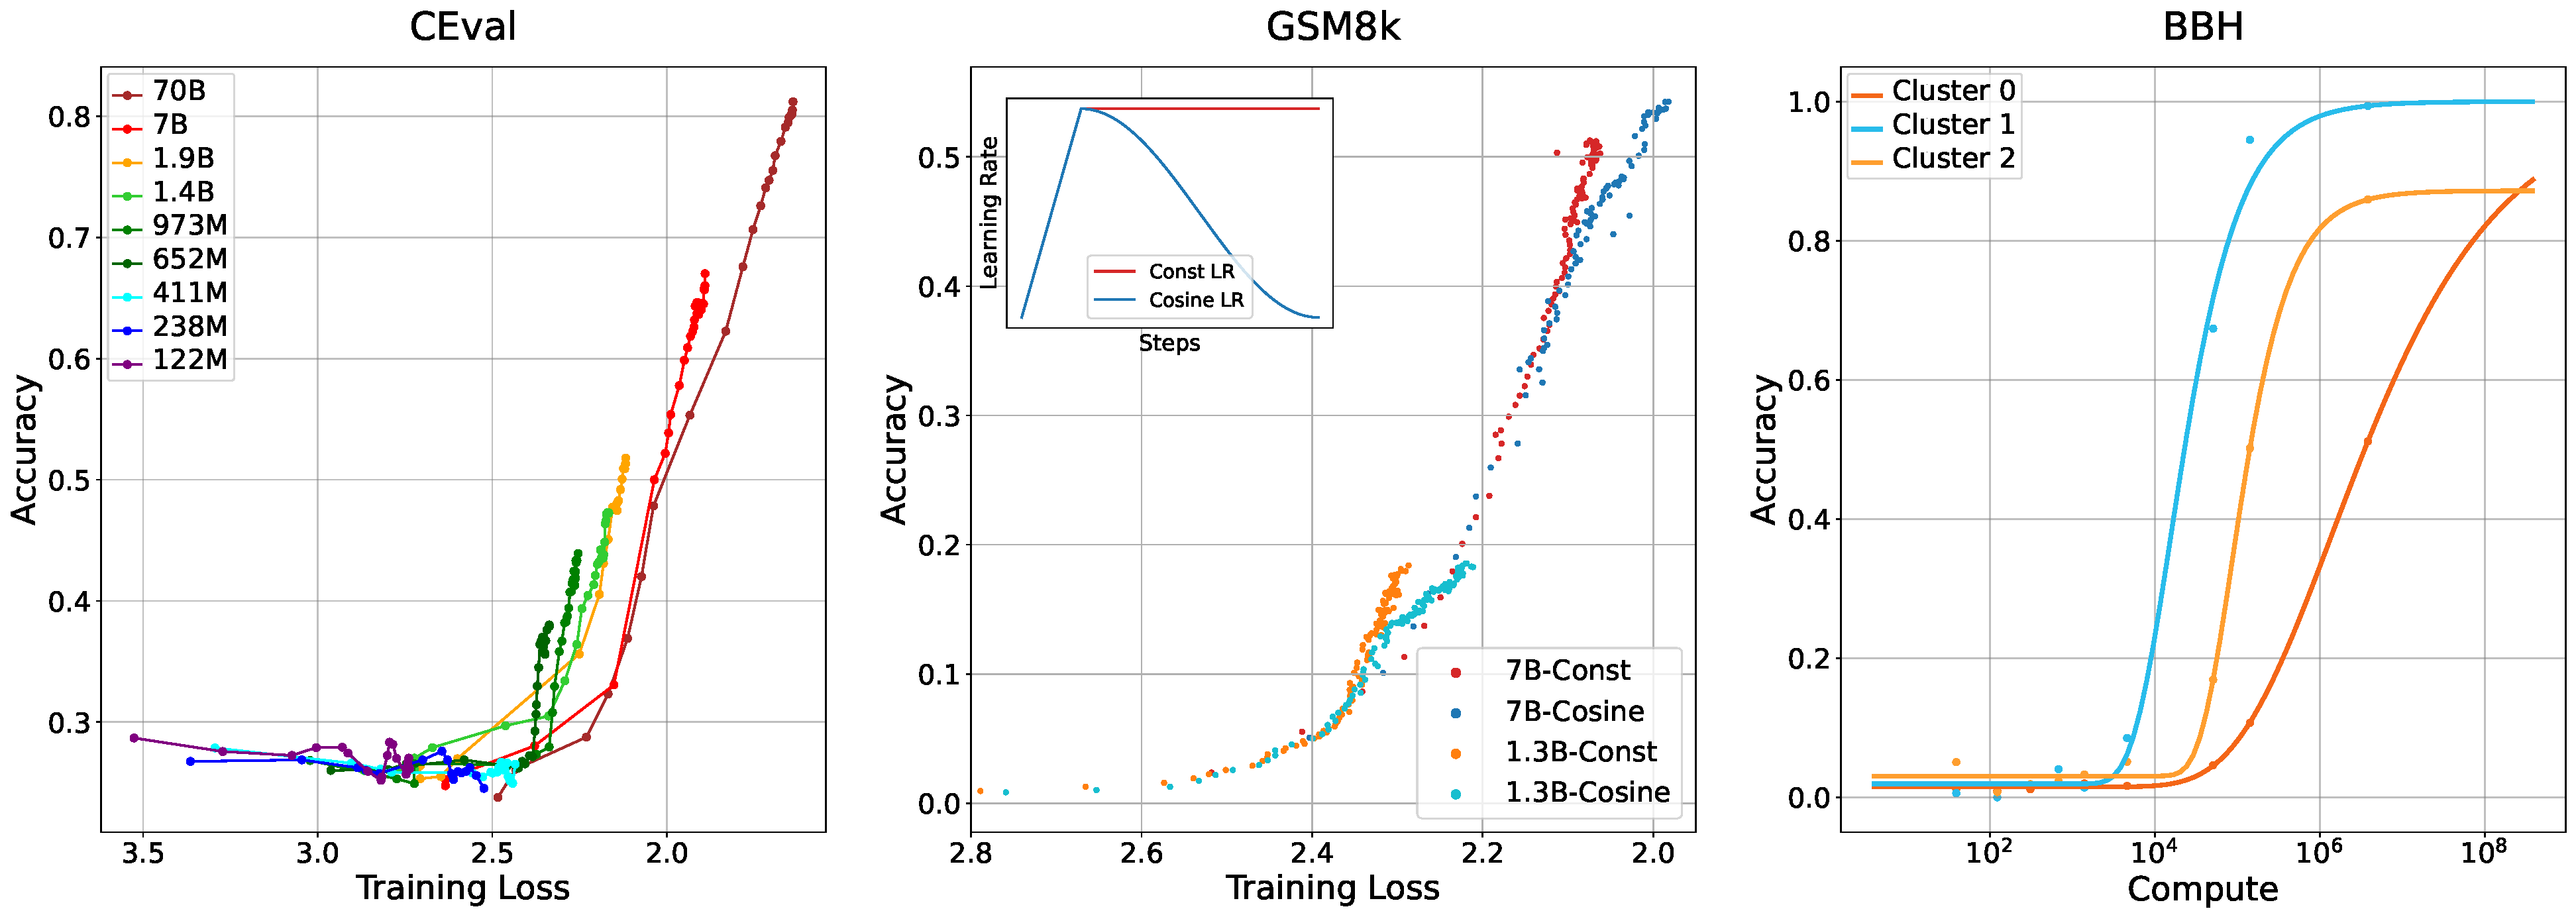
\includegraphics[width=\linewidth]{figures/related_works/ff_gsm8k_cot_v1_avg_score_loss_perf.pdf}
    \caption{Performance-loss relationship across different model sizes (left) and learning rate schedules (middle). Performance-compute relationship for different clusters of the BBH samples(right)}
    \label{fig:perf-loss}
    \vspace{-14pt}
\end{figure*}
In this section, we present the pilot experiments to illustrate the shortcomings of existing approaches. 

\noindent\textbf{Training loss may mismatch downstream task performance.}
Predicting downstream performance from training loss assumes LLMs achieve identical downstream results at the same loss value, which does not hold universally.
%
In practice, training loss primarily serves as an indicator of in-domain fitting, whereas downstream tasks typically represent out-of-domain evaluations. Moreover, training configurations, such as model size and learning rate, can significantly affect not only the final loss but also the model’s generalization capabilities.


\cref{fig:perf-loss}(left) illustrates the performance–loss relationships for LLMs of different sizes on the CEval benchmark~\citep{nguyen2024ceval}. At the same training loss level, smaller models can outperform larger ones in terms of test accuracy. Because smaller models initially exhibit weaker in-domain fitting capacity, they typically require more training steps to reach the same loss value, which can lead to better in-domain generalization once they do. \cref{fig:perf-loss}(middle) compares the performance of LLMs trained under different learning rate schedules on the GSM8k dataset~\citep{cobbe2021training}. At the same loss level, the performance under the cosine schedule is always worse than that under the constant schedule, indicating that a lower learning rate may prioritize memorization over generalization, thereby diminishing downstream performance.

\noindent\textbf{Diverse scaling patterns within the evaluation set.}
Different task samples exhibit unique computational thresholds, learning slopes, and upper bounds, making it challenging to find a single fitting function (or function group) that generalizes well across diverse task samples. \cref{fig:perf-loss}(right) illustrates the performance-compute relationships \revise{on three clusters randomly selected from those formed by clustering tasks based on their difficulty in the BBH benchmark.}~\citep{suzgun2023challenging}, with each cluster containing samples with similar difficulty. Even within a single evaluation set, these scaling curves can vary significantly, indicating that a one-size-fits-all performance-compute curve is insufficient for capturing the full spectrum of a downstream evaluation set.

Taken together, these observations highlight the importance of modeling the heterogeneous scaling properties within an evaluation set and identifying a robust intermediate metric to serve as a reliable indicator of the downstream performance of LLMs.
% \begin{figure*}[t]
%   \includegraphics[width=0.48\linewidth]{example-image-a} \hfill
%   \includegraphics[width=0.48\linewidth]{example-image-b}
%   \caption {A minimal working example to demonstrate how to place
%     two images side-by-side.}
% \end{figure*}

\begin{figure*}[t]
    \centering
    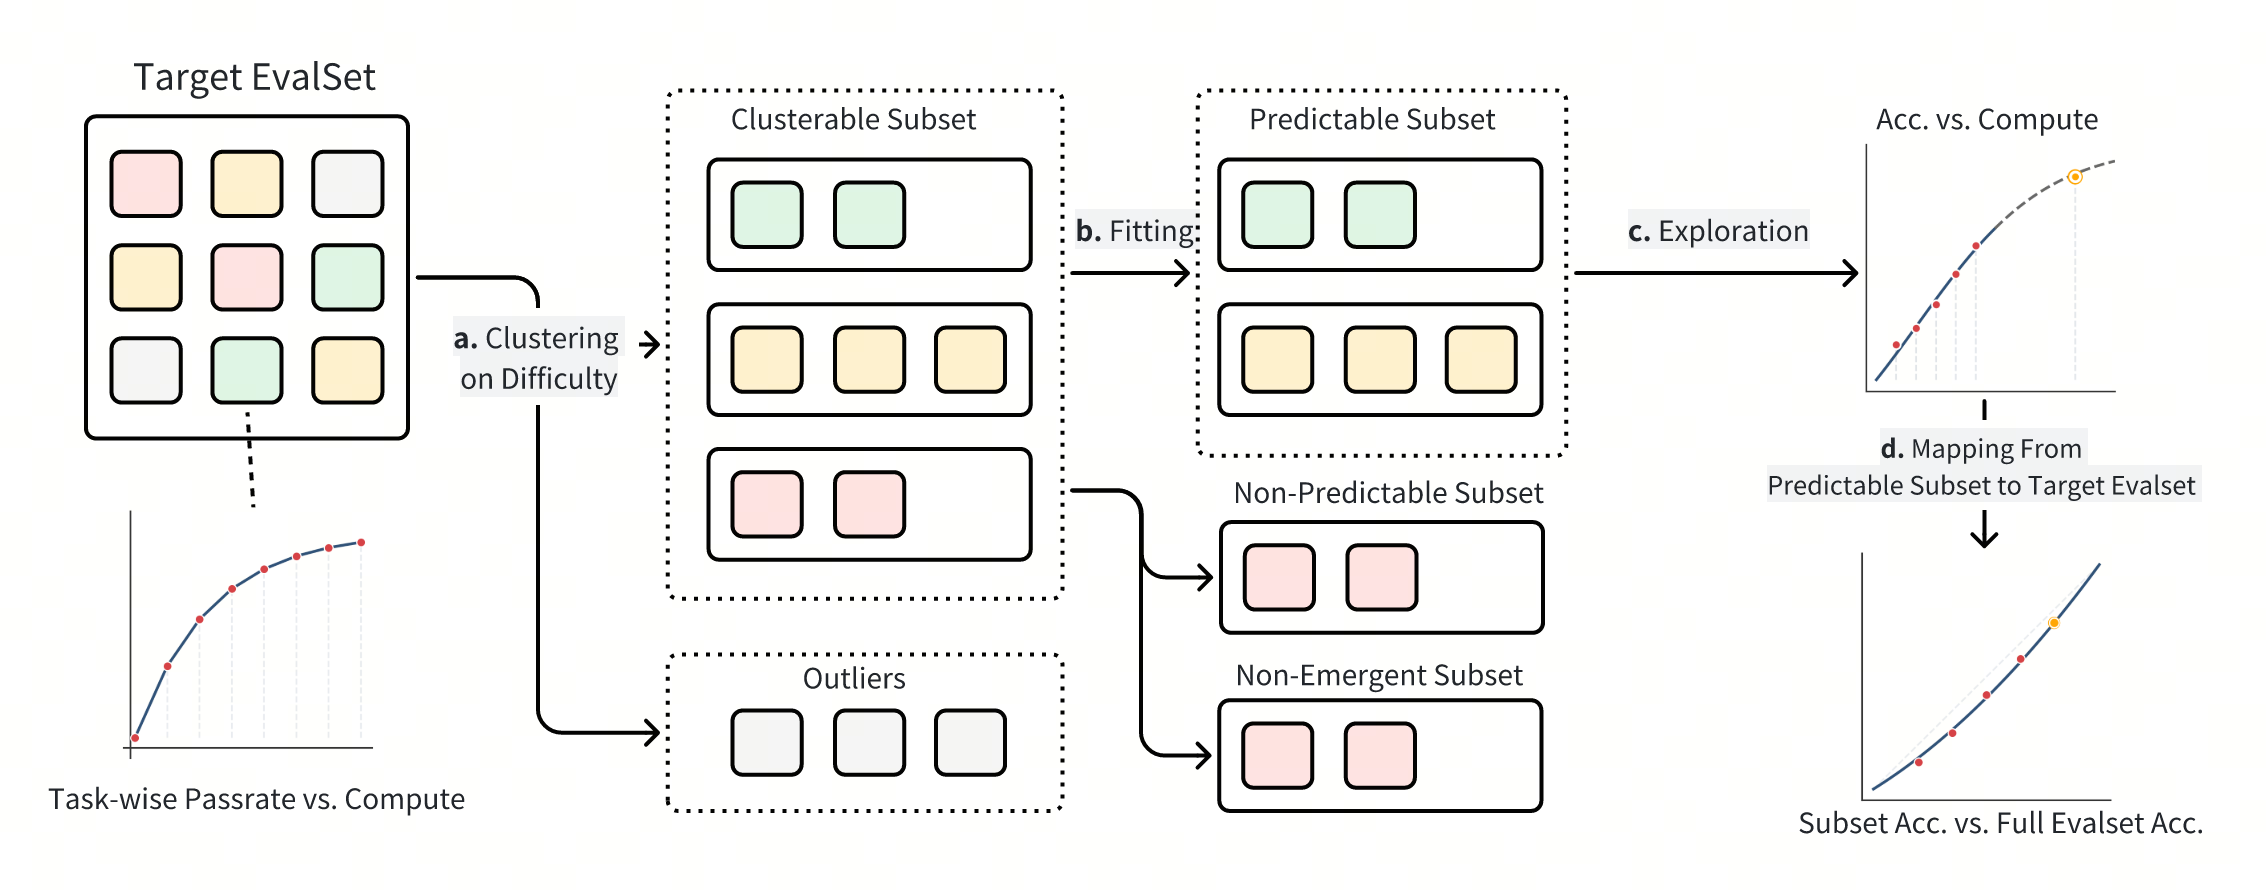
\includegraphics[width=\linewidth]{figures/method/MainPipeline.png}
    \vspace{-15pt}
    \caption{The pipeline of Cluster-On-Difficulty downstream task performance scaling, including 4 stages: \textbf{a}. Represent task difficulty feature with task-wise passrate vector. Cluster on the difficulty feature and filter outliers. \textbf{b}. Fit cluster-wise performance-compute curve. Classify clusters into extrapolatable clusters, non-extrapolatable clusters, and non-emergent clusters. \textbf{c}. Predict accuracy on extrapolatable clusters. \textbf{d}. Map subset accuracy prediction to full evaluation set performance.}
    \label{fig:main-pipeline}
    \vspace{-7.5pt}
\end{figure*}



\vspace{-7pt}
\section{Method}
\vspace{-5pt}
\label{sec:method}

In this section, we first formulate the problem, then present COD in four stages (see \cref{fig:main-pipeline}).
(1) We construct sample-level difficulty scaling features and apply an improved MeanShift clustering algorithm (\cref{sec:method-clustering}).
(2) We derive a performance scaling law with respect to task difficulty variance, enabling extrapolation of performance–compute relationships for clusters with similar difficulty features. Cluster-wise curves are fitted on small models to identify extrapolatable clusters (\cref{sec:fitting}).
(3) We extrapolate performance for these clusters to predict the target large model’s accuracy on the predictable subset (\cref{sec:extrapolation}).
(4) Finally, we map subset accuracy to full evaluation results (\cref{sec:mapping}).

\textbf{Problem Formulation.} Consider a language model $M_C$ trained with a compute budget of $C$ measured in FLOPs. Let $\mathcal{P}$ be a set of downstream tasks that we aim to evaluate the model on. Each sample $T \in \mathcal{P}$ is defined by a question-answer pair $(q, a_{\text{true}})$. Given a question $q$, the model $M_C$ outputs a probability distribution $p(a|q; M_C)$ over the space of all possible answers.

% \labubu{For a task instance $(q, a_{\text{true}})$ where the answer is a token sequence $a_{\text{true}} = (t_1, t_2, \ldots, t_k)$, the Next-Token-Prediction loss $L(q, a_{\text{true}}; C)$ is defined as the sum of the negative log-probabilities of the ground-truth tokens:}

% $$L(q, a_{\text{true}}; C) = -\sum_{i=1}^{k} \log p(t_i | q, t_{<i}; M_C)$$

Our goal is to predict the downstream task performance of a large language model $M_{C_{\text{target}}}$ using only evaluation results from smaller models $\{M_{C_1}, M_{C_2}, \ldots, M_{C_n}\}$ where $C_i \ll C_{\text{target}}$ for all $i$. Formally, we aim to find the prediction method $\phi$ to minimize the absolute prediction error over a group of tasks sets $\{\mathcal{P}_j\}_m$:
$$\arg\min_{\phi}\frac{1}{m}\sum_{i=1}^m\frac{1}{|\mathcal{P}_j|}\sum_{T\in \mathcal{P}_j}\vert\widehat{\text{Acc}}(C_{\text{target}}, T)-\text{Acc}(C_{\text{target}})\vert,$$
$$\widehat{\text{Acc}}(C_{\text{target}}, T) := \phi\left(\{\text{Acc}(C_i, T)\}_{i=1}^{n}, \{C_i\}_{i=1}^{n}, C_{\text{target}}\right),$$
where $\text{Acc}(C, T)$ denotes the accuracy of model $M_C$ on task $T$, and $\widehat{\text{Acc}}(C_{\text{target}}, T)$ is the predicted accuracy for the target model.


\subsection{Clustering on Difficulty}
\label{sec:method-clustering}

\camera{Although downstream tasks in the same evaluation set share similar themes, they exhibit significant differences in difficulty, resulting in distinct performance scaling patterns that make a universal fitting function inapplicable.} We propose clustering tasks by similar performance scaling behaviors to minimize intra-cluster heterogeneity maintaining a minimum cluster size.

Specifically, we train a group of language models with increasing parameter counts. These models are trained with the same ratio of training tokens to compute per token. %我们采用和预估阶段相同一组小模型来评测任务的难度特征，不会引入大模型评测结果以避免信息泄露额。
\revise{We use the same set of small models for prediction to evaluate the difficulty characteristics of the task, and will not introduce the target large model evaluation results to avoid feature leakage.}

For each task, we generate 100 samples using \texttt{top\_p}=0.7 and \texttt{temperature}=1.0 for each model, and compute the pass rate by averaging the results. This pass rate serves as an estimate of the model’s expected accuracy on the task. The resulting values are \revise{concatenated} into a difficulty vector, ordered by increasing model size. For most tasks, this difficulty vector exhibits a monotonic increase, reflecting the gradual improvement of model capability with scale.



\begin{figure*}[!t]
    \centering
    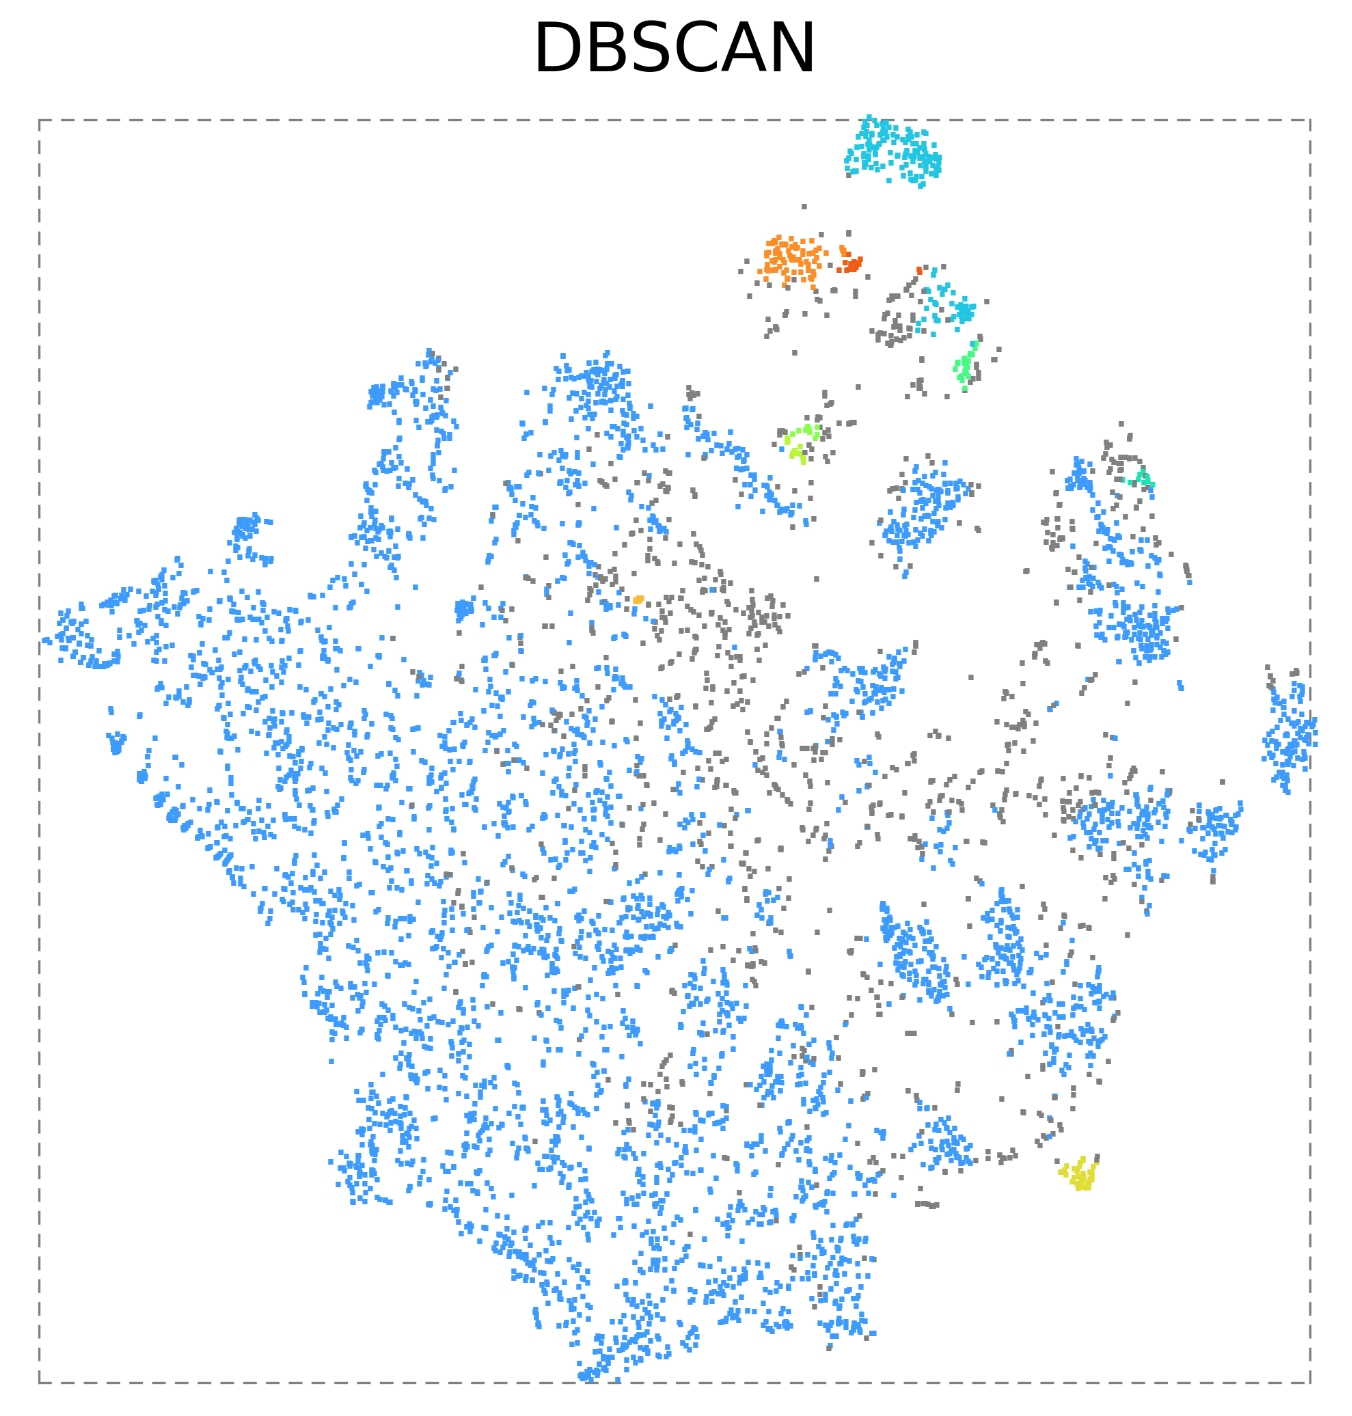
\includegraphics[width=0.28\textwidth]{figures/method/DBSCAN_BBH_v2.jpeg}
    \hspace{0.03\textwidth}  % 调整两图之间的间距
    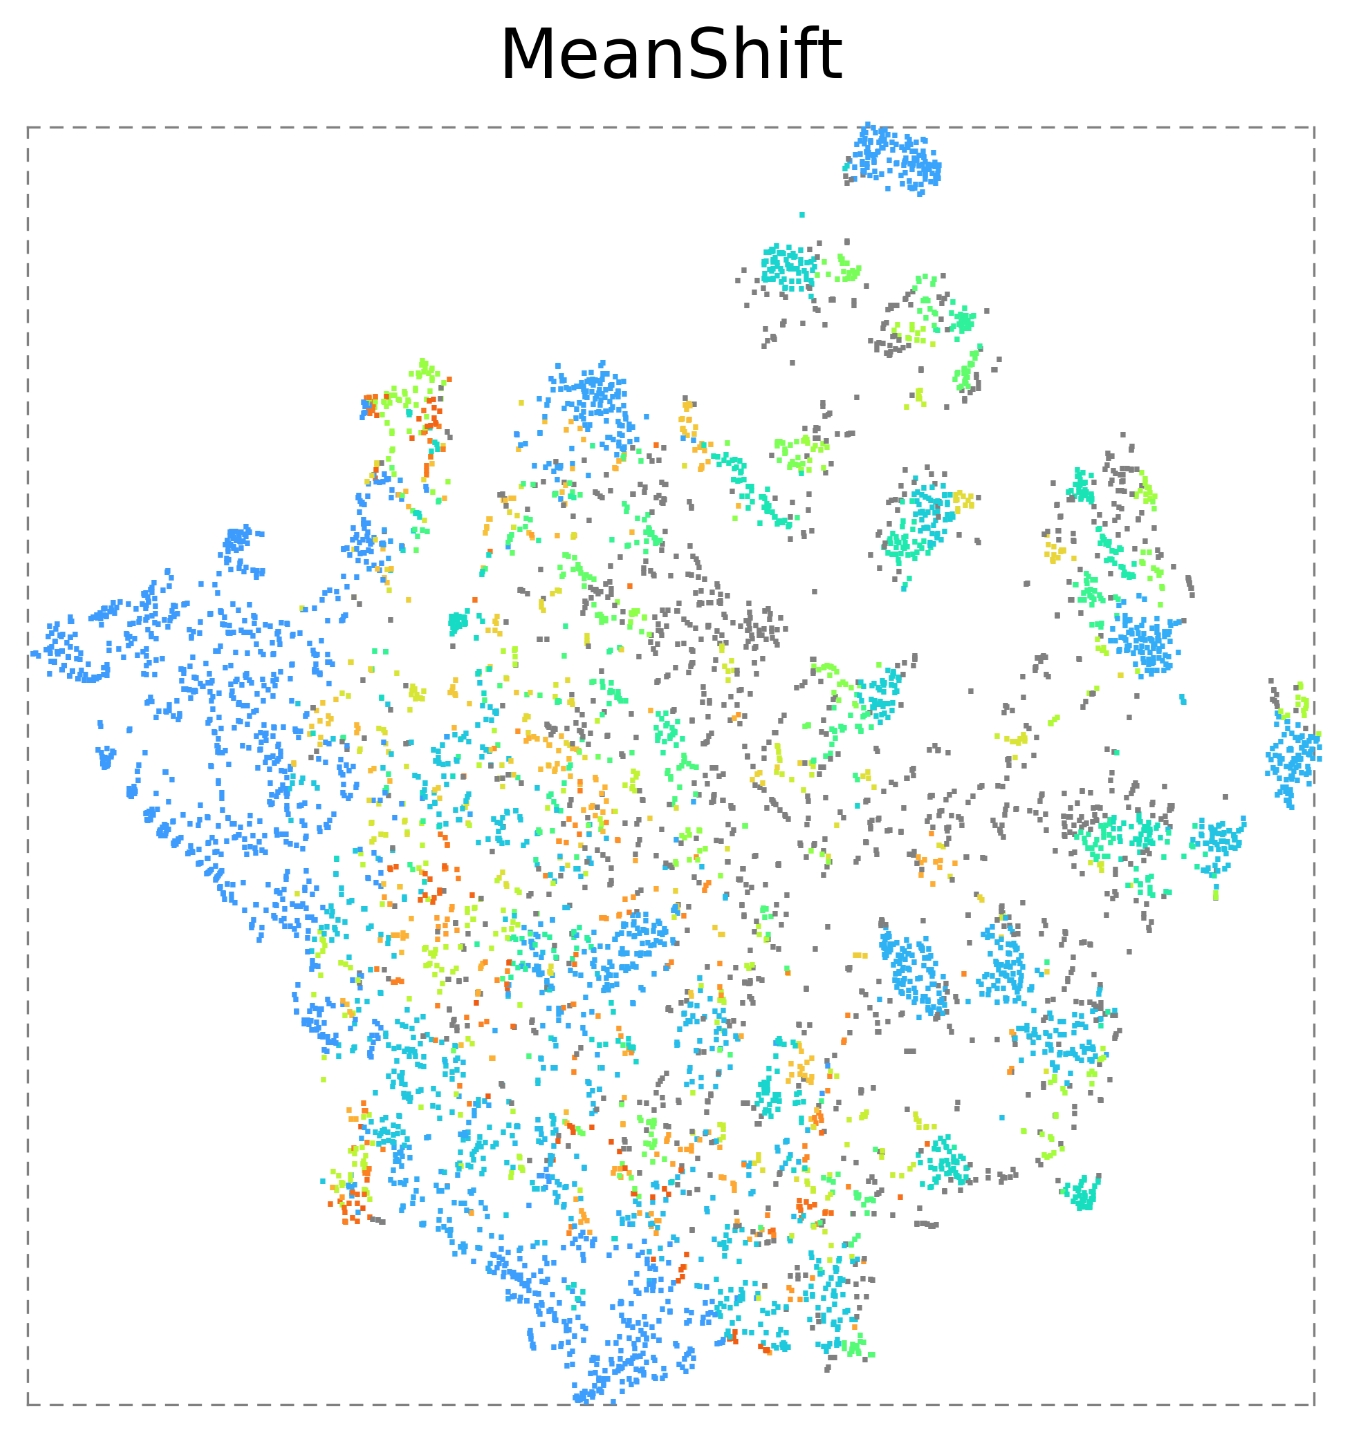
\includegraphics[width=0.28\textwidth]{figures/method/MeanShift_BBH_v2.jpeg}
    \hspace{0.03\textwidth}  % 调整两图之间的间距
    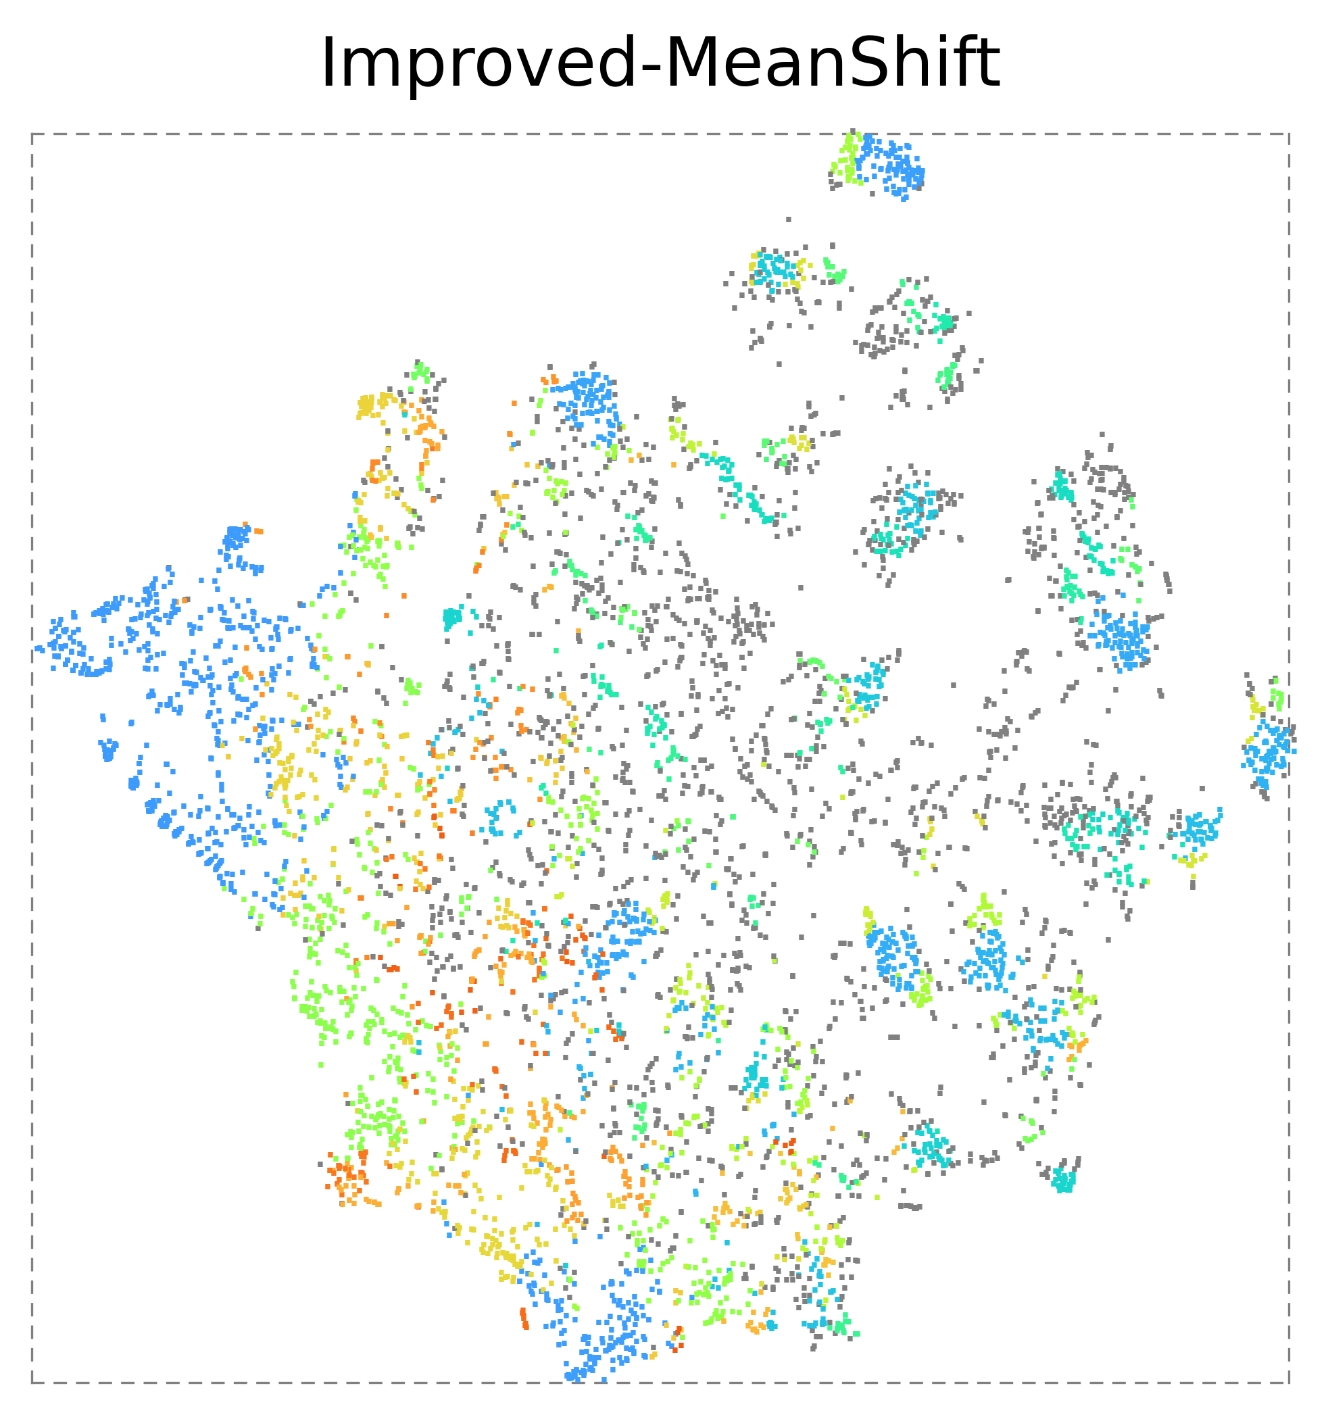
\includegraphics[width=0.28\textwidth]{figures/method/ImprovedMeanShift_BBH_v2.jpeg}
    \caption{t-SNE visualization of different clustering methods: DBSCAN(left), MeanShift(Middle), Improved-MeanShift(Right). Each point represents an evaluation sample. }
\label{fig:tsne_vis}
\vspace{-10pt}
\end{figure*}

After obtaining the difficulty feature vector for each task, we use the improved clustering algorithm that incorporates the following features:
(1) Minimizing intra-class variance to ensure similar extrapolation properties within each cluster;
(2) Automatic determination of cluster numbers, as the optimal number varies across evaluation sets and is difficult to pre-specify. 

% K-Means~\citep{macqueen1967some} requires pre-specifying cluster numbers and DBSCAN~\citep{ester1996density} may yield large intra-cluster variance, MeanShift~\citep{fukunaga1975estimation} allows constraining this variance via a radius parameter, better suiting our needs.

To further reduce intra-class variance, we propose an improved MeanShift algorithm to constrain the cluster diameter. At the same time, we maintain a minimum number of tasks in each cluster to reduce metric fluctuations.
We provide the t-SNE visualization of clustering results evaluation tasks on BBH~\citep{suzgun2023challenging} to compare the proposed method and classic clustering algorithms including DBSCAN~\citep{ester1996density} and MeanShift~\citep{fukunaga1975estimation}. Each point represents an evaluation sample, and its color denotes the cluster type. As shown in \cref{fig:tsne_vis}, our improved MeanShift effectively splits dense areas whereas DBSCAN and the original MeanShift produce connected clusters with large within-cluster distances.

We provide numerical comparison of clustering algorithms in~\cref{sec:clustering_ablation} and explain implementation details of improved MeanShift in Appendix~\ref{sec:improved},  smoothing techniques in Appendix~\ref{sec:smoothing}. 

% We also cast an ablation study on clustering methods in \cref{sec:clustering_ablation}.


\subsection{Fitting}
\label{sec:fitting}
% 得到聚类结果后，我们在每个类簇上计算评估指标，并完成独立的外推曲线拟合。
% 我们给出Scaling Law for Downstream Task Performance以及对应的理论分析, 并可以从中推导出难度特征相似的类簇上的Performance scaling预测公式。

After clustering, we compute metrics for small models within each cluster.
\camera{We then fit the accuracy-compute curves for each cluster using a theoretically derived novel performance scaling law}, focusing on clustered samples after excluding outliers. We derive the following fitting formula for the downstream task scaling law based on the training loss scaling law.


\begin{theorem}[Scaling Law for Downstream Task Performance]
\label{main:proof:task_scaling_law}
Consider a language model $M_C$ trained with compute budget $C$ and a set of downstream tasks $\mathcal{P}$. Under the following assumptions:
Assumption 1 (Power-law scaling of answer loss): the expected answer loss follows:
\begin{equation}
L_{\mathcal{P}}(C) := \mathbb{E}_{(q,a_{\text{true}}) \sim \mathcal{P}}[L(q, a_{\text{true}}; C)] = \alpha C^{-\beta} + \gamma,
\end{equation}
where $\alpha, \beta, \gamma > 0$ are task-specific constants, with $\gamma$ representing the irreducible loss.

Assumption 2 (Unique deterministic answers): Each question has a unique deterministic answer. The model receives score $1$ if and only if $M_C$ outputs $a_{\text{true}}$, and $0$ otherwise.

Assumption 3 (Accuracy decomposition): The expected accuracy decomposes as:
\begin{equation}
\mathbb{E}_{T \sim \mathcal{P}}[\mathrm{Acc}(C)] = g + (1-g) \cdot \mathbb{E}_{(q,a_{\text{true}}) \sim \mathcal{P}}[p(a_{\text{true}}|q, M_C)],
\end{equation}
where $g \in [0,1]$ is the random guessing baseline.

Then, the expected accuracy on task set $\mathcal{P}$ can be modeled as:
\begin{equation}
\mathbb{E}_{\mathcal{P}}[\mathrm{Acc}(C)] =g+(1-g)\left(\exp{(-\alpha C^{-\beta}-\gamma)} + \frac{\sigma_L^2(C)}{2\mu_L(C)} \right)+ o\left(\sigma_L^2(C)\right), 
\end{equation}
where $\mu_L(C) = \mathbb{E}_{(q,a_{\text{true}}) \sim \mathcal{P}}[L(q, a_{\text{true}}; C)]$ is the mean loss and $\sigma_L^2(C) = \mathrm{Var}_{(q,a_{\text{true}}) \sim \mathcal{P}}[L(q, a_{\text{true}}; C)]$ is the loss variance across the task set.
\end{theorem}


\begin{proof}[Proof Sketch]
By definition of the language model loss, $p(a_{\text{true}}|q, M_C) = \exp(-L(q, a_{\text{true}}; C))$. Under Assumption 1, if the answer loss follows a power law $L \sim \alpha C^{-\beta} + \gamma$, then the task passrate should approximately scale as $\exp(-\alpha C^{-\beta} - \gamma)$.

The key subtlety lies in the averaging: accuracy computes $\mathbb{E}[\exp(-L)]$ (arithmetic mean of passrates) while the loss scaling law gives us $\exp(-\mathbb{E}[L])$ (geometric mean). Using Taylor expansion:
$$\mathbb{E}[\exp(-L)] \approx \exp(-\mu_L) \ + \frac{\sigma_L^2}{2\mu_L},$$
where $\mu_L$ and $\sigma_L^2$ are the mean and variance of the loss distribution.

This approximation is accurate when tasks have similar difficulty feature ($\sigma_L^2/\mu_L^2 \ll 1$), motivating our clustering approach to reduce intra-cluster variance. Assumption 3 adds the parameter $g$ for random guessing. The complete proofs are provided in Appendix~\ref{sec:prop_proof}.
\end{proof}
\cref{main:proof:task_scaling_law} demonstrates that a metric of an evaluation set with similar difficulty features can be effectively modeled using the following formula:
\begin{equation}
y(C)=g+(1-g)*e^{-aC^{-b}-c},
\label{eq:fitting}
\end{equation}
where $a$ and $b$ jointly influence how accuracy varies with $C$, while $c$ constrains the upper bound of the fitting curve, and $g$ represents the expected random guess metric for a task cluster. 
$a$, $b$, $c$, and $g$ are trainable parameters. 
Note that these assumptions may not perfectly hold in practice, we provide additional discussions on assumption 3 in Appendix~\ref{sec:limiations}.


\subsection{Extrapolation}
\label{sec:extrapolation}

To ensure reliable extrapolation, we identify clusters exhibiting robust scaling patterns, as some clusters may show saturated or non-emergent performance on smaller models, making them unsuitable for prediction. We aim to find an extrapolation subsets that represent the full set performance, and use the subset metric as a intermediate indicator for the prediction of the full set accuracy.

A cluster is deemed \textbf{extrapolatable} if it meets two criteria: (1) its expected accuracy increases monotonically with model size, and (2) its performance converges to at least a predefined threshold~$P$ (where $P \leq 1$ accounts for practical limits like ambiguous questions or finite training coverage). 

We filter out non-extrapolatable clusters using two rules based on the parameters from \cref{eq:fitting}:
\begin{enumerate}[leftmargin=1.5em]
    \item Negligible accuracy growth, indicated by minimal $a$ or $b$ values.
    \item Poor extrapolation reliability, indicated by an excessive $c$ value.
\end{enumerate}
In practice, for extrapolatable clusters, we set $a > 1$, $b > 0.1$, and $0 \leq c < 1$. \anno{Further ablation experiments are provided in Appendix~\ref{sec:criteria}.}

The clusters satisfying these conditions form the \textit{predictable subset}. The final performance prediction for a target model on this subset is the weighted average of the extrapolated predictions from these individual clusters, with weights proportional to cluster sizes.

% \subsection{Mapping from Predictable Subset to Target Evaluation Set}
% \label{sec:mapping}
% We map predictions from the predictable subset $\mathcal{P}'$ to the complete evaluation set $\mathcal{P}$ using a \camera{smooth} function. This approach is based on the observation that extrapolatable and non-extrapolatable samples, while differing in difficulty, often share question types, suggesting a preserved relative metric ordering. The mapping function $f: \text{Acc}(\mathcal{P}') \rightarrow \text{Acc}(\mathcal{P})$ is continuous, smooth over $[0,1]$, monotonically increasing, and constrained to pass through $(0,0)$ and $(1,1)$. Empirical validation indicates a polynomial function optimally captures this relationship:
% \begin{equation}
%     f_n(x)=\alpha_{n-1}x^n+\alpha_{n-2}x^{n-1}+...+\alpha_1x^2+(1-\alpha_1-\alpha_2-...-\alpha_{n-1})x,
%     \label{eq:mapping}
% \end{equation}
% \anno{where $x$ represents the average accuracy of the predictable subset $\mathcal{P}'$, and 
% $n$ denotes the highest degree of the polynomial. In practical implementation, a quartic function is employed to fit the mapping (see Appendix~\ref{sec:interpolation_ablation} for exhaustive experimental details).} To ensure reliability, we calibrate $f$ using evaluation results from existing models as anchors. This subset-to-full mapping generally demonstrates robustness across diverse model architectures and training data, often permitting the use of external models (e.g., Qwen2-72B~\citep{yang2024qwen2}) as anchors for many tasks (see Appendix~\ref{sec:anchor} for experiments). However, for data-sensitive tasks, models with similar training distributions provide more reliable anchors, prioritizing data consistency for mapping accuracy. The final metric prediction for a target LLM with estimated training computation $C_0$ is then $p = f \circ y(C_{0})$, combining the cluster-wise extrapolation $y(C_0)$ from \cref{eq:fitting} with the mapping $f$.

\camera{\subsection{Mapping from Predictable Subset to Target Evaluation Set}
\label{sec:mapping}
We map predictions from the predictable subset $\mathcal{P}'$ to the complete evaluation set $\mathcal{P}$ using a smooth function. This mapping strategy is motivated by the observation that extrapolatable and non-extrapolatable samples, despite their difficulty differences, usually belong to the same question types, which implies a consistent relative metric ordering between the predictable subset and the full evaluation set. The mapping function $f: \text{Acc}(\mathcal{P}') \rightarrow \text{Acc}(\mathcal{P})$ is continuous, smooth over $[0,1]$, monotonically increasing, and constrained to pass through $(0,0)$ and $(1,1)$. Empirical validation indicates that a smoothing spline optimally captures this relationship. Specifically, we employ a cubic smoothing spline to model the mapping.
where $x$ represents the average accuracy of the predictable subset $\mathcal{P}'$. In practical implementation, under the premise of fixing the curve to pass through $[0,0]$ and $[1,1]$, we determine the number of piecewise cubic segments (knots) by setting a Root Mean Square Error (RMSE) fitting threshold of $0.005$. The number of segments is dynamically adjusted until the fitting RMSE meets this threshold. 
We list the implementation details and visualization of mapping in \cref{sec:interpolation_ablation}.

To ensure reliability, we calibrate $f$ using evaluation results from existing models as anchors. This subset-to-full mapping generally demonstrates robustness across diverse model architectures and training data, often permitting the use of external models (e.g., Qwen2-72B~\citep{yang2024qwen2}) as anchors for many tasks (see Appendix~\ref{sec:anchor} for experiments). The final metric prediction for a target LLM with estimated training computation $C_0$ is then $p = f \circ y(C_{0})$, combining the cluster-wise extrapolation $y(C_0)$ from \cref{eq:fitting} with the mapping $f$.}


\vspace{-5pt}
\section{Experiments}
\label{sec:expr}
\vspace{-5pt}
\subsection{Experimental Setups}
\label{sec:exp_setups}

In our experimental setup, \anno{we train nine language models ranging from 122M to 70B parameters in total, which share the same data distribution and architecture, with the training data scaled proportionally to their sizes.} We show the detailed training configurations and recipe in Appendix~\ref{append:setting}.

% \noindent\textbf{Downstream evaluation sets.}
For evaluation, we adopt the following widely used benchmarks, including GSM8K \citep{cobbe2021training}, MATH \citep{hendrycks2021measuring}, BBH \citep{suzgun2023challenging}, TriviaQA \citep{joshi2017triviaqa},
MBPP \citep{austin2021program}, AGIEval \citep{zhong2023agieval},
DROP \citep{dua2019drop}, MMLU-pro \citep{wang2024mmlu}. 
All models are evaluated in a few-shot in-context learning manner, and we aligned our evaluation setups with LLaMa3~\citep{dubey2024llama}.We evaluate the proposed COD performance scaling for LLMs against existing approaches on multiple public benchmarks. Using eight smaller language models as known information, we estimate the downstream task performance of a pretrained LLM with 70B parameters. 

\subsection{Prediction Experiments}
\label{subsec:Prediction_Experiments}
We compare COD against four representative prediction methods:
\begin{enumerate}[leftmargin=2em]
\item Loss-intermediate~\citep{chen2024scaling}: First predicts the target LLM's final training or validation loss, then estimates downstream task metrics based on the relationship between smaller models' evaluation metrics and their losses.
\item \camera{End-to-end(exp)}~\citep{xiao2024densing}: Directly extrapolates large model metrics from smaller model evaluation set metrics using \camera{exponential-based} performance scaling laws.
\item \camera{End-to-end(passrate)}~\citep{achiam2023gpt,hu2023predicting}: A variant of end-to-end method, which estimates large model passrates from smaller model passrates. We conduct 100 trials per evaluation set for smaller models to enhance reliability and report absolute prediction error on the passrate metric.
\item \camera{End-to-end(BNSL)}~\citep{caballero2022broken}: Decomposes the end-to-end mapping into a multi-segment power-law framework.
\end{enumerate}

\begin{table*}[!t]
\small
\setlength{\tabcolsep}{1.8pt} % Keep this if column spacing is critical
\centering
\caption{Absolute prediction error (\%) on evaluation sets for predicting the performance of the 70B model. Errors < 2\% are considered accurate (green), while errors > 5\% are considered invalid (red). $\downarrow$ indicates lower is better.}
\begin{tabular}{c|cc|cccccccc}
\toprule
\multirow{2}{*}{Method} & \multicolumn{2}{c|}{Overall Metrics} & \multicolumn{8}{c}{Individual Task Sets} \\
\cmidrule(lr){2-3} \cmidrule(lr){4-11}
& Mean$\downarrow$ & Max$\downarrow$ & GSM8k & MATH & BBH & TriviaQA & MBPP & AGIEval & DROP & MMLU-pro \\
\midrule
Loss-intermediate & 5.29 & 9.39 & \redhl{9.39} & \redhl{6.95} & 2.33 & \redhl{5.81} & \redhl{5.52} & \greenhl{1.41} & \redhl{5.37} & \redhl{5.55} \\
End-to-end\camera{(exp)} & 3.10 & 6.00 & 4.00 & 3.86 & \greenhl{0.64} & \greenhl{0.68} & \greenhl{1.75} & \redhl{6.00} & 4.11 & 3.72 \\
\camera{End-to-end(passrate)} & 5.02 & 8.80 & \redhl{6.71} & \redhl{8.80} & 3.51 & 4.00 & \redhl{7.34} & \redhl{6.78} & \greenhl{0.26} & 2.74 \\
\camera{End-to-end(BNSL)} & 5.17 & 13.05 & 4.23 & \redhl{5.88} & \redhl{13.05} & \redhl{5.86} & 2.55 & \greenhl{0.82} & \greenhl{1.53} & \redhl{7.42} \\
\midrule
COD (w/o mapping) & 2.24 & 5.26 & 4.70 & \greenhl{0.50} & 2.91 & \greenhl{1.98} & \greenhl{0.89} & \redhl{5.26} & \greenhl{1.08} & \greenhl{0.57} \\
% COD (Complete) & \textbf{1.63} & \textbf{2.38} & 2.23 & \greenhl{1.28} & \greenhl{1.77} & \greenhl{1.64} & 2.19 & 2.38 & \greenhl{0.23} & \greenhl{1.35} \\
COD (Complete) & \textbf{1.55} & \textbf{2.68} & 2.68 & \greenhl{0.79} & \greenhl{0.47} & \greenhl{1.97} & 2.42 & \greenhl{1.64} & \greenhl{1.05} & \greenhl{1.39} \\
\bottomrule
\end{tabular}
\label{tab:baseline_comparison}
\vspace{-10pt}
\end{table*}

We also evaluate two variants of our COD approach to validate the benefits of its components:
\begin{enumerate}[leftmargin=2em]
    \item COD (w/o mapping): Performs difficulty-based KMeans clustering, extrapolates per cluster, and aggregates metrics without subset-to-full mapping.
    \item COD (Complete): Our full proposed multi-stage approach, including clustering, predictable cluster filtering, subset extrapolation, and subset-to-full mapping.
\end{enumerate}

Comparative results are shown in \cref{tab:baseline_comparison}. Prediction accuracy is measured by the absolute error between predicted and actual performance. We report mean and max prediction errors across all evaluation sets, as well as errors for individual sets. Our complete COD approach significantly outperforms existing methods in both mean (\camera{1.55\%}) and maximum (\camera{2.68\%}) prediction errors, offering reliable guidance for large model training. \camera{Although baseline methods achieve acceptable performance on partial datasets, their large prediction errors on other datasets severely compromise their overall reliability.}
% While baselines perform well on some sets, their substantial errors on others undermine overall credibility.

\begin{figure}[!t]
\vspace{-5pt}
    \centering
    % Assuming minipage setup is for layout, keeping it.
    \begin{minipage}{0.24\textwidth}
        \centering
        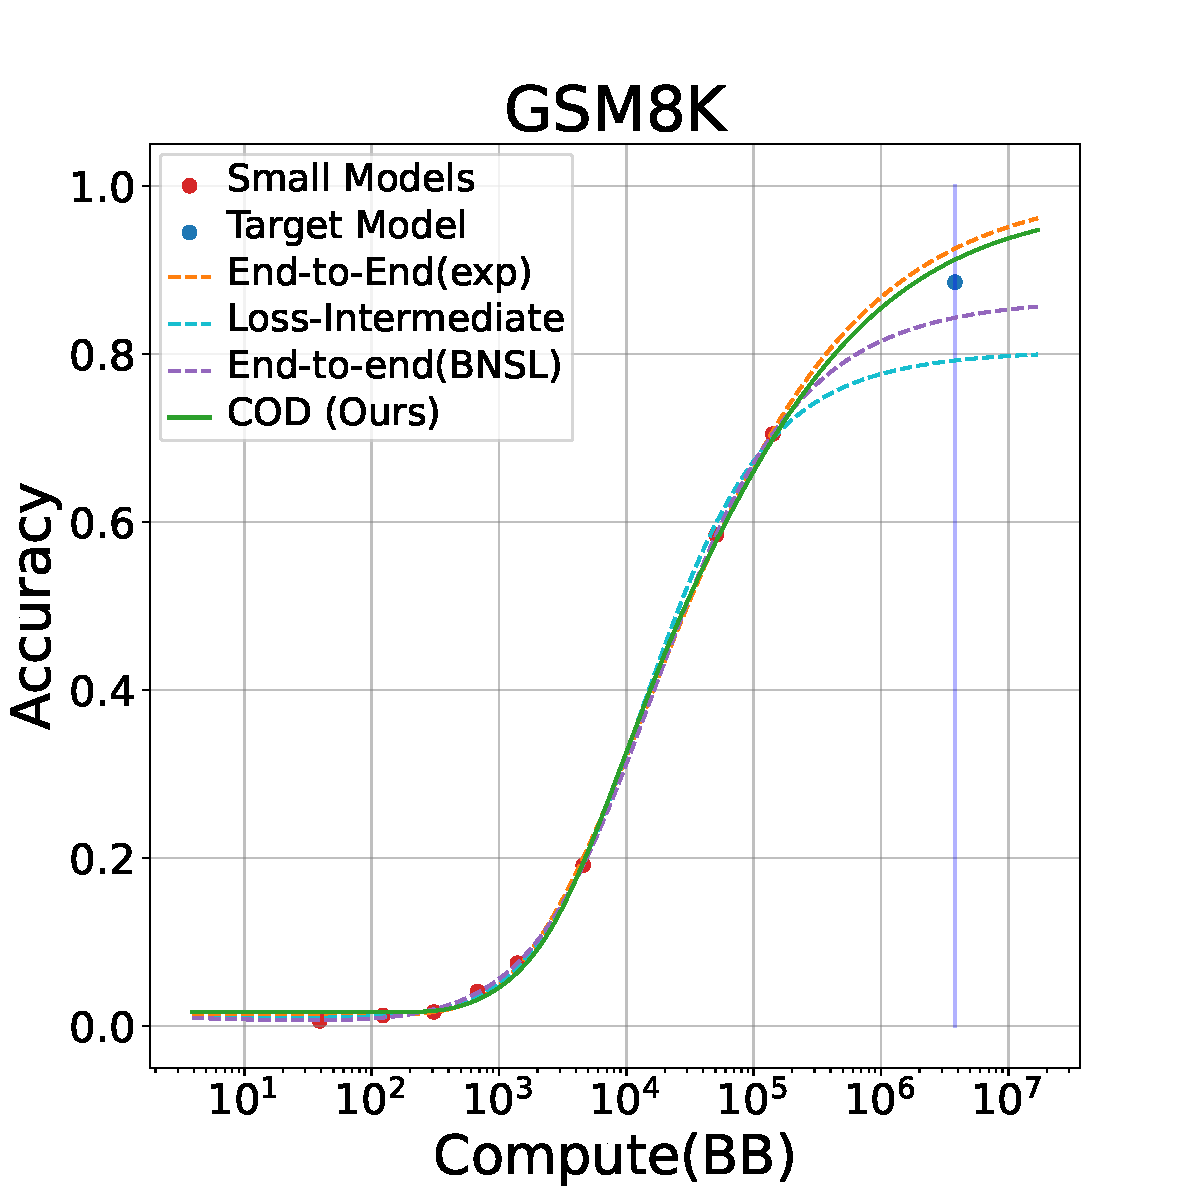
\includegraphics[width=\textwidth]{figures/experiments/perf_compute/GSM8K.pdf}
    \end{minipage}
    \begin{minipage}{0.24\textwidth}
        \centering
        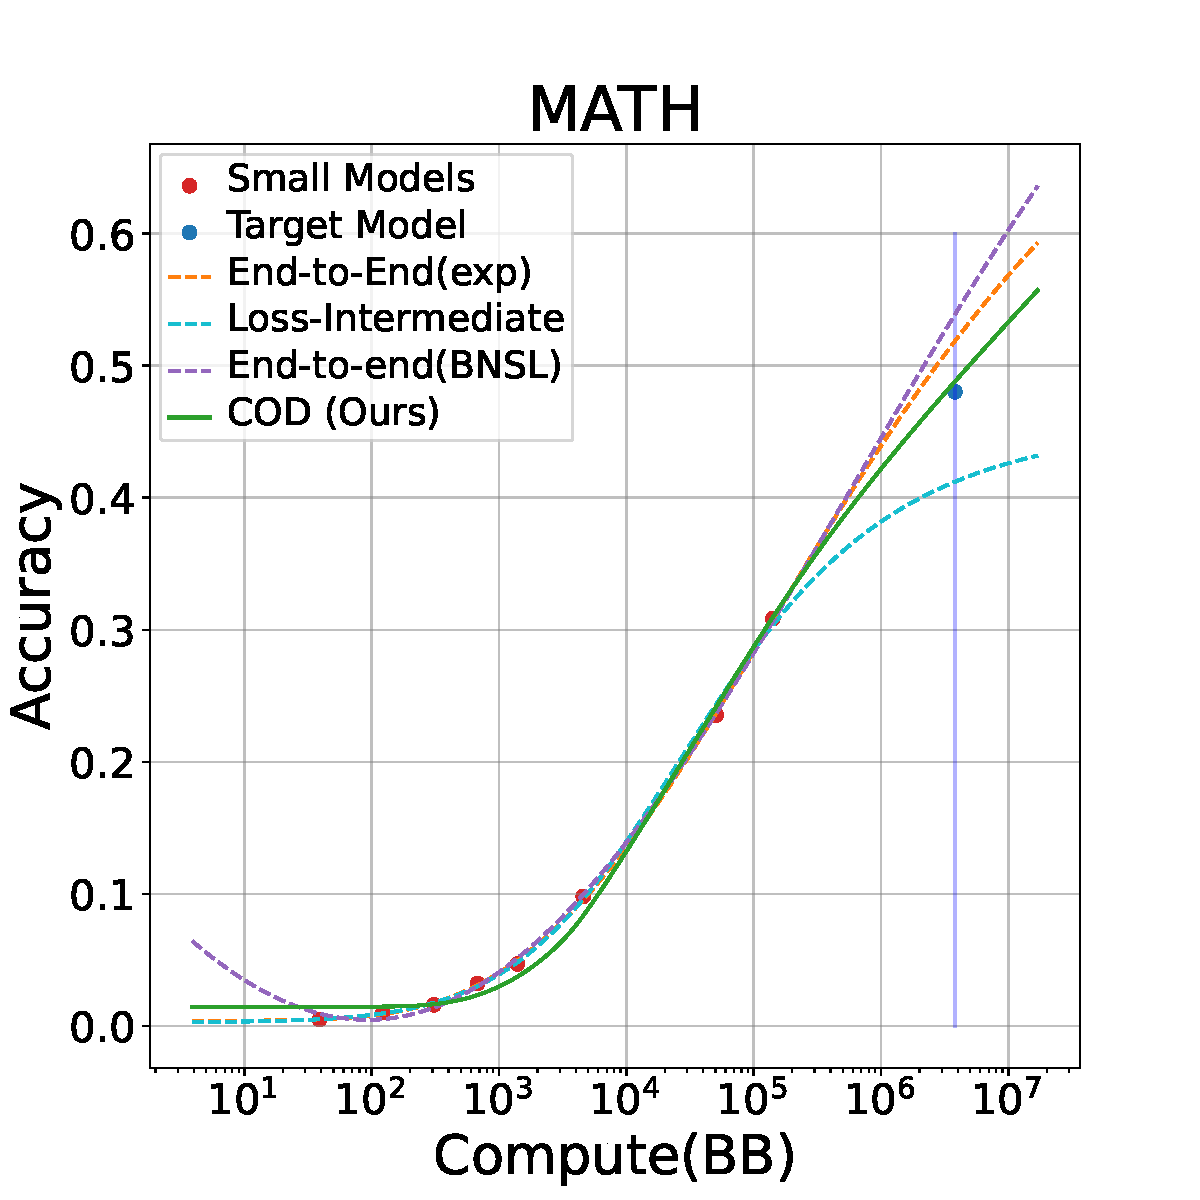
\includegraphics[width=\textwidth]{figures/experiments/perf_compute/MATH.pdf}
    \end{minipage}
    \begin{minipage}{0.24\textwidth}
        \centering
        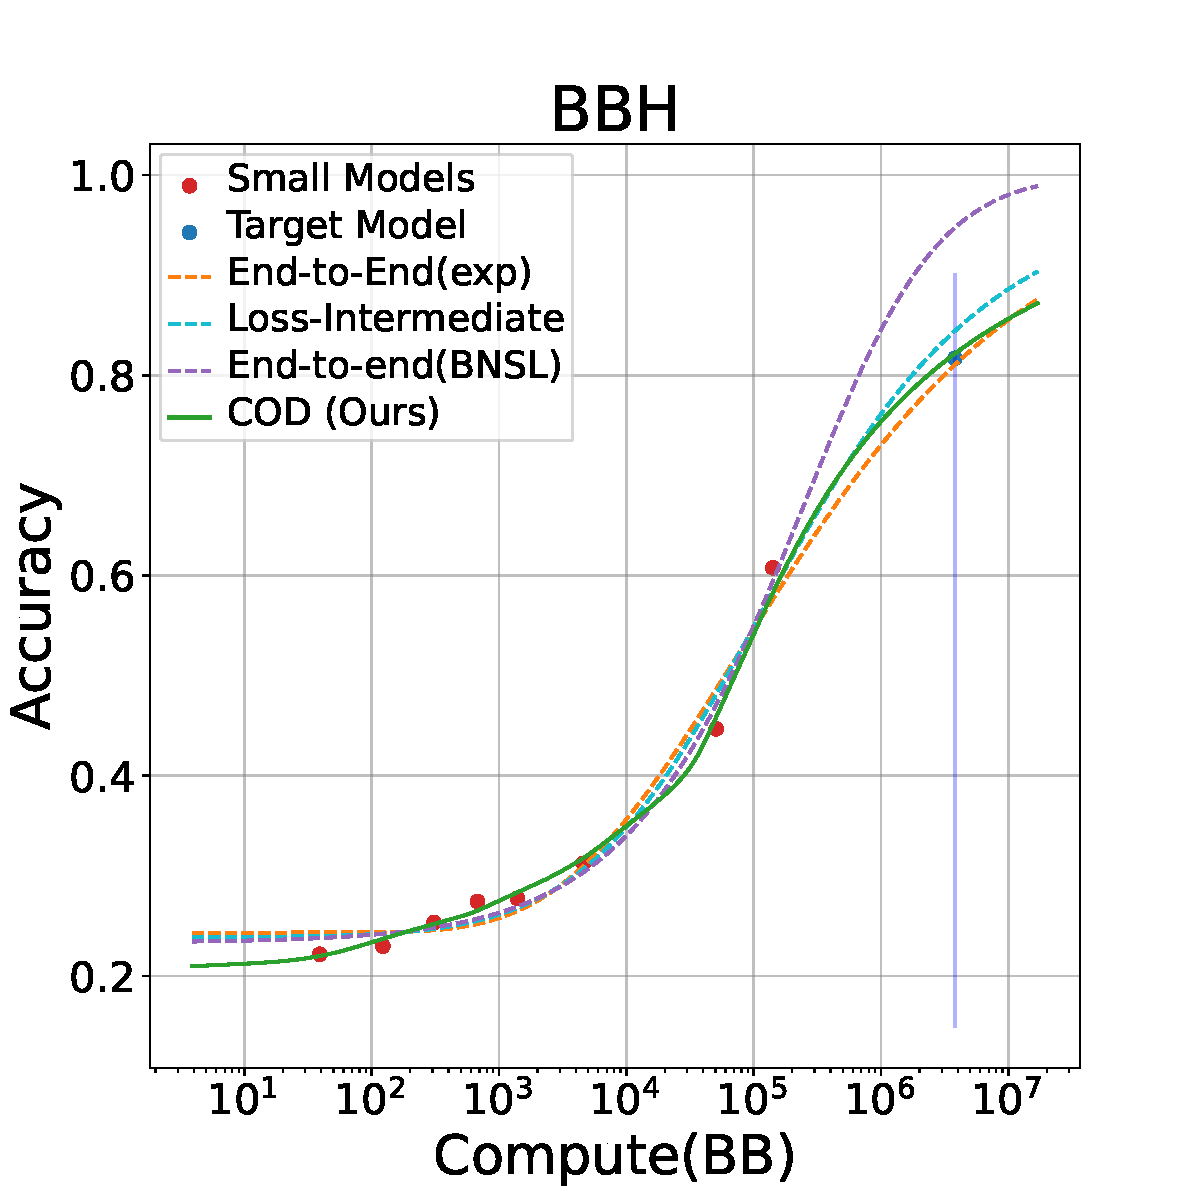
\includegraphics[width=\textwidth]{figures/experiments/perf_compute/BBH.pdf}
    \end{minipage}
    \begin{minipage}{0.24\textwidth}
        \centering
        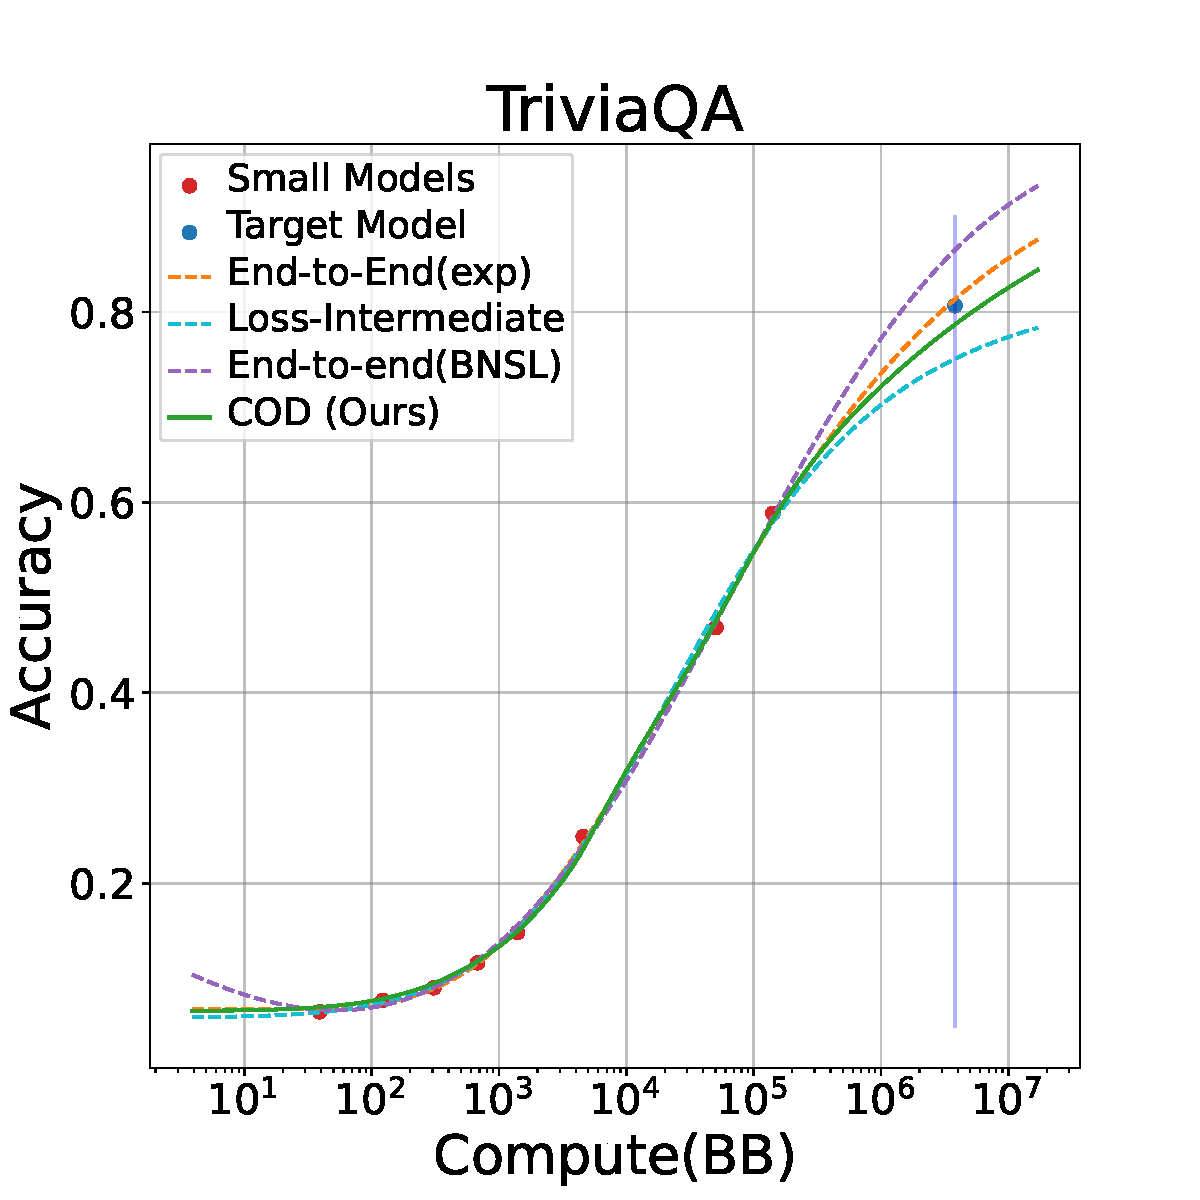
\includegraphics[width=\textwidth]{figures/experiments/perf_compute/TRIVIAQA.pdf}
    \end{minipage}

    \begin{minipage}{0.24\textwidth}
        \centering
        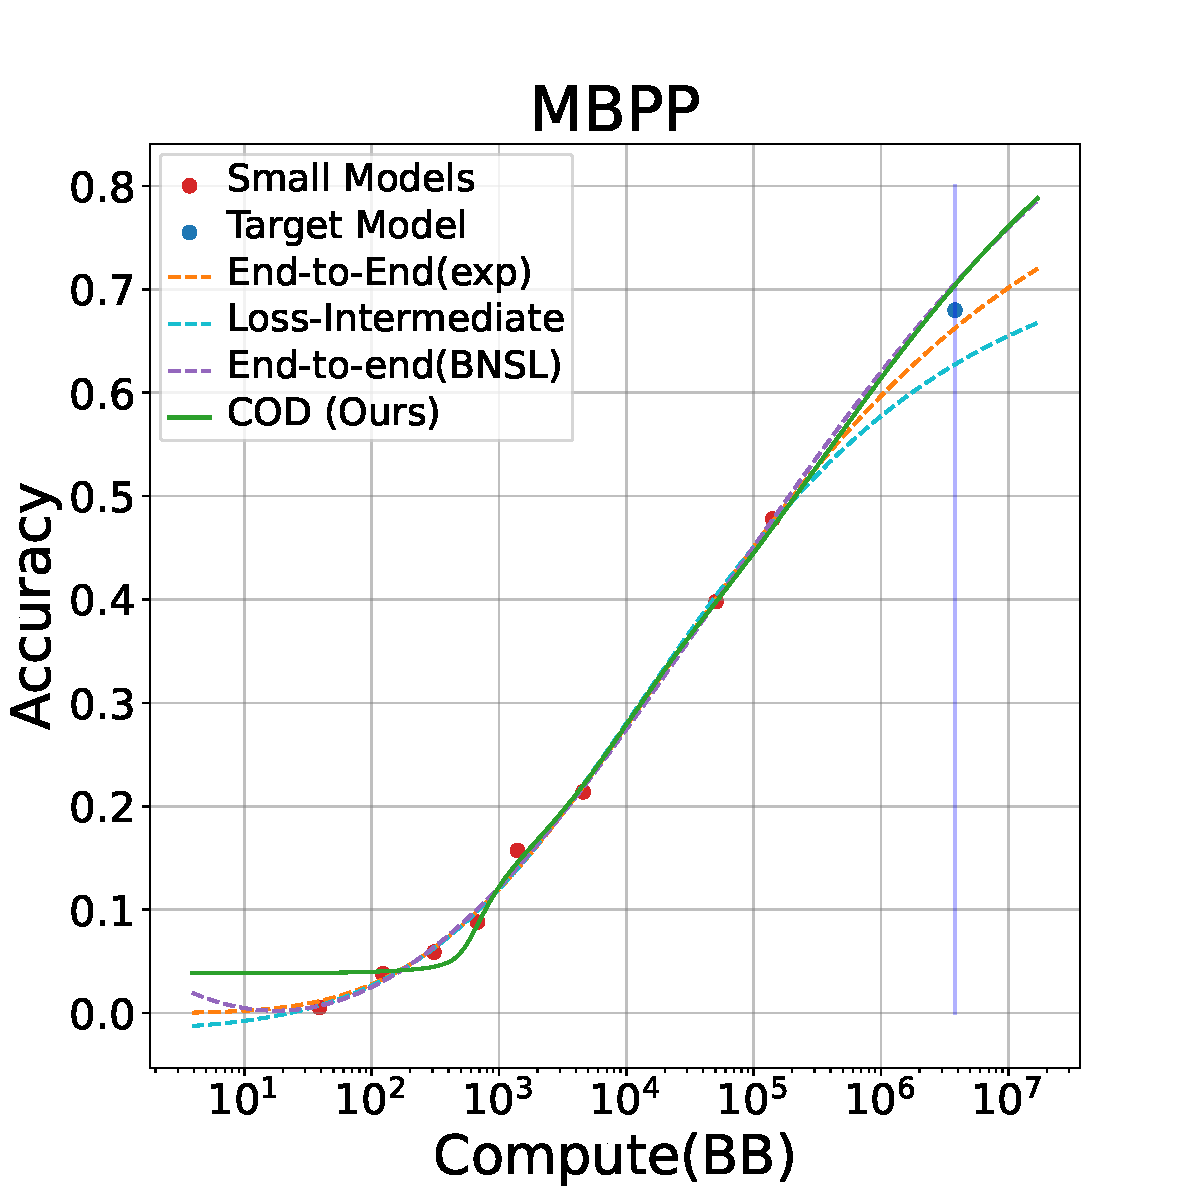
\includegraphics[width=\textwidth]{figures/experiments/perf_compute/MBPP.pdf}  % 替换为实际文件名
    \end{minipage}
    \begin{minipage}{0.24\textwidth}
        \centering
        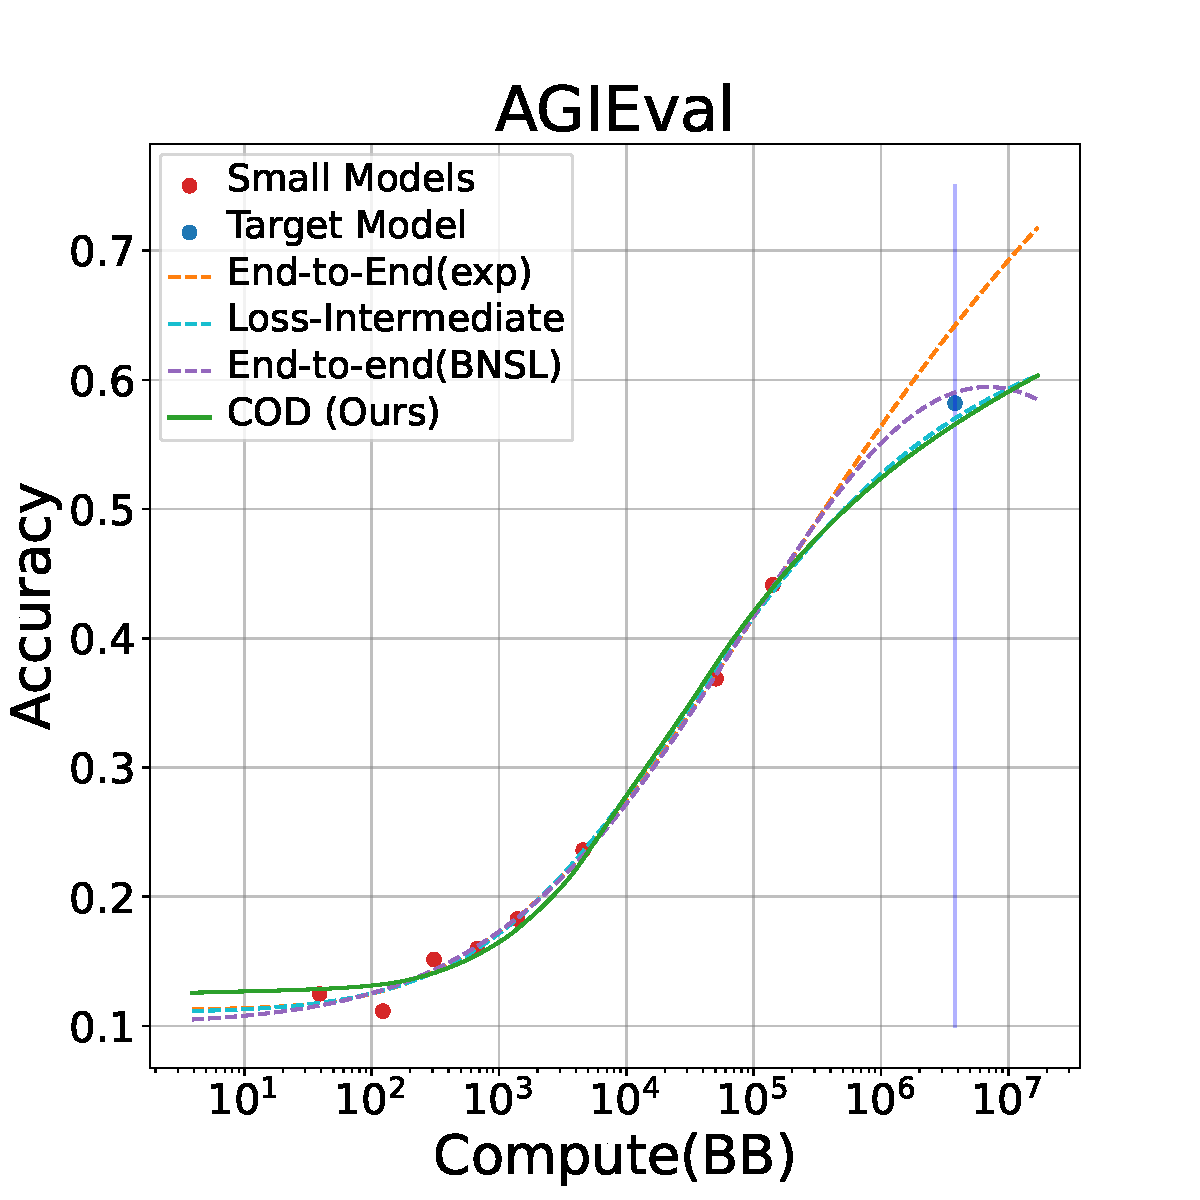
\includegraphics[width=\textwidth]{figures/experiments/perf_compute/AGIEVAL.pdf}  % 替换为实际文件名
    \end{minipage}
    \begin{minipage}{0.24\textwidth}
        \centering
        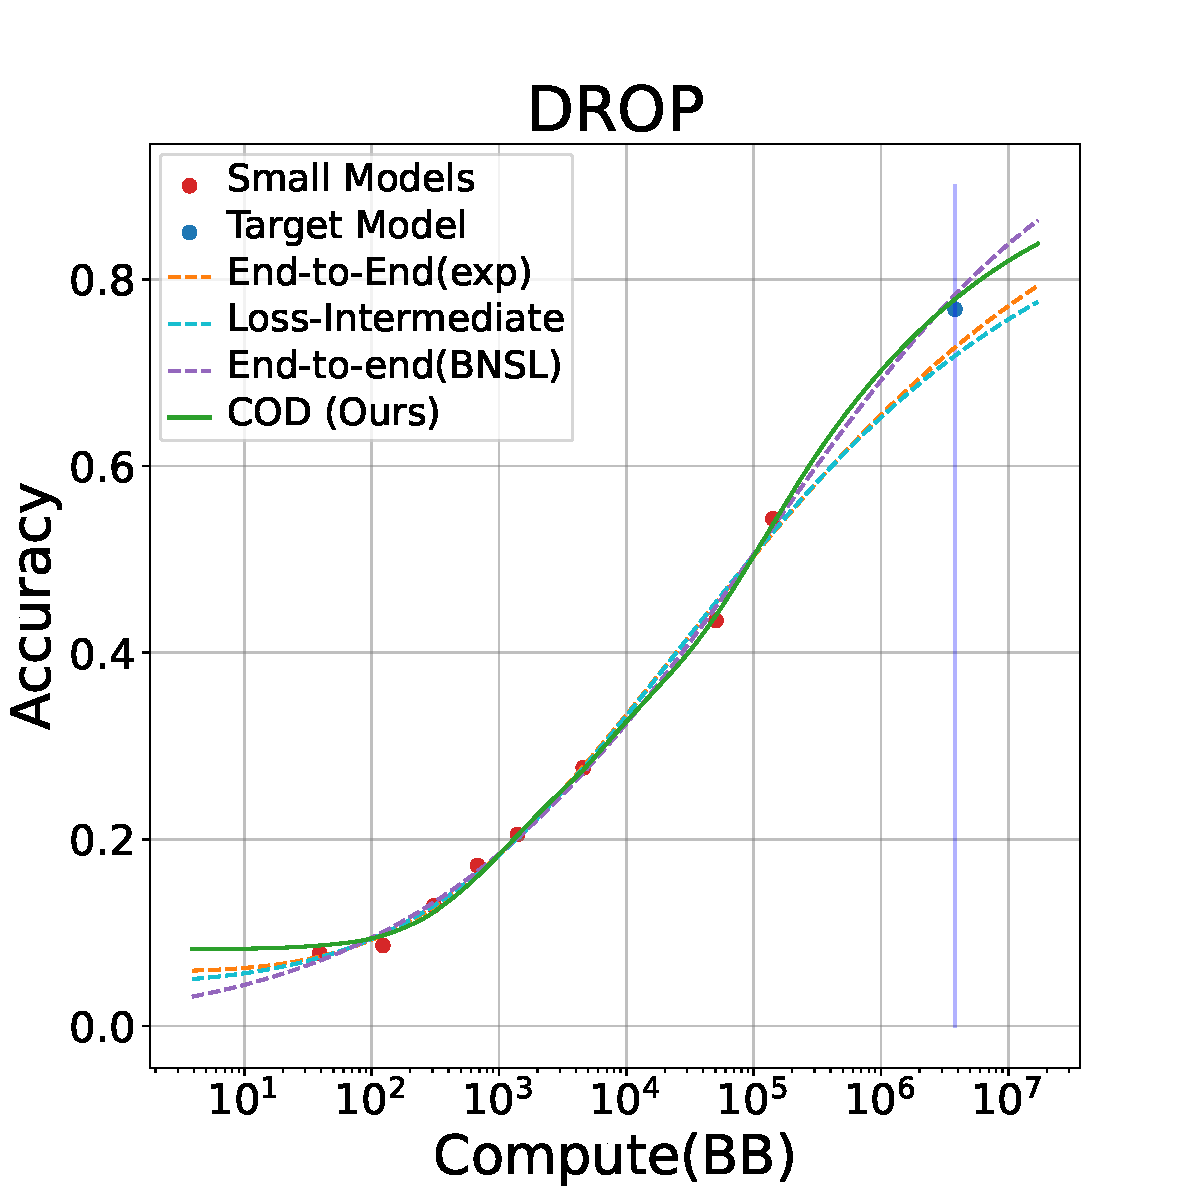
\includegraphics[width=\textwidth]{figures/experiments/perf_compute/DROP.pdf}  % 替换为实际文件名
    \end{minipage}
    \begin{minipage}{0.24\textwidth}
        \centering
        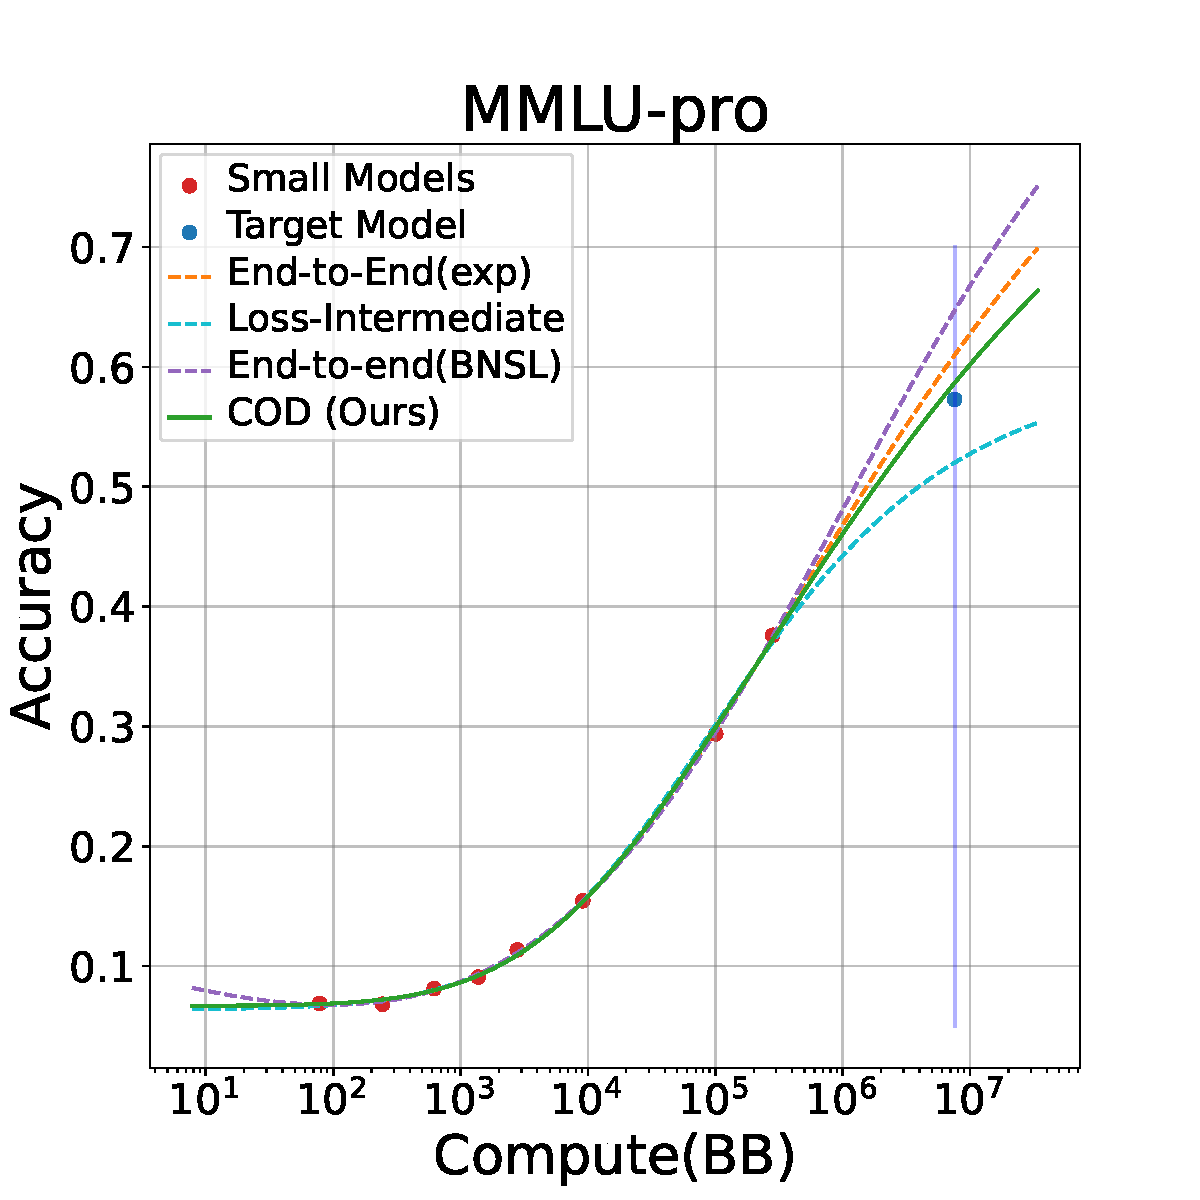
\includegraphics[width=\textwidth]{figures/experiments/perf_compute/MMLU-pro.pdf}  % 替换为实际文件名
    \end{minipage}
    \caption{Performance-compute relationship for different prediction methods on eight evaluation sets.}
    \label{fig:prediction_experiment_vis}
    % \vspace{-5pt}
\vspace{-10pt}

\end{figure}

\cref{fig:prediction_experiment_vis} visualizes the performance-compute relationships. The COD method does not merely extend the existing scaling trend; instead, it effectively predicts whether growth slowdown will occur subsequently and enables better estimation of the magnitude of curve bending.
On the BBH dataset, while End-to-end(exp) and loss-intermediate approaches perform comparably to COD, they show poor fitting on small-model data. COD reveals a more complex, better-fitted multi-phase trajectory. On MATH and MMLU-pro, where predicting accelerated growth versus plateaus is crucial, the loss-intermediate method underestimates model ceilings, and two end-to-end methods exceeds 3\% error. COD's superior performance stems from its nuanced analysis of difficulty distributions and scaling laws, allowing it to predict growth in challenging sets and capture diminishing returns in saturated sets.

\vspace{-5pt}
\subsection{Ablation Study}
To further validate the generalizability of the COD method, we conduct ablation experiments on \camera{different architecture}, clustering method and extrapolation function, while in the Appendix~\ref{sec:additional_ablation} we discuss ablation studies on the selection criteria for predictable subsets, interpolation mapping methods, and the influence of anchor point on predictions. We also examine its predictive capabilities after continual training with results documented in Appendix~\ref{sec:ppct}.

% \revise{\subsubsection{Prediction for a Medium-size Model}
% \label{sec:medium}
% The COD method is also effective for predicting the capabilities of medium-size language models. To demonstrate this, we conducted an experiment to predict the performance of a 12B model using source models ranging from 122M to 1.9B parameters. This setup maintains a similar ~6$\times$ parameter-size ratio as our main experiment (predicting 70B from models up to 12B).

% For this experiment, clustering relied exclusively on the passrate@100 data from the 122M to 1.9B source models to prevent data leakage from the target model. The results in~\cref{tab:12B_results} show that COD is more robust and less demanding on the size of source models compared to the baselines. For instance, the baseline methods perform poorly on the BBH benchmark, In contrast, COD accurately captures the trend of accuracy growth as compute increases and yields precise extrapolations. We will include a plot of this curve in the main text to visually demonstrate the clear advantage of COD.

% The prediction errors of all methods for the 12B model are significantly higher than those for the 70B model reported in~\cref{subsec:Prediction_Experiments}. Extrapolation accuracy improves when larger source models are employed for fitting, as a greater number of samples have ``emerged''. If the largest source model is excessively small, numerous samples remain ``unemerged'', resulting in substantial errors when extrapolating to a significantly larger model.}

% \begin{table*}[!t]
% \small
% \setlength{\tabcolsep}{1.8pt} % 保持原列间距设置
% \centering
% \caption{Absolute prediction error (\%) on evaluation sets for predicting the performance of the 12B model. Errors < 2\% are considered accurate (green), while errors > 5\% are considered invalid (red). $\downarrow$ indicates lower is better.}
% \begin{tabular}{c|c|cc|cc|cc|cc} % 列结构：任务/指标 | 真值 | 4组[Prediction|Error]
% \toprule
% \multirow{2}{*}{Task Sets/Metrics} & \multirow{2}{*}{Ground Truth} & \multicolumn{2}{c|}{\textbf{Loss-intermediate}} & \multicolumn{2}{c|}{\textbf{End-to-end}} & \multicolumn{2}{c|}{\textbf{BNSL}} & \multicolumn{2}{c}{\textbf{COD}} \\
% \cmidrule(lr){3-10} % 分隔线覆盖所有方法的Prediction-Error列
% & & Prediction & Error & Prediction & Error & Prediction & Error & Prediction & Error \\
% \toprule
% \multicolumn{10}{c}{\textbf{Overall Metrics}} \\ % 横向标题适配10列
% \midrule
% Mean & - & - & 14.92 & - & 10.52 & - & 17.42 & - & \textbf{4.68} \\
% Max & - & - & 23.82 & - & 24.43 & - & 28.26 & - & \textbf{10.39} \\
% \midrule
% \multicolumn{10}{c}{\textbf{Individual Task Sets}} \\ % 横向标题适配10列
% \midrule
% GSM8k & 70.47 & 60.86 & \redhl{9.61} & 63.66 & \redhl{6.81} & 80.99 & \redhl{10.52} & 60.08 & \redhl{10.39} \\
% MATH & 30.85 & 41.53 & \redhl{10.68} & 34.36 & 3.51 & 49.26 & \redhl{18.41} & 28.48 & 2.37 \\
% BBH & 60.76 & 36.94 & \redhl{23.82} & 36.33 & \redhl{24.43} & 36.10 & \redhl{24.66} & 57.751 & 3.05 \\
% TriviaQA & 58.84 & 68.42 & \redhl{9.57} & 59.88 & \greenhl{1.04} & 87.10 & \redhl{28.26} & 57.92 & \greenhl{0.93} \\
% MBPP & 47.80 & 28.53 & \redhl{19.27} & 36.51 & \redhl{11.29} & 27.95 & \redhl{19.85} & 44.50 & 3.30 \\
% AGIEval & 44.13 & 33.91 & \redhl{10.22} & 35.40 & \redhl{8.74} & 34.12 & \redhl{10.01} & 47.53 & 3.40 \\
% DROP & 54.35 & 35.05 & \redhl{19.30} & 37.19 & \redhl{17.16} & 36.73 & \redhl{17.62} & 63.50 & \redhl{9.14} \\
% MMLU-pro & 37.60 & 20.74 & \redhl{16.86} & 26.41 & \redhl{11.20} & 27.59 & \redhl{10.01} & 42.42 & 4.82 \\
% \bottomrule
% \end{tabular}
% \label{tab:12B_results}
% % \vspace{-10pt}
% \end{table*}

\subsubsection{\camera{Prediction on MoE models}}
% COD方法依赖于样本粒度的重复评测以及聚类，带来了额外的复杂度与算力开销。然而难度特征是属于题目本身与模型相对独立，聚类结果应该可以在不同模型族的预测任务中进行服用。我们下面验证利用Dense小模型获得预测结果可以外推到一系列MoE模型上。
% \camera{The COD approach relies on repeated sample-level evaluation and clustering, which introduces additional complexity and computational overhead. However, difficulty characteristics are inherent to the tasks themselves and are relatively model-agnostic, so the clustering results should be reusable across prediction tasks of different model families. Below, we verify that prediction results derived from small dense models can be extrapolated to a range of MoE models.
% To verify the robustness of the clustering results, we perform one-shot evaluation across benchmarks on a 32B activated-parameter MoE model, using the clustering results obtained from pre-trained dense models. Comparative results are shown in \cref{tab:MoE_exp}.}
% 可以看出在夸模型结构的预测上，COD方法取得了最优的平均预测误差，说明其难度特征与类簇在不同模型族之间具有一定迁移效果。但预测精度相比预测Dense模型有所下降，估计难度特征的模型与用于预测外推的模型保持一致可以最小化类内任务的Scaling差异，并取得更好的预估结果。
% \camera{It can be seen that the COD method achieves the best average prediction error in cross-architecture prediction, indicating that its difficulty characteristics and clusters have a certain transferability across different model families.
% However, the prediction accuracy decreases compared with forecasting on dense models.
% We conjecture that keeping the model used for estimating difficulty characteristics consistent with the model for extrapolation can minimize the scaling differences of within-cluster tasks and yield better estimation results.}

\camera{
COD relies on repeated sample-level evaluation and clustering, introducing additional computational overhead. 
However, difficulty characteristics are task-inherent and largely model-agnostic, suggesting that the resulting clusters can generalize across model families. 

To test this transferability, we conduct one-shot evaluations on a 32B activated-parameter MoE model using clusters derived from pre-trained dense models. Results in \cref{tab:MoE_exp} show that COD achieves the lowest average prediction error in cross-architecture extrapolation, indicating that its difficulty features and clusters transfer effectively across model families. 
Nevertheless, prediction accuracy is lower than in dense-to-dense extrapolation. We hypothesize that aligning the model used for difficulty estimation with the target model for extrapolation reduces intra-cluster scaling discrepancies and improves prediction accuracy.
}
\begin{table*}[!t]
\small
\setlength{\tabcolsep}{1.8pt} % Keep this if column spacing is critical
\centering
\caption{Absolute prediction error (\%) on evaluation sets for predicting the performance of the 32B MoE model. Errors < 2\% are considered accurate (green), while errors > 5\% are considered invalid (red). $\downarrow$ indicates lower is better.}
\begin{tabular}{c|cc|ccccccc}
\toprule
\multirow{2}{*}{Method} & \multicolumn{2}{c|}{Overall Metrics} & \multicolumn{7}{c}{Individual Task Sets} \\
\cmidrule(lr){2-3} \cmidrule(lr){4-10}
& Mean$\downarrow$ & Max$\downarrow$ & GSM8k & MATH & BBH & TriviaQA & MBPP & AGIEval & DROP \\
\midrule
Loss-intermediate & 3.65 & \textbf{7.24} & \greenhl{0.45} & \greenhl{0.62} & 4.48 & \greenhl{0.36} & 4.92 & \redhl{7.24} & 4.55 \\
End-to-end(exp) & 3.95 & 7.86 & 2.75 & \greenhl{1.43} & 3.88 & \greenhl{1.72} & \redhl{7.86} & \redhl{7.79} & 2.21 \\
% End-to-end(BNSL) &  &  &  &  &  &  &  &  &  \\
\midrule
COD (Complete) & \textbf{3.11} & 8.11 & \greenhl{0.54} & \greenhl{1.72} & \redhl{5.29} & \greenhl{0.27} & \redhl{8.11} & \greenhl{0.57} & \redhl{5.24} \\
\bottomrule
\end{tabular}
\label{tab:MoE_exp}
\vspace{-8pt}
\end{table*}

\subsubsection{Comparison of Clustering Methods}
\label{sec:clustering_ablation}

We assess the impact of different clustering algorithms on prediction accuracy. The goal is to achieve tight intra-cluster difficulty similarity (low average distance to center) while maintaining cluster stability (min. 10 samples/cluster). We compare our Improved-MeanShift with DBScan, MeanShift, and K-Means. For K-Means, we adjust it to approximate our goals: (1) search for $k$ yielding min. cluster sizes $\approx 10$; (2) treat samples outside a radius (e.g., 2$\times$ average intra-cluster distance) from any cluster center as outliers, and we ensure clusters don't drop below 10 samples. We term this "Improved-KMeans" for this comparison. Clustering quality is measured by Intra-cluster Average Distance (IAD) and Outlier Rate (OR). Prediction benefits are measured by Extrapolation Error (EE) on the predictable subset and Final prediction Error (FE) on the full evalset. (\cref{tab:clustering_prederror}).

\begin{table*}[!t]
\centering
\scriptsize % 使用更小的字体 (比 footnotesize 更小)
\caption{Clustering performance across different algorithms on metrics including IAD (Intra-cluster Average Distance$\downarrow$), OR (Outlier Rate \%), EE (Extrapolation Error$\downarrow$), FE (Final Prediction Error$\downarrow$). The bottom lines show the mean and max EE and FE across evalsets.}
\setlength{\tabcolsep}{1.5pt} % 进一步减小列间距
\resizebox{\textwidth}{!}{% 自适应页面宽度
\begin{tabular}{l|cccc|cccc|cccc|cccc|cccc}
\toprule
\multirow{2}{*}{Dataset} & \multicolumn{4}{c|}{KMeans} & \multicolumn{4}{c|}{DBScan} & \multicolumn{4}{c|}{MeanShift} & \multicolumn{4}{c|}{Improved-KMeans} & \multicolumn{4}{c}{Improved-MeanShift} \\
\cmidrule(lr){2-5} \cmidrule(lr){6-9} \cmidrule(lr){10-13} \cmidrule(lr){14-17} \cmidrule(lr){18-21}
& IAD & OR & \textbf{EE} & \textbf{FE} & IAD & OR & \textbf{EE} & \textbf{FE} & IAD & OR & \textbf{EE} & \textbf{FE} & IAD & OR & \textbf{EE} & \textbf{FE} & IAD & OR & \textbf{EE} & \textbf{FE} \\
\midrule

GSM8k    & 0.22 & - & \textbf{0.01} & \textbf{0.00} & 0.51 & 0.53 & 4.08 & 4.12 & 0.29 & 0.61 & 0.67 & 0.74 & \textbf{0.13} & 2.73 & 3.92 & 4.08 & 0.16 & 7.05 & 0.31 & 2.68 \\
MATH     & 0.22 & - & 2.62 & 2.34 & 0.48 & 0.68 & 4.38 & 4.16 & 0.21 & 1.44 & 2.55 & 2.26 & \textbf{0.09} & 2.22 & \textbf{0.81} & \textbf{0.51} & 0.11 & 6.26 & 0.84 & 0.79 \\
BBH      & 0.63 & - & 8.16 & 8.99 & 0.71 & 18.92 & 3.53 & 4.36 & 0.27 & 20.72 & 2.12 & 0.65 & \textbf{0.20} & 37.23 & \textbf{0.02} & 2.17 & 0.21 & 33.58 & 0.54 & \textbf{0.47} \\
TriviaQA & 0.44 & - & 2.97 & 2.46 & 0.70 & 6.38 & \textbf{1.11} & \textbf{0.81} & 0.25 & 6.77 & 3.64 & 4.90 & \textbf{0.12} & 11.97 & 1.18 & 1.12 & 0.19 & 11.54 & 1.56 & 1.97 \\
MBPP     & 0.34 & - & 2.53 & 2.67 & 0.51 & 12.80 & \textbf{1.57} & 1.41 & 0.22 & 15.60 & 2.40 & \textbf{1.22} & \textbf{0.17} & 19.40 & 2.39 & 3.25 & \textbf{0.17} & 21.60 & 1.61 & 2.42 \\
AGIEval  & 0.46 & - & 2.61 & 2.68 & 0.56 & 3.67 & 6.43 & 6.27 & 0.29 & 2.99 & 2.63 & 3.23 & \textbf{0.15} & 7.60 & 5.96 & 5.56 & 0.21 & 11.50 & \textbf{1.11} & \textbf{1.64} \\
DROP     & 0.56 & - & 1.66 & 1.64 & 0.67 & 11.08 & 3.03 & 2.66 & 0.25 & 11.81 & 4.18 & 4.00 & \textbf{0.14} & 21.42 & 3.99 & 5.24 & 0.20 & 19.88 & \textbf{1.44} & \textbf{1.05} \\
MMLU-pro & 0.32 & - & 3.69 & 3.69 & 0.42 & 0.56 & 3.72 & 3.69 & 0.29 & 0.39 & 3.15 & 3.08 & \textbf{0.16} & 2.85 & \textbf{0.56} & \textbf{0.61} & 0.22 & 4.40 & 1.26 & 1.39 \\
\midrule
\textbf{Mean} & - & - & 3.03 & 3.06 & - & - & 3.48 & 6.43 & - & - & 2.67 & 2.51 & - & - & 2.35 & 2.82 & - & - & \textbf{1.08} & \textbf{1.55} \\
\textbf{Max}  & - & - & 8.16 & 8.99 & - & - & 4.38 & 4.36 & - & - & 4.18 & 4.90 & - & - & 5.96 & 5.56 & - & - & \textbf{1.61} & \textbf{2.68} \\
\bottomrule
\end{tabular}
} % 结束 resizebox
\label{tab:clustering_prederror}
\vspace{-5pt}
\end{table*}


\cref{tab:clustering_prederror} shows Improved-KMeans and Improved-MeanShift yield better clustering (lower IAD) due to their intra-cluster distance constraints. The results also confirm these methods lead to lower EE and FE. Although Improved-KMeans has the best IAD,  it performs poorly on GSM8k, AGIEval, and DROP. This is likely because K-Means requires pre-specifying $k$, and our search for $k$ can be unstable, leading to large errors on some sets. In contrast, our Improved-MeanShift, which automatically determines $k$ based on distance constraints, offers more stable clustering and the lowest maximum prediction error.

\subsubsection{Different Extrapolation Formulas}
\label{sec:ablation_extrapolation}
\begin{table*}[!t]
\centering
\small
\caption{Ablation study on extrapolation formulas. EE, TR, FE shown for BBH, MATH, MMLU-pro.}
\begin{tabular}{c|ccc|ccc|ccc}
\toprule
\multirow{2}{*}{Method} & \multicolumn{3}{c}{BBH} & \multicolumn{3}{c}{MATH} & \multicolumn{3}{c}{MMLU-pro} \\
\cmidrule(lr){2-4} \cmidrule(lr){5-7} \cmidrule(lr){8-10}
& EE$\downarrow$ & TR(\%) & FE$\downarrow$ & EE$\downarrow$ & TR(\%) & FE$\downarrow$ & EE$\downarrow$ & TR(\%) & FE$\downarrow$ \\
\midrule
w/o Random Guess ($f_1$) & 10.40 & 48.29 & 11.65 & 3.96 & 76.82 & 3.22 & 4.40 & 95.05 & 4.32 \\
w/o Constant c ($f_2$) & 2.15 & 57.21 & 4.10 & 1.50 & 76.82 & 1.36 & 3.85 & 95.60 & 3.96 \\
Direct Power Law ($f_3$) & 8.90 & 49.05 & 8.85 & 3.33 & 76.82 & 2.70 & 4.30 & 95.15 & 4.20 \\
Ours ($f$) & \textbf{0.54} & 53.39 & \textbf{0.47} & \textbf{0.84} & 76.82 & \textbf{0.79} & \textbf{1.26} & 94.38 & \textbf{1.39} \\
\bottomrule
\end{tabular}
\label{tab:ablation_results}
\vspace{-5pt}
\end{table*}
We ablate our proposed fitting formula $f(C)=g+(1-g) \cdot e^{-aC^{-b}-c}$ (Ours) by removing or modifying components:
(1) $f_1(C)=e^{-aC^{-b}-c}$ (w/o random guess);
(2) $f_2(C)=g+(1-g) \cdot e^{-aC^{-b}}$ (w/o constant $c$);
(3) $f_3(C) = e^{-aC^{-b}}$ (Direct Power Law~\citep{hu2023predicting}).
\cref{tab:ablation_results} shows Extrapolation Error (EE), Task Ratio of predictable subset (TR), and Final prediction Error (FE).
Our proposed formula $f$ consistently achieves the lowest EE and FE. $f_1$ struggles with finite-answer tasks where small models have non-zero scores. $f_2$ inaccurately assumes perfect scores are attainable, ignoring data limitations and task ambiguities. The direct power law ($f_3$) fails to model the 0-1 metric range and the varying difficulty of improvement near random guess and saturation. \camera{The weak correlation between TR and prediction error demonstrates the robustness of our COD framework: even when the proportion of the predictable subset is low due to non-emergent tasks, the performance of non-extrapolatable tasks can still be accurately inferred through the proposed mapping function.}
% TR's minor influence on prediction error suggests robustness; even with low TR due to non-emergent tasks, their performance can be largely predicted via mapping.



\vspace{-5pt}
\section{Conclusion and Discussion}
\vspace{-7pt}
\label{sec:discussion}
% In this work, we introduce a novel downstream performance scaling framework including (1) the COD method that effectively models the underlying diverse scaling patterns of evaluation tasks
\camera{In this work, we propose a novel framework for predicting LLM downstream performance scaling, which consists of three key contributions: (1) the COD framework that effectively models the intrinsic diverse scaling patterns of tasks in the evaluation set}; (2) a scaling law for downstream task performance that provides a fitting formula for performance-compute extrapolation; and (3) a systematic methodology for identifying and leveraging predictable subset that provides a robust intermediate metric for accurate full-set performance predictions.
We discuss the limitations and future works in Appendix~\ref{sec:limiations}.
% Looking forward, our approach can be further expanded across model architectures, training methods, and evaluation set types, while extending this framework to address chain-of-thought reasoning patterns offer promising avenues for future research.

% \paragraph{Boarder Impact} 
% \section{Boarder Impact}
% The LLMs performance scaling prediction method proposed in this work can be used to guide decision-making for training LLMs and to monitor whether the LLM training process aligns with expectations. Accurate prediction allows for better planning of compute and human resources, thereby playing a valuable role in scientifically advancing the training of larger LLMs. However, if the prediction results are inaccurate, it may lead to outcomes that do not meet expectations for the invested resources, potentially resulting in resource waste or economic losses.

\section*{Ethics Statement}
\label{sec:social_impact}
We have read and adhered to the ICLR Code of Ethics. This work proposes a computational framework to enable more efficient resource allocation in the training of LLMs. The research is methodological in nature and aims to support more sustainable and responsible practices within the field of AI development.

We provide a detailed account of our methods, theoretical proofs, and experimental settings. We openly discuss the limitations of our framework in Appendix~\ref{sec:limiations}. This study does not involve human subjects or the use of sensitive personal data.

We utilized language models at the writing level, including checking for grammatical errors in the article and modifying expressions. The use of language models had no impact on the article's innovative contributions, experiments, or analytical perspectives.



\section*{Reproducibility Statement}
We have made extensive efforts to ensure the reproducibility of our work. The core methodology, the Clustering-On-Difficulty (COD) framework, is detailed in \cref{sec:method}. The improved MeanShift clustering algorithm is described in \cref{sec:method-clustering} , with full pseudocode provided in Appendix~\ref{sec:improved} (Algorithm 1). Our performance scaling law (Theorem 1) is presented in \cref{sec:fitting} , with a complete proof available in \cref{sec:prop_proof}. We discuss the additional computational cost of the COD method in Appendix~\ref{append:compute}.

Our experimental setup, including model architectures, training data philosophy, and hyperparameters, is thoroughly documented in \cref{sec:exp_setups} and Appendix~\ref{append:setting} , with specific model configurations listed in \cref{tab:model_configs_dense}. The evaluation benchmarks, protocols, and few-shot settings are described in \cref{sec:exp_setups} and summarized in \cref{tab:evaluation_info}. Extensive ablation studies validating our component choices—including extrapolation formulas (\cref{sec:ablation_extrapolation}), clustering algorithms (Appendix~\ref{sec:clustering_ablation}), interpolation methods (Appendix~\ref{sec:interpolation_ablation}), and criteria for filtering clusters (Appendix~\ref{sec:criteria})—are provided to support our findings. We visualize the task difficulty distribution for each evalset in Appendix~\ref{sec:difficulty_distribution}.

\bibliographystyle{plainnat}
\bibliography{main}
% }

% \clearpage

\newpage

% \appendix

\appendix

{\small\tableofcontents}  % 现在只显示 appendix

% \tableofcontents
\setcounter{table}{0} 
\setcounter{figure}{0}
\setcounter{proposition}{0}
\setcounter{theorem}{0}

\renewcommand{\thefigure}{A\arabic{figure}}
\renewcommand{\thetable}{A\arabic{table}}
\renewcommand{\thetheorem}{A\arabic{theorem}}



% \renewcommand{\thefigure}{A\arabic{figure}}
% \renewcommand{\thetable}{A\arabic{table}}
% \renewcommand{\theproposition}{A.\arabic{proposition}}
% \renewcommand{\thesection}{Appendix \Alph{section}}
% \crefname{section}{Appendix}{Appendices}
% \Crefname{section}{Appendix}{Appendices}

\section{Improvements of Clustering Algorithm}
\label{sec:clustering_opt}
% 具体来说，我们迭代式地使用MeanShift算法，并预设一个聚类半径R，以及一个类簇的最小样本数量K。在每次迭代中，对于完成聚类的样本，我们检验每个样本到类簇中心的距离是否大于R，并把大于R的样本重新标记为没有聚类。同时，对于样本数量小于K的聚类，我们也把这些类的样本标记为没有聚类。在每次迭代结束，我们把MeanShift的离群点与我们标记出没有聚类的样本重新纳入下一轮地聚类中，直到所有样本类别不再发生变化。我们把我们把伪代码展示在\cref{improved_shift}。
\subsection{Improved MeanShift Algorithm}
\label{sec:improved}
We iteratively apply the MeanShift algorithm with an \camera{adaptive} cluster radius $R$ and a minimum cluster size $K$. 
In each iteration, for the clustered samples, we examine whether the distance between each sample and its cluster center exceeds R, and relabel those samples that exceed this threshold as unclustered. 
For clusters containing fewer than K samples, we mark all samples in these clusters as unclustered. 
At the end of each iteration, we incorporate both the outliers from MeanShift and our marked unclustered samples into the next round of clustering, continuing this process until no further changes occur in sample labels. We present the pseudocode in \cref{algo:improved_meanshift}.

\begin{algorithm}
\caption{Iterative MeanShift Clustering Algorithm}
\label{algo:improved_meanshift}
\begin{algorithmic}[1]
\State \camera{Calculate adaptive radius: $R=\min(\mathrm{estimate\_bandwidth}(Q),U)$}
\State Initialize all labels in the evaluation set to $-1$
\Repeat
    \State Perform MeanShift clustering with radius $R$ on all samples labeled $-1$
    \State Assign new labels to clustered samples
    \For{each newly labeled sample $i$}
        \State Calculate distance $\mathrm{dist}_i$ to its cluster center
        \If{$\mathrm{dist}_i > R$}
            \State Reset label to $-1$
        \EndIf
    \EndFor
    \For{each cluster}
        \If{number of samples in cluster $< K$}
            \State Reset all samples in this cluster to $-1$
        \EndIf
    \EndFor
    \State Renumber all non-$\{-1\}$ newly labeled samples to avoid overlap with old labels
\Until{no label changes}
\end{algorithmic}
\end{algorithm}

In the experiment, $K$ is empirically set to $10$, which has been verified through extensive experiments to be a reasonable and robust value. \camera{To determine the clustering radius $R$, we employ the \textit{estimate\_bandwidth} function from the \textit{sklearn.cluster} library. This utility automatically computes a bandwidth value that balances clustering granularity and stability based on the underlying distribution of the data. The function is governed by a quantile hyperparameter $Q$, which typically ranges from $0.1$ to $0.5$. Given our framework's stringent requirements for minimizing intra-cluster variance, we adopt a conservative value of $Q=0.1$ in practice. Furthermore, considering that sample sizes and difficulty distributions vary significantly across different evaluation sets, the automatically estimated bandwidth may occasionally become excessively large. To mitigate this risk, we introduce a global upper bound $U$ on the bandwidth. Specifically, we define $U = max\_distance/10$, where $\text{max\_distance}$ represents the theoretical maximum distance between any two vectors in the difficulty feature space and $10$ is a empirical constant. In our experimental setup, the feature vectors are 9-dimensional with each element inherently bounded within the range $[0, 1]$. Consequently, the maximum possible Euclidean distance is calculated as $\sqrt{1^2 \times 9} = 3$, yielding an upper bound of $U = 0.3$.}

% The fixed radius $R$ depends only on the value range and dimensionality (i.e., the number of predictive models) of the difficulty feature vectors. In our experiments, we fixed $R=0.3$ for all evaluation sets to ensure consistent overall clustering performance. 

% For experiments with different numbers of small models used for fitting, the value of $R$ needs to be adaptively adjusted due to changes in the dimensionality of the feature vector. For instance, in the experiment of predicting the 12B-parameter model, $R$ was empirically reduced from $0.3$ to $0.2$ to ensure that the intra-class error is reasonable.


\paragraph{Filtering zero-performance samples.}
In the evaluation set, there may exist a few extremely difficult problems that require sufficient model parameters to emerge. All small models may fail to solve these problems even after 100 evaluation attempts, resulting in difficulty feature vectors of all zeros. We refer to these as zero-performance samples. Their presence leads to two issues:
\begin{enumerate}[leftmargin=1.5em]
    \item Zero performance on small models does not necessarily indicate zero accuracy on large models. For these samples, we cannot estimate when emergence will occur or predict large model metrics.
    \item During clustering, they may be confused with other low-performing but non-zero samples. Including them in the same cluster would lower the expected accuracy of that cluster, leading to inaccurate fitting and extrapolation later.
\end{enumerate}

Therefore, we pre-filter these zero-performance samples before clustering, treating them as outliers that do not participate in the clustering process. 
% This approach eliminates the need to consider their metrics under large models during subsequent extrapolation and prevents disruption to the clustering of the remaining samples.
This approach obviates the necessity of considering their metrics under large models during subsequent extrapolation, and prevents disruption to the clustering of the remaining samples.



\subsection{Smoothing Techniques}
\label{sec:smoothing}
% \noindent\textbf{Horizontal smoothing: adjacent checkpoint smoothing.}
Metric fluctuations of individual samples in downstream tasks are not solely due to limited sampling. Another potential factor is noise from uneven data distribution in recent training batches. Therefore, in addition to performing 100 evaluations to mitigate sampling variance, we evaluated 100 times on each of the adjacent checkpoints before and after the selected model. We then averaged these accuracy expectation values across three checkpoints, further reducing sampling variance while offsetting noise from uneven training data distribution. This approach also reduces the number of zero-performance samples, further improving clustering and prediction effectiveness.






\section{Proof of Theorem 1}
\label{sec:prop_proof}
We use \cref{proof:am_gm} to derive the scaling law for downstream task performance (\cref{main:proof:task_scaling_law}).
\begin{lemma}[Arithmetic-geometric mean difference]
\label{proof:am_gm}
For any sequence of positive real numbers $\{x_i\}_{i=1}^n$, let:
\begin{itemize}
    \item $\mu_a = \frac{1}{n}\sum_{i=1}^n x_i$ be the arithmetic mean;
    \item $\mu_g = \prod_{i=1}^n x_i^{1/n}$ be the geometric mean; 
    \item $\sigma^2 = \frac{1}{n}\sum_{i=1}^n (x_i-\mu)^2$ be the variance.
\end{itemize}
Then the difference between the arithmetic mean and geometric mean can be estimated as:
\begin{align}
    \Delta &= \mu_a-\mu_g = \frac{1}{n}\sum_{i=1}^n x_i-\left(\prod_{i=1}^n x_i\right)^{\frac{1}{n}} =\frac{\sigma^2}{2\mu_a}+o(\sigma^2).
\end{align}
\end{lemma}
\begin{proof}
Taking the logarithm of the geometric mean $\mu_g$:
\begin{align}
    \log (\mu_g)=\frac{1}{n} \sum_{i=1}^n \log x_i.
\end{align}

Using Taylor expansion of $\log x$ around $\mu$:
\begin{align}
    \log x = \log \mu + \frac{x-\mu}{\mu}-\frac{(x-\mu)^2}{2\mu^2}+o\left((x-\mu)^2\right)
\end{align}
We can simplify:
\begin{align*}
 \frac{1}{n} \sum_{i=1}^n \log x_i
=& \log \mu + \frac{1}{n}\sum_{i=1}^n\left(\frac{(x_i-\mu_a)}{\mu_a}-\frac{(x_i-\mu_a)^2}{2\mu_a^2}+o\left((x_i-\mu_a)^2\right)\right) \\
=& \log\mu +\frac{1}{\mu} \underbrace{\left(\frac{1}{n}\sum_{i=1}^nx_i -\mu_a\right)}_{\text{equal to 0}} + \frac{1}{2\mu_a^2}\underbrace{\left(\frac{1}{n}\sum_{i=1}^n(x_i-\mu_a)^2\right)}_{\sigma^2}+o\left(\frac{1}{n}\sum_{i=1}^n(x_i-\mu_a)^2\right)\\
=& \log \mu -\frac{\sigma^2}{2\mu^2} + o(\sigma^2).
\end{align*}
Therefore:
\begin{align}
    \mu_a-\mu_g = \mu_a \left(1-\exp{\left(-\frac{\sigma^2} {2\mu^2}\right)}\right) + o(\sigma^2).
\end{align}
When $\frac{\sigma^2}{2\mu^2}$ is small, this can be approximated as:
\begin{align}
    \Delta \approx \frac{\sigma^2}{2\mu_a}.
\end{align}
\end{proof}

\begin{theorem}[Scaling Law for Downstream Task Performance]
\label{supp:proof:task_scaling_law}
Consider a language model $M_C$ trained with compute budget $C$ and a set of downstream tasks $\mathcal{P}$. Under the following assumptions:
Assumption 1 (Power-law scaling of answer loss): the expected answer loss follows:
\begin{equation}
L_{\mathcal{P}}(C) := \mathbb{E}_{(q,a_{\text{true}}) \sim \mathcal{P}}[L(q, a_{\text{true}}; C)] = \alpha C^{-\beta} + \gamma,
\end{equation}
where $\alpha, \beta, \gamma > 0$ are task-specific constants, with $\gamma$ representing the irreducible loss.

Assumption 2 (Unique deterministic answers): Each question has a unique deterministic answer. The model receives score $1$ if and only if $M_C$ outputs $a_{\text{true}}$, and $0$ otherwise.

Assumption 3 (Accuracy decomposition): The expected accuracy decomposes as:
\begin{equation}
\mathbb{E}_{T \sim \mathcal{P}}[\mathrm{Acc}(C)] = g + (1-g) \cdot \mathbb{E}_{(q,a_{\text{true}}) \sim \mathcal{P}}[p(a_{\text{true}}|q, M_C)],
\end{equation}
where $g \in [0,1]$ is the random guessing baseline.

Then, the expected accuracy on task set $\mathcal{P}$ can be modeled as:
\begin{equation}
\mathbb{E}_{\mathcal{P}}[\mathrm{Acc}(C)] = g+(1-g)\left(\exp{(-\alpha C^{-\beta}-\gamma)} + \frac{\sigma_L^2(C)}{2\mu_L(C)} \right)+ o\left(\sigma_L^2(C)\right),
\end{equation}
where $\mu_L(C) = \mathbb{E}_{(q,a_{\text{true}}) \sim \mathcal{P}}[L(q, a_{\text{true}}; C)]$ is the mean loss and $\sigma_L^2(C) = \mathrm{Var}_{(q,a_{\text{true}}) \sim \mathcal{P}}[L(q, a_{\text{true}}; C)]$ is the loss variance across the task set.
\end{theorem}

\begin{proof}
For a task $T=(q,a_{\text{true}}) \in \mathcal{P}$, under assumption 2, $a_{\text{true}}$ is deterministic and unique, thus $p(a_{\text{true}}|q, M_C)$ can be decomposed into token-wise auto-regressive loss.
\begin{align}
\label{eq:loss_passrate}
    -\log (p(a_{\text{true}}|q, M_C))&= -\log\left(\prod_{i=1}^k p(t_i|q,t_{<i};M_C)\right) \\ 
    &=-\sum_{i=1}^k\log\left(p(t_i|q,t_{<i};M_C)\right)\\ 
    &=L(q,a_{\text{true}};C).
\end{align}
Then take the exponential of both sides, and then take the expectation with respect to different tasks in the evaluation set $p=(q,\mathrm{ans})\in P$. We note that both $p_{\mathrm{ans}}$ and $\mathrm{loss}_{\mathrm{ans}}$ are functions of $C$.
\begin{align}
\mathbb{E}_p[p(a_{\text{true}}|q, M_C)]&=\mathbb{E}_p[\exp(-L(q,a_{\text{true}};C)] =\frac{1}{n}\sum_{(q, a_{\text{true}})\in P} \exp(-L(q,a_{\text{true}};C)).
\end{align}
We can adopt \cref{proof:am_gm} to switch from arithmetic mean to geometric mean of $\mathrm{loss}$, and apply the power law assumption 1. 
\begin{align}
\label{eq:loss_function}
    \frac{1}{n}\sum_{(q, a_{\text{true}})\in P} \exp(-L(q,a_{\text{true}};C)) =& \exp{\underbrace{\left(-\frac{1}{n}\sum_{(q, a_{\text{true}})\in P}L(q,a_{\text{true}};C)\right)}_{\text{use loss scaling law}}} + \frac{\sigma_L^2(C)}{2\mu_L(C)} + o\left(\sigma_L^2(C)\right) \\
    =& \exp{(-\alpha C^{-\beta}-\gamma)} + \frac{\sigma_L^2(C)}{2\mu_L(C)} + o\left(\sigma_L^2(C)\right),
\end{align}
where $n$ in the number of tasks in $\mathcal{P}$, and $\mu$, $\sigma^2$ follow definitions in the proposition.

Finally, we use assumption 3 to align the answer passrate and the accuracy metric. 
\begin{align}
\mathbb{E}_{T \sim \mathcal{P}}[\mathrm{Acc}(C)] &= g + (1-g) \cdot \mathbb{E}_{(q,a_{\text{true}}) \sim \mathcal{P}}[p(a_{\text{true}}|q, M_C)] \\
&=g+\frac{(1-g)}{n}\sum_{(q, a_{\text{true}})\in P} \exp(-L(q,a_{\text{true}};C)) \\
&=g+(1-g)\left(\exp{(-\alpha C^{-\beta}-\gamma)} + \frac{\sigma_L^2(C)}{2\mu_L(C)} \right)+ o\left(\sigma_L^2(C)\right) 
\end{align}


\end{proof}

\paragraph{Rationality of Assumption 3}
Assumption 3 is designed to accommodate tasks with finite answer sets. For such tasks, when calculating $\text{Acc}(C)$, possibilities outside the answer set are disregarded. When $p(a_{\text{true}} \mid q, M_C)$ approaches 0, $\text{Acc}(C)$ is at the level of a random guess, $g$. When $p(a_{\text{true}} \mid q, M_C)$ approaches 1, $\text{Acc}(C)$ is close to $p(a_{\text{true}} \mid q, M_C)$. This assumption implies a linear relationship between $\text{Acc}(C)$ and the probability in the $(0,1)$ interval. The theorem itself is also effective for tasks with open answer sets, where the probability of a correct random guess can be assumed to be 0 (i.e., $g=0$).



% \renewcommand{\thefigure}{C\arabic{figure}}
% \renewcommand{\thetable}{C\arabic{table}}
% \renewcommand{\theproposition}{C.\arabic{proposition}}
% \setcounter{table}{0} 
% \setcounter{figure}{0} 
% \camera{
% \section{Relation Between Fitting RMSE and Prediction Error }

% \subsection{Model Setup}

% Let $\theta = (a,b,c)^\top \in \Theta \subset \mathbb{R}^3$.
% Define the deterministic mean function
% \begin{equation}
% \mu(x;\theta)
% := \exp\!\big(-a x^{-b} - c\big).
% \end{equation}

% \paragraph{Data Generating Process (DGP).}
% We observe i.i.d.\ pairs $(x_i,y_i)_{i=1}^N$ satisfying
% \begin{equation}
% y_i = \mu(x_i;\theta^\ast)\exp(-\epsilon_i),
% \end{equation}
% where $\theta^\ast$ is the true parameter and
% \[
% \mathbb{E}[\epsilon_i]=0,
% \qquad
% \mathrm{Var}(\epsilon_i)=\sigma^2,
% \qquad
% \sigma^2 \text{ is small}.
% \]

% Let $\hat\theta$ be a consistent estimator of $\theta^\ast$ (e.g.\ nonlinear least squares),
% and define the fitted values
% \[
% \hat y_i := \mu(x_i;\hat\theta).
% \]

% \paragraph{In-sample RMSE (original $y$-space).}
% \begin{equation}
% \mathrm{RMSE}_y^2
% :=
% \frac{1}{N}\sum_{i=1}^N (y_i-\hat y_i)^2.
% \end{equation}

% \paragraph{Out-of-sample MSPE.}
% For a fixed extrapolation point $x_0$, define
% \[
% y_0 = \mu(x_0;\theta^\ast)\exp(-\epsilon_0),
% \qquad
% \hat y_0 = \mu(x_0;\hat\theta),
% \]
% and
% \[
% \mathrm{MSPE}_y(x_0)
% =
% \mathbb{E}\big[(y_0-\hat y_0)^2\big].
% \]

% \subsection{Proposition}

% \begin{proposition}
% Assume:

% \begin{enumerate}
% \item $\hat\theta$ is consistent and asymptotically normal:
% \[
% \sqrt{N}(\hat\theta-\theta^\ast)
% \Rightarrow
% \mathcal{N}(0,\Sigma_\theta).
% \]
% \item $\sigma^2$ is sufficiently small so that first-order Delta expansions are valid.
% \end{enumerate}

% Then for any fixed $x_0$,
% \begin{equation}
% \mathrm{MSPE}_y(x_0)
% \approx
% \mathrm{RMSE}_y^2
% \cdot
% \frac{\hat y_0^2}{\frac{1}{N}\sum_{i=1}^N \hat y_i^2}
% \cdot
% \left(
% 1
% +
% \nabla_\theta \log \mu(x_0;\hat\theta)^\top
% \widehat{\Sigma}_\theta
% \nabla_\theta \log \mu(x_0;\hat\theta)
% \right).
% \end{equation}

% The first ratio is the heteroskedastic scaling factor.
% The second term is the parameter uncertainty inflation factor.
% \end{proposition}

% \subsection{Proof}

% \begin{proof}

% \noindent\textbf{Step 1: Heteroskedastic variance in $y$-space.}

% Since
% \[
% y_i = \mu(x_i;\theta^\ast)\exp(-\epsilon_i),
% \]
% apply a first-order Delta expansion:
% \[
% \exp(-\epsilon_i) \approx 1-\epsilon_i.
% \]
% Thus
% \[
% y_i \approx \mu(x_i;\theta^\ast)(1-\epsilon_i),
% \]
% and the $y$-space residual is
% \[
% e_{y,i}
% =
% y_i-\mu(x_i;\theta^\ast)
% \approx
% -\mu(x_i;\theta^\ast)\epsilon_i.
% \]

% Therefore,
% \begin{equation}
% \mathrm{Var}(y_i\mid x_i)
% \approx
% \mu(x_i;\theta^\ast)^2\sigma^2.
% \end{equation}

% This proves the multiplicative heteroskedastic structure.

% \noindent\textbf{Step 2: Linking RMSE to $\sigma^2$.}

% For large $N$, the estimation error term is $o_p(1)$, hence
% \[
% \mathrm{RMSE}_y^2
% \approx
% \frac{1}{N}
% \sum_{i=1}^N
% \mu(x_i;\theta^\ast)^2
% \sigma^2.
% \]

% Using plug-in consistency $\mu(x_i;\theta^\ast)\approx\hat y_i$ gives

% \begin{equation}
% \sigma^2
% \approx
% \frac{\mathrm{RMSE}_y^2}
% {\frac{1}{N}\sum_{i=1}^N \hat y_i^2}.
% \end{equation}

% \noindent\textbf{Step 3: MSPE decomposition.}

% At $x_0$,
% \[
% y_0-\hat y_0
% \approx
% -\mu(x_0;\theta^\ast)\epsilon_0
% -
% \nabla_\theta \mu(x_0;\theta^\ast)^\top
% (\hat\theta-\theta^\ast).
% \]

% Since the two terms are asymptotically uncorrelated,

% \begin{equation}
% \mathrm{MSPE}_y(x_0)
% \approx
% \mu(x_0;\theta^\ast)^2\sigma^2
% +
% \nabla_\theta \mu(x_0;\theta^\ast)^\top
% \mathrm{Var}(\hat\theta)
% \nabla_\theta \mu(x_0;\theta^\ast).
% \end{equation}

% Factorizing $\mu(x_0;\theta^\ast)^2$ yields

% \begin{equation}
% \mathrm{MSPE}_y(x_0)
% \approx
% \mu(x_0;\theta^\ast)^2\sigma^2
% \left(
% 1
% +
% \nabla_\theta \log \mu(x_0;\theta^\ast)^\top
% \frac{\Sigma_\theta}{N}
% \nabla_\theta \log \mu(x_0;\theta^\ast)
% \right).
% \end{equation}

% Substituting the expression for $\sigma^2$ proves the result.
% \end{proof}

% In our case, fitting small models have much lower score ($\hat{y}_i^2$) than target model($\hat{y}_0^2$), which makes $\mathrm{MSPE} > 
% \mathrm{RMSE}^2$. Clusters with high fitting RMSE usually have poor prediction accuracy.
% }
\section{Additional Ablation Studies}
\label{sec:additional_ablation}

\subsection{\anno{The Criteria for Extrapolatable Subsets}}
\label{sec:criteria}
\labubu{The criteria for fitting the extrapolation formula (\cref{eq:fitting}) are designed to ensure the following:}
\labubu{
\begin{enumerate}[label=\arabic*,leftmargin=1.5em]
    \item $a > 0$ and $b > 0$: These ensure that accuracy is an increasing function of compute. Larger values of a and b signify that task performance scales more distinctly with compute, leading to fitting curves with better scaling properties and differentiability.
    \item $c \geq 0$: This ensures the extrapolated curve's maximum value is less than or equal to $1$. An excessively large c implies that the fitting curve has a very low ceiling, which is characteristic of task subsets with poor scaling properties. These are thus considered non-extrapolatable.
\end{enumerate}
}

\labubu{We conducted an ablation study on these parameters, as shown in \cref{tab:abc}. Starting from our baseline criteria ($a > 1$, $b > 0.1$, $0 \leq c < 1$), we individually relaxed the constraints on a, b, and c, and also observed the effect of removing the thresholds entirely.}


\begin{table*}[!t]
\small
\setlength{\tabcolsep}{1.8pt} % 保留原列间距设置
\centering
\caption{\labubu{Prediction errors (EE$\downarrow$, FE$\downarrow$) across criteria of extrapolatable subsets.}}
\begin{tabular}{c|cc|cc|cc|cc|cc}
\toprule
\multirow{3}{*}{\makecell[c]{Metric /\\Task Set}} & \multicolumn{2}{c|}{\makecell[c]{Baseline\\($a > 1$, $b > 0.1$, $0 \leq c < 1$)}} & \multicolumn{2}{c|}{\makecell[c]{Ablate a\\($a > 0.5$)}} & \multicolumn{2}{c|}{\makecell[c]{Ablate b\\($b > 0.05$)}} & \multicolumn{2}{c|}{\makecell[c]{Ablate c\\($0 \leq c < 0.5$)}} & \multicolumn{2}{c}{\makecell[c]{w/o threshold}} \\
\cmidrule(lr){2-11}
& EE$\downarrow$ & FE$\downarrow$ & EE$\downarrow$ & FE$\downarrow$ & EE$\downarrow$ & FE$\downarrow$ & EE$\downarrow$ & FE$\downarrow$ & EE$\downarrow$ & FE$\downarrow$ \\
\midrule
% 单个任务集行
GSM8k & 0.31 & 2.68 & 0.31 & 2.68 & 0.31 & 2.68 & 0.31 & 2.68 & 4.05 & 4.35 \\
MATH & 0.84 & 0.79 & 0.84 & 0.79 & 0.84 & 0.79 & 1.04 & 0.94 & 0.40 & 0.38 \\
BBH & 0.54 & 0.47 & 0.54 & 0.47 & 0.54 & 0.47 & 0.17 & 2.04 & 5.39 & 5.33 \\
TriviaQA & 1.56 & 1.97 & 1.57 & 1.96 & 1.56 & 1.97 & 1.05 & 1.42 & 2.82 & 3.77 \\
MBPP & 1.61 & 2.42 & 1.61 & 2.42 & 1.61 & 2.42 & 1.61 & 2.42 & 1.55 & 1.73 \\
AGIEval & 1.11 & 1.64 & 1.11 & 1.64 & 1.11 & 1.64 & 0.08 & 1.35 & 2.24 & 2.38 \\
DROP & 1.44 & 1.05 & 0.24 & 1.05 & 0.29 & 0.96 & 1.71 & 3.59 & 2.17 & 1.83 \\
MMLU-pro & 1.26 & 1.39 & 1.26 & 1.39 & 1.26 & 1.39 & 2.88 & 3.27 & 1.00 & 1.10 \\
\midrule
% 整体指标行
Mean & 1.08 & 1.55 & \textbf{0.94} & 1.55 & \textbf{0.94} & \textbf{1.54} & 1.11 & 2.21 & 2.45 & 2.61 \\
Max & \textbf{1.61} & \textbf{2.68} & \textbf{1.61} & \textbf{2.68} & \textbf{1.61} & \textbf{2.68} & 2.88 & 3.59 & 5.39 & 5.33 \\
\bottomrule
\end{tabular}
\label{tab:abc}  % 行列互换后的表格标签
% \vspace{-10pt}
\end{table*}

\labubu{When the thresholds are removed entirely, the prediction performance degrades significantly. This is because numerous task clusters with poor scaling properties are included in the extrapolation, impairing the overall result. In contrast, individually relaxing the thresholds for a, b, or c still largely preserves the integrity of the filtering criteria. The performance shows \camera{remains nearly identical or only slightly decreases} compared to the baseline, indicating that while the filtering step is important, our method is not overly sensitive to the specific threshold values.}



\subsection{Mapping Method}
\label{sec:interpolation_ablation}
% Mapping阶段将可预估子集指标映射到全集指标，我们使用三次平滑样条来建模该映射。在拟合阶段，我们设置噪声尺度$\sigma$来干预拟合的分段数量。我们在完成拟合后，我们估计拟合误差$\mathrm{RMSE}$，如果小于阈值则拟合完成，如果不满足则进一步减小$\sigma$，引导拟合出更多分段，直到$\mathrm{RMSE}$阈值达成。

% 我们在\cref{fig:RMSE_threshold}中展示了不同$\mathrm{RMSE}$阈值对拟合效果的影响。可以看出在$T=0.0025$时曲线出现明显过拟合，而在$T=0.02$时，待拟合点出现偏离。由此我们针对所有评估集统一采用$T=0.005$作为$\mathrm{RMSE}$阈值以实现最优拟合效果。
\camera{
In the Mapping stage, we map the metrics of the predictable subset to those of the full set, where a cubic smoothing spline is employed to model this relationship. During fitting, we adjust the noise scale $\sigma$ to control the number of segments in the spline. After fitting, we calculate the root mean square error (RMSE). If the RMSE is below a predefined threshold, the fitting process terminates; otherwise, we further decrease $\sigma$ to induce more segments until the RMSE threshold is met.

We demonstrate the impact of different RMSE thresholds on the fitting performance in \cref{fig:RMSE_threshold}. It can be observed that the curve exhibits significant overfitting when $T=0.0025$, whereas the fitted curve deviates from the target points when $T=0.02$. Consequently, we uniformly adopt $T=0.005$ as the RMSE threshold across all evaluation sets to achieve the optimal fitting performance.}
\begin{figure*}[!t]
    \centering
    \begin{subfigure}[b]{0.22\textwidth}\centering
        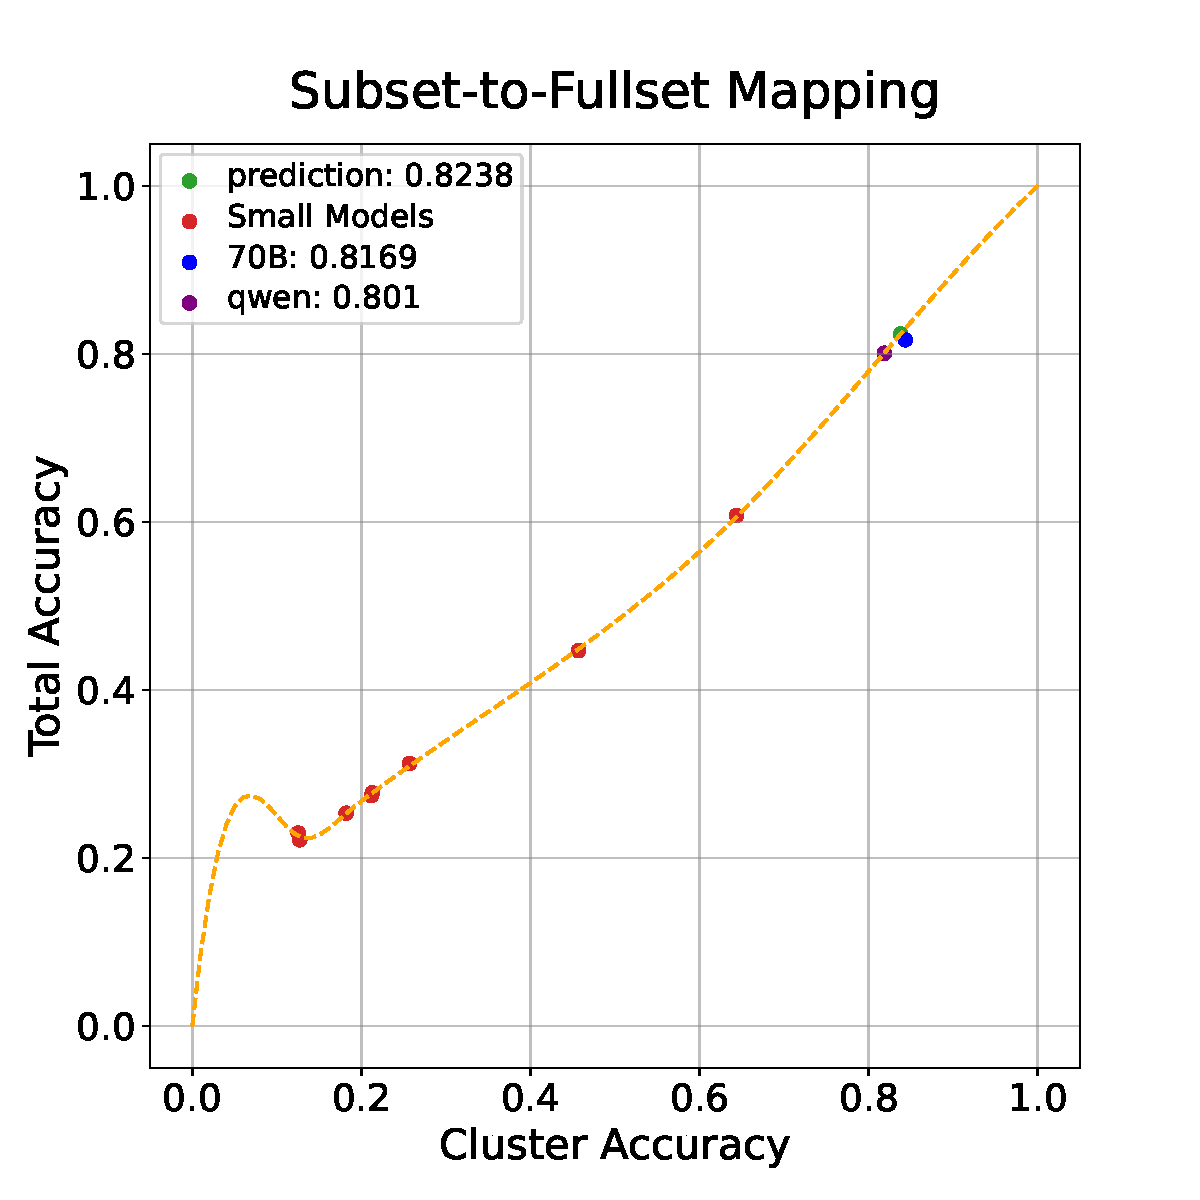
\includegraphics[width=\linewidth]{figures/experiments/mapping/BBH_0.0025_qwen_acc.pdf}
        \caption{$T=0.0025$}\label{subfig:bbh_0.0025}
    \end{subfigure}% 关键：加%取消换行符的隐形空格
    \hfill% 自动填充间距，无固定数值
    \begin{subfigure}[b]{0.22\textwidth}\centering
        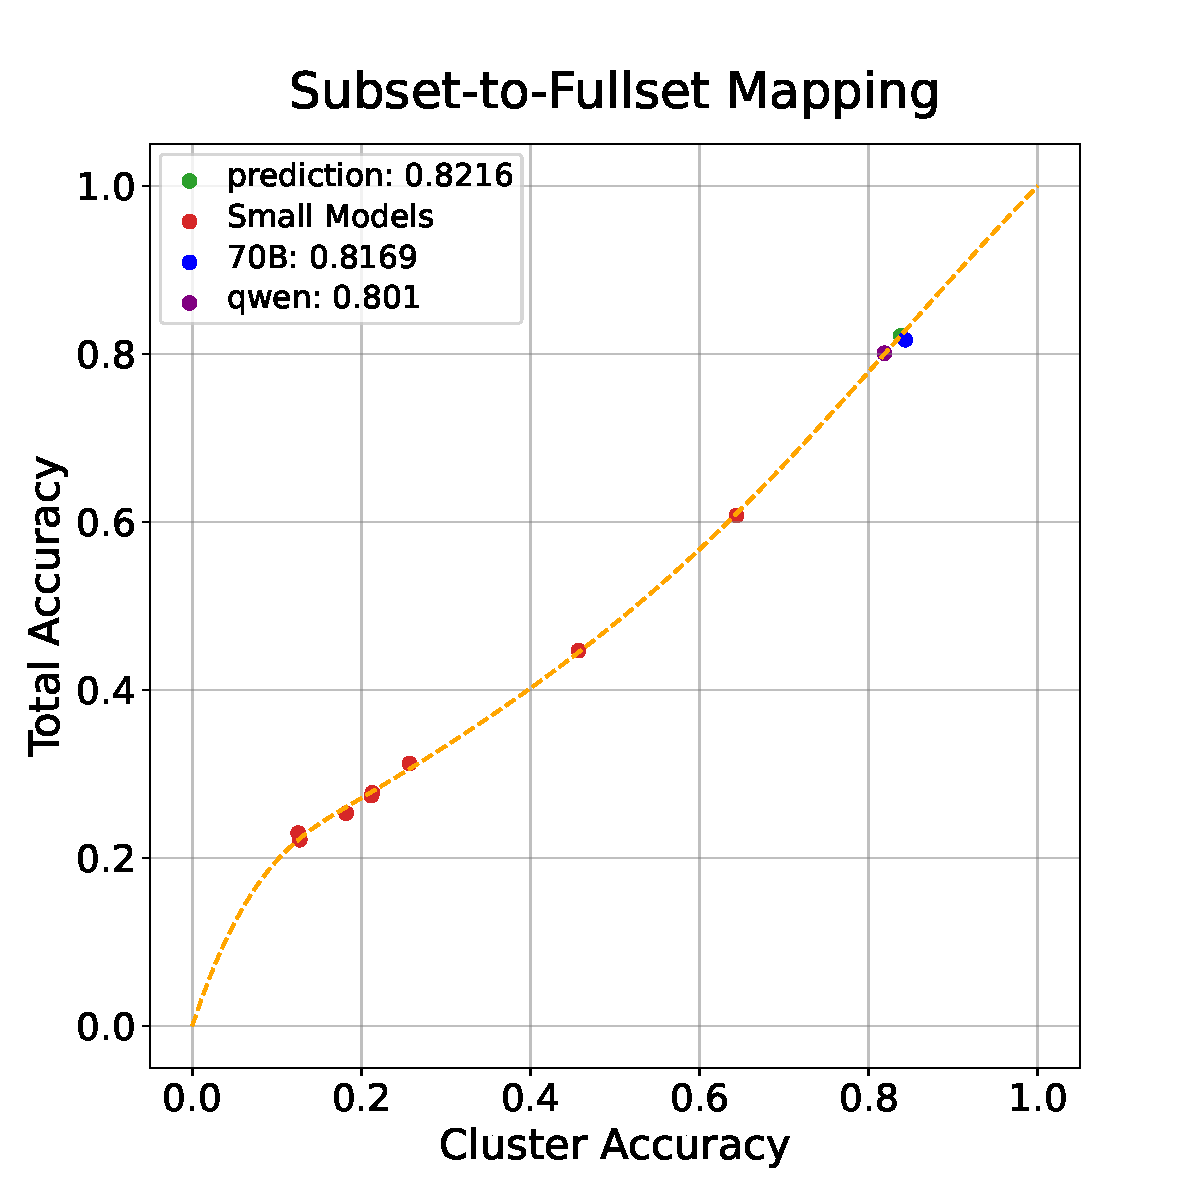
\includegraphics[width=\linewidth]{figures/experiments/mapping/BBH_0.005_qwen_acc.pdf}
        \caption{$T=0.005$}\label{subfig:bbh_0.005}
    \end{subfigure}%
    \hfill
    \begin{subfigure}[b]{0.22\textwidth}\centering
        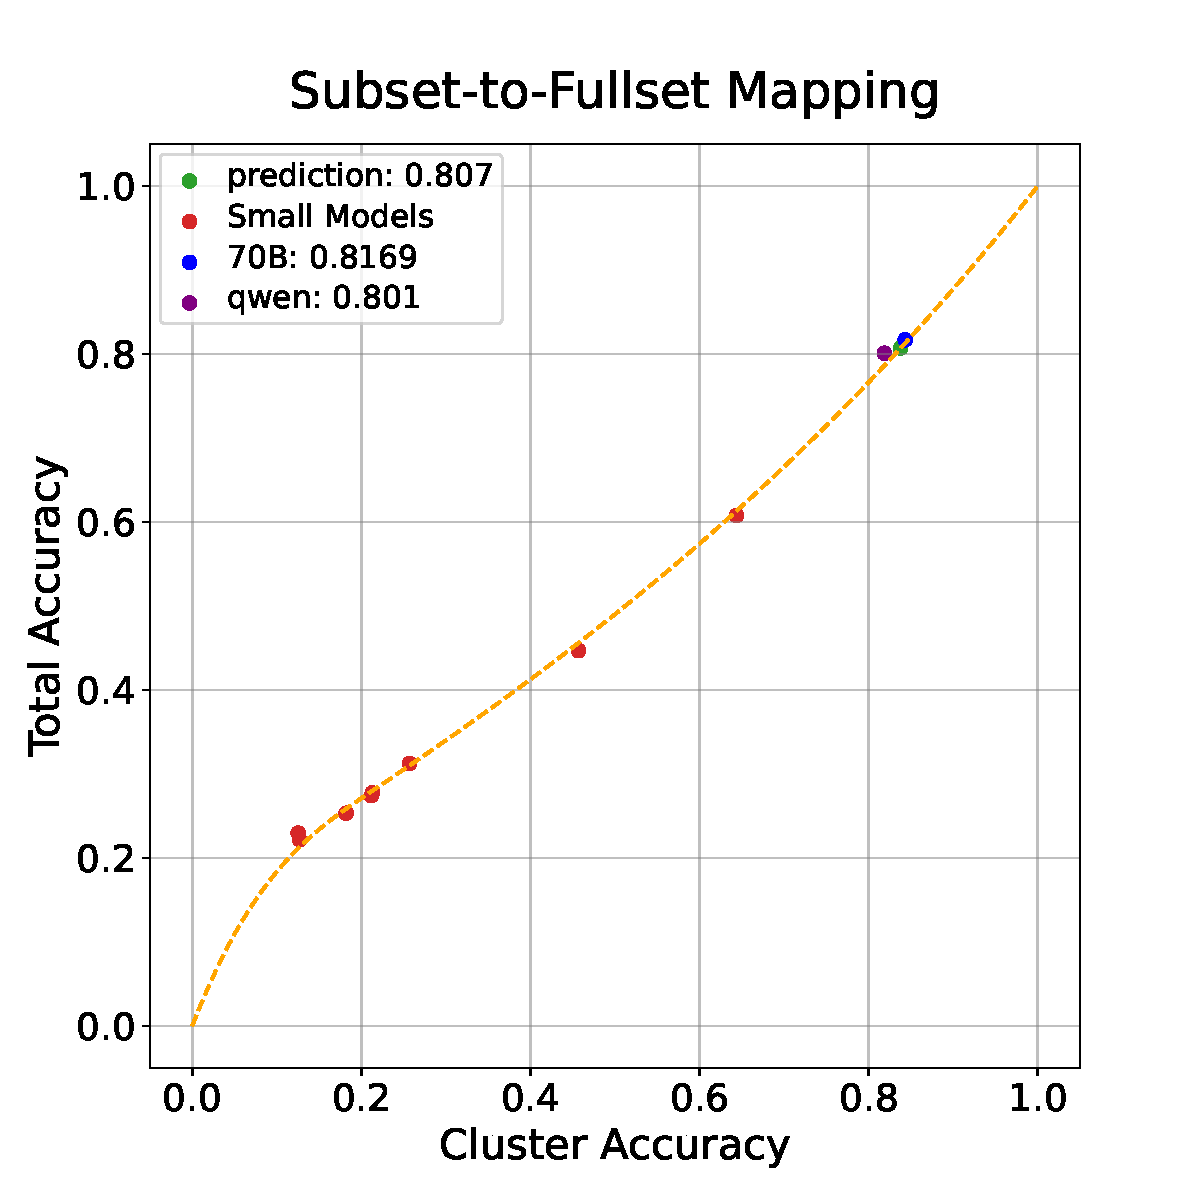
\includegraphics[width=\linewidth]{figures/experiments/mapping/BBH_0.01_qwen_acc.pdf}
        \caption{$T=0.01$}\label{subfig:bbh_0.01}
    \end{subfigure}%
    \hfill
    \begin{subfigure}[b]{0.22\textwidth}\centering
        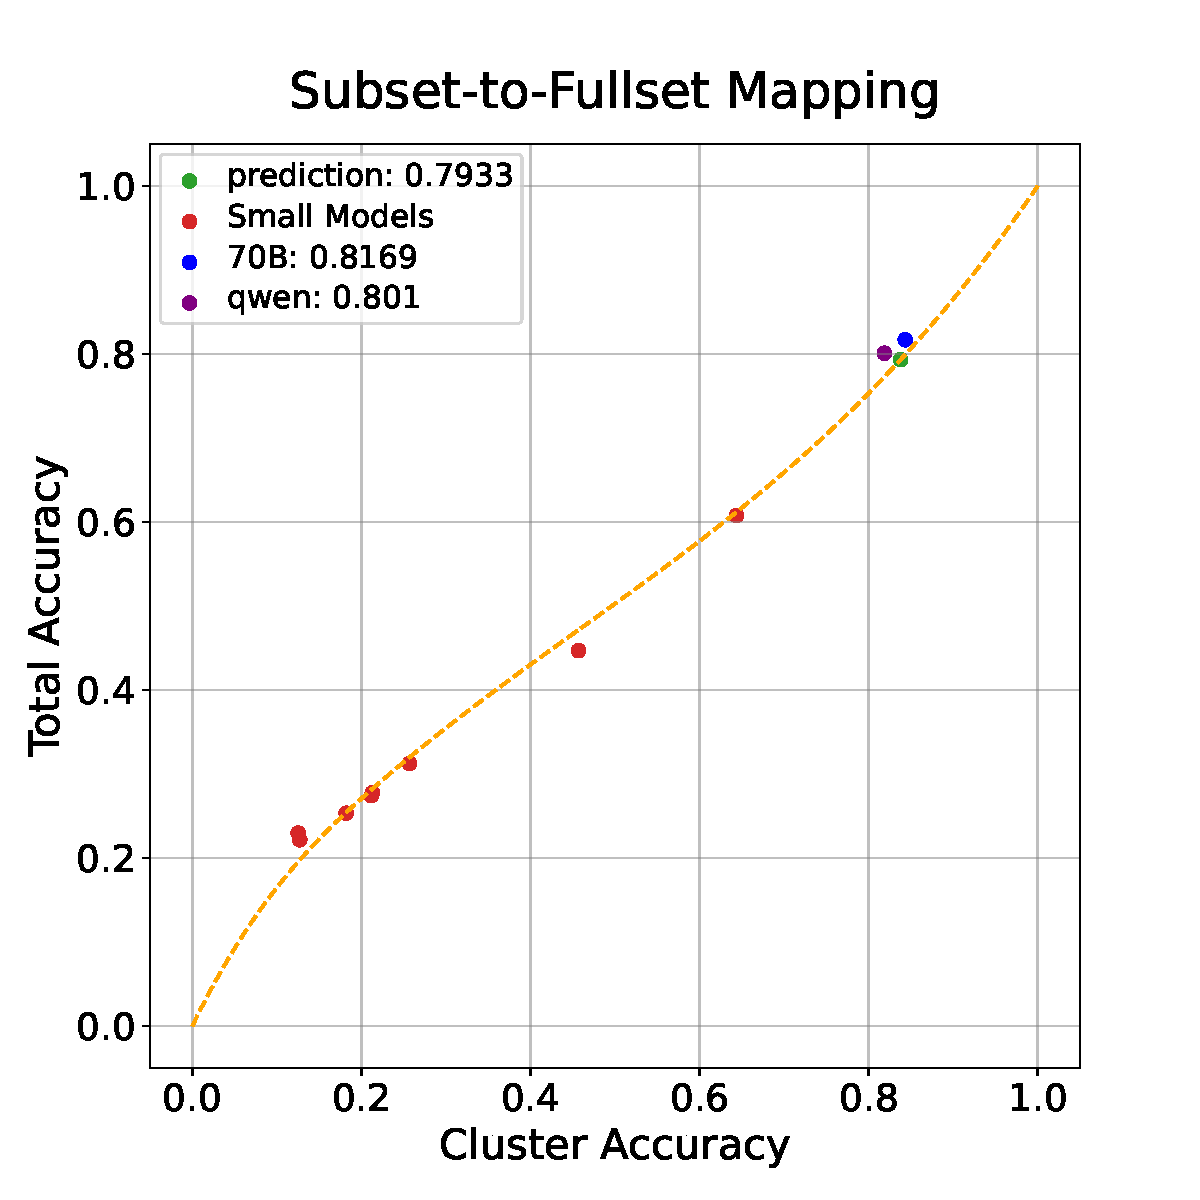
\includegraphics[width=\linewidth]{figures/experiments/mapping/BBH_0.02_qwen_acc.pdf}
        \caption{$T=0.02$}\label{subfig:bbh_0.02}
    \end{subfigure}
    
    \caption{Ablation of RMSE Threshold $T$.}
    \label{fig:RMSE_threshold}
    \vspace{-10pt}
\end{figure*}
% To evaluate different interpolation methods for prediction accuracy, we compared various mathematical approaches. Our baseline method uses quartic polynomial interpolation, which we compare against several alternative approaches, including Cubic spline interpolation, Cubic polynomial interpolation, and Quintic polynomial interpolation

% The comparative results across different benchmarks are shown in \cref{tab:interpolation_results}. We report the prediction error between the real performance of a large model and the mapping result.

% \begin{table}[!t]
% \caption{Comparison of different interpolation methods across benchmarks.}
% \centering
% \small
% \begin{tabular}{c|ccc}
% \toprule
% Prediction Error & BBH & Math & MMLU-pro \\
% \midrule
% Cubic Spline & 0.68 & 1.31 & 1.37 \\
% Cubic Polynomial & 3.38 & 1.12 & 1.35 \\
% Quintic Polynomial & 0.18 & 1.42 & 1.36 \\
% Quartic Polynomial & 1.77 & 1.28 & 1.35 \\
% \midrule 
% Smooth Spline & 2.51 & 0.35 & 0.03 \\
% \bottomrule
% \end{tabular}
% \label{tab:interpolation_results}
% \end{table}

% In \cref{fig:mappling_results_bbh}, we plot the mapping process using different interpolation formulas, where the x-axis represents the predictable subset indices and the y-axis represents the full set indices. The red points are the numerical values to be fitted, green points represent predicted values, purple points represent anchor points, and blue points show the actual performance.

% The prediction performance shows certain robustness across different interpolation methods. We aim to use the simplest possible interpolation function while maintaining low prediction errors. Based on the above results, we observe that the Cubic Polynomial shows larger prediction errors due to underfitting on BBH, while the Cubic Spline exhibits some overfitting. Both Quartic Polynomial and Quintic Polynomial perform well, therefore, we chose the Quartic Polynomial method as it requires fewer fitting parameters.
% \begin{figure}[!t]
%     \centering
%     \begin{minipage}{0.24\textwidth}
%         \centering
%         \includegraphics[width=\textwidth]{figures/experiments/mapping/cubic_spline.pdf}
%         % \caption*{Cubic Polynomial}
%     \end{minipage}
%     \begin{minipage}{0.24\textwidth}
%         \centering
%         \includegraphics[width=\textwidth]{figures/experiments/mapping/cubic_polynomial.pdf}
%         % \caption*{Quartic Polynomial}
%     \end{minipage}
%     \begin{minipage}{0.24\textwidth}
%         \centering
%         \includegraphics[width=\textwidth]{figures/experiments/mapping/quintic_polynomial.pdf}
%         % \caption*{Quintic Polynomial}
%     \end{minipage}
%     \begin{minipage}{0.24\textwidth}
%         \centering
%         \includegraphics[width=\textwidth]{figures/experiments/mapping/quartic_polynomial.pdf}
%         % \caption*{Cubic Spline}
%     \end{minipage}
%     \caption{Performance mapping with different interpolation methods on the BBH evaluation set. The cubic spline is overfitted, and the cubic polynomial method is underfitted. Quartic polynomials and quintic polynomials are comparable, while a quartic polynomial has fewer parameters.}
%     \label{fig:mappling_results_bbh}
% \end{figure}

% \labubu{When the number of small models used for fitting varies, the polynomial form also needs to be adaptively adjusted to ensure the robustness of the mapping. For instance, in the experiment of predicting the 12B model, the scaling function was adjusted from a quartic polynomial to a cubic polynomial to mitigate overfitting.}



\subsection{\labubu{Incorporating Anchor Point in Interpolation Mapping}}
\label{sec:anchor}
We find that the mapping relationship from predictable subset metrics to full evaluation set metrics is similar across models with different training data and architectures. This allows leveraging pre-trained models as "anchors" to refine the mapping and improve final estimation accuracy. \camera{In practice, we simply use an open-source model (Qwen2-72B)} as a refinement anchor. 
%and an in-house MoE model~\citep{lepikhin2020gshardscalinggiantmodels} with the same training data but different architecture (ID anchor). 
We first derive an interpolation curve using only small model metrics and fixed points $(0,0)$, $(1,1)$, then assess anchor compatibility. This shared mapping implies estimable subset metrics are highly correlated with full-set metrics and less prone to interference from other model parameters than loss-intermediate predictions.

We test two configurations:
\begin{itemize}[leftmargin=1.5em]
\item COD (w/o anchor): Full COD pipeline, but no anchor points in the mapping phase;
\item COD (w. anchor): COD method with Qwen2-72B as a refinement anchor;
% \item COD (w. ID anchor): COD with our in-house MoE model as an in-domain anchor.
\end{itemize}
\revise{We list the performance of anchor models and the target model in ~\cref{tab:anchor_info}.}
% 同时，我们在\cref{appdix:anchor_points} MATH与MMLU-pro两个评估集上对比了引入与不引入Anchor point参与Mapping的差异。MATH评估集在可外推子集与全集具有明显差异，添加Anchor point后显著提升了拟合与预测效果。而MMLU-pro评估集可预估子集占比高，可预估子集指标与全集基本接近，是否引入Anchor point差异不大。
\camera{In \cref{appdix:anchor_points}, we also compare the differences of using anchor points in the Mapping stage against not using them on two evaluation datasets: MATH and MMLU‑pro.
The MATH dataset shows a clear discrepancy between the predictable subset and the full set, and adding anchor points significantly improves the fitting and prediction performance.
In contrast, the MMLU‑pro dataset has a high proportion of predictable instances (listed in \cref{sec:ablation_extrapolation}), and its metrics for the predictable subset are close to those of the full set, so introducing anchor points yields little difference.}

\begin{table*}[h]
\centering
\caption{Performance comparison among the target model and anchor models.}
\label{tab:benchmark_results}
\resizebox{\textwidth}{!}{%
\begin{tabular}{lcccccccc}
\toprule
\textbf{Model} & \textbf{GSM8K} & \textbf{MATH} & \textbf{BBH} & \textbf{TriviaQA} & \textbf{MBPP} & \textbf{AGIEval} & \textbf{DROP} & \textbf{MMLU-pro} \\
\midrule
70B-Dense & 88.55 & 48.02 & 81.69 & 80.66 & 68.00 & 58.20 & 76.82 & 57.28 \\
Qwen2-72B & 88.63 & 53.08 & 80.10 & 84.23 & 71.60 & 64.16 & 77.56 & 56.93 \\
% 2.5B-MoE  & 86.66 & 50.36 & 79.60 & 72.17 & 70.60 & 58.70 & 74.30 & 57.37 \\
\bottomrule
\end{tabular}%
}
\label{tab:anchor_info}
\end{table*}

\begin{figure*}[!t]
    \centering
    \begin{subfigure}[b]{0.24\textwidth}\centering
        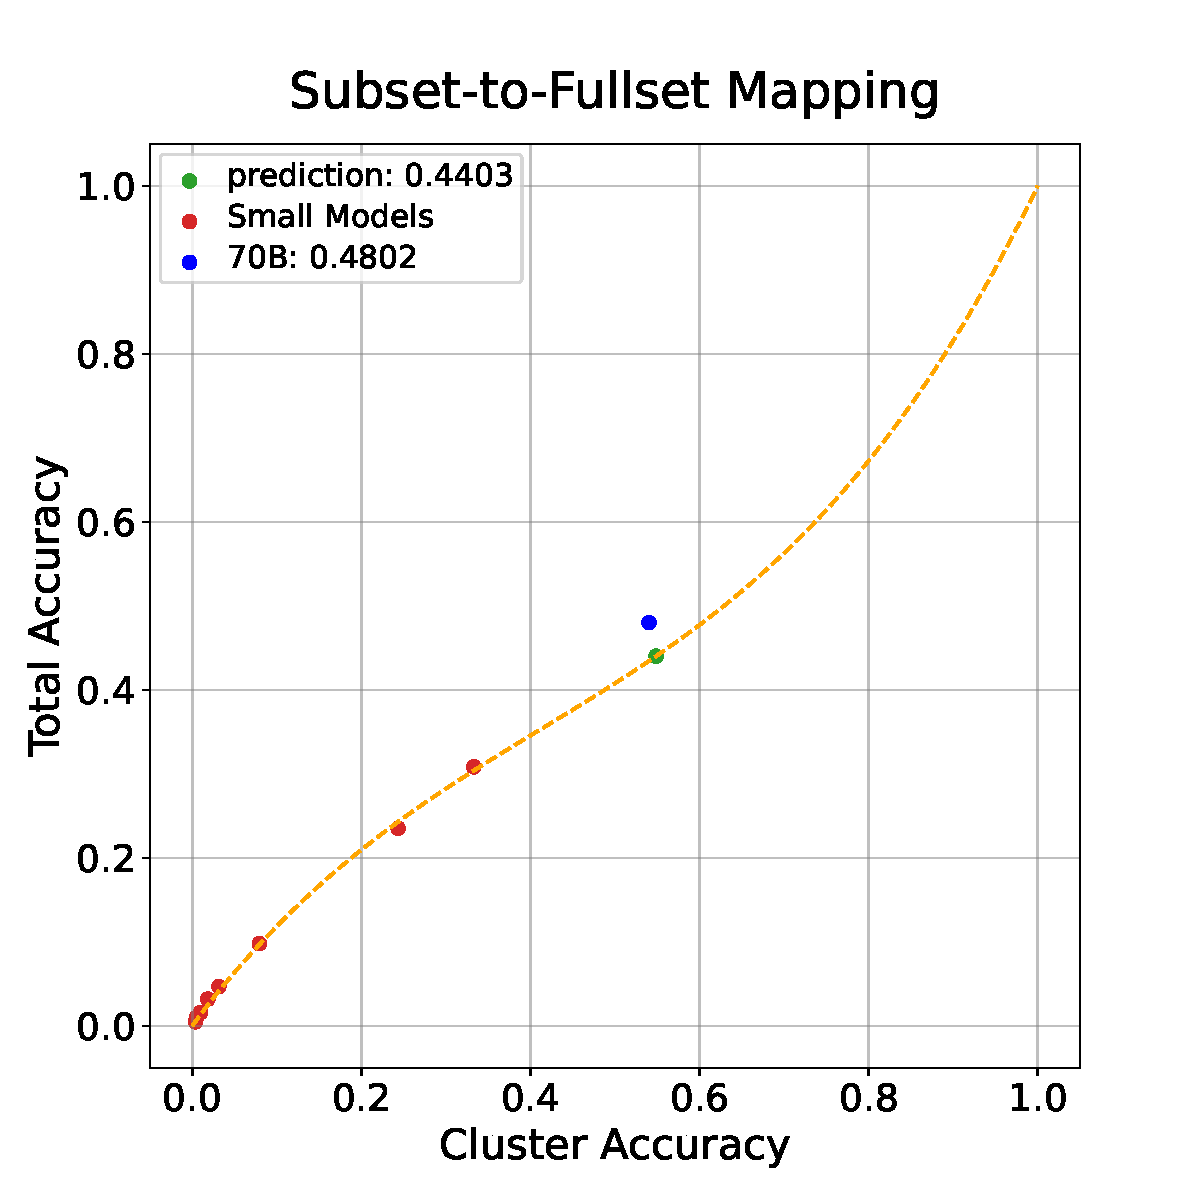
\includegraphics[width=\linewidth]{figures/experiments/mapping/MATH_0.005_None_acc.pdf}
        \caption{\small{MATH w/o anchor}}\label{subfig:bbh_0.0025}
    \end{subfigure}% 关键：加%取消换行符的隐形空格
    \hfill% 自动填充间距，无固定数值
    \begin{subfigure}[b]{0.24\textwidth}\centering
        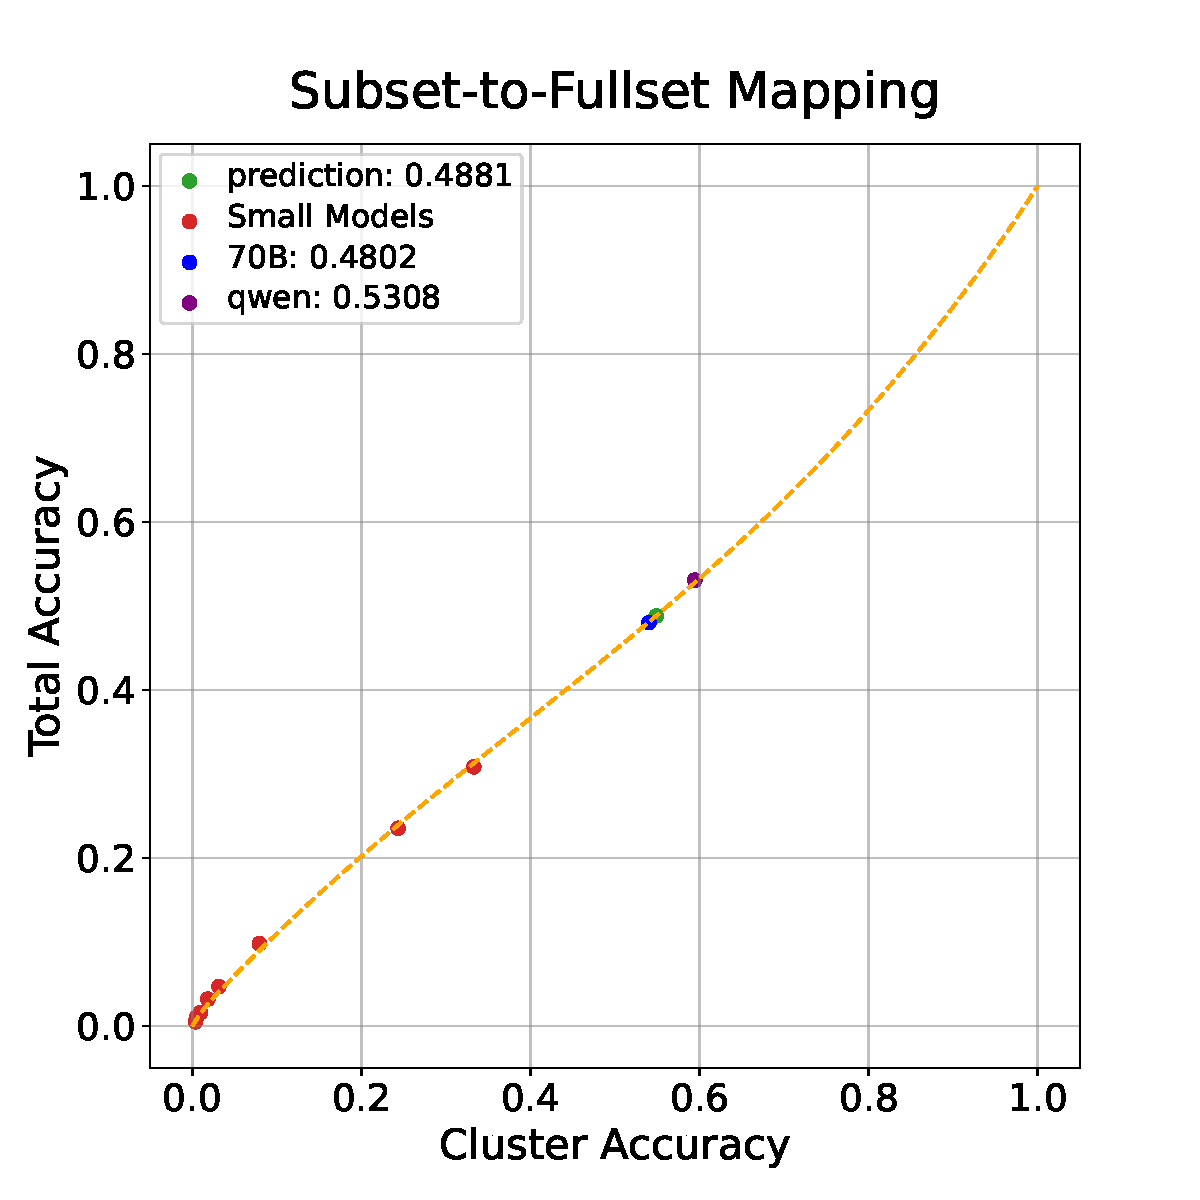
\includegraphics[width=\linewidth]{figures/experiments/mapping/MATH_0.005_qwen_acc.pdf}
        \caption{\small{MATH w/ anchor}}\label{subfig:bbh_0.005}
    \end{subfigure}%
    \hfill
    \begin{subfigure}[b]{0.24\textwidth}\centering
        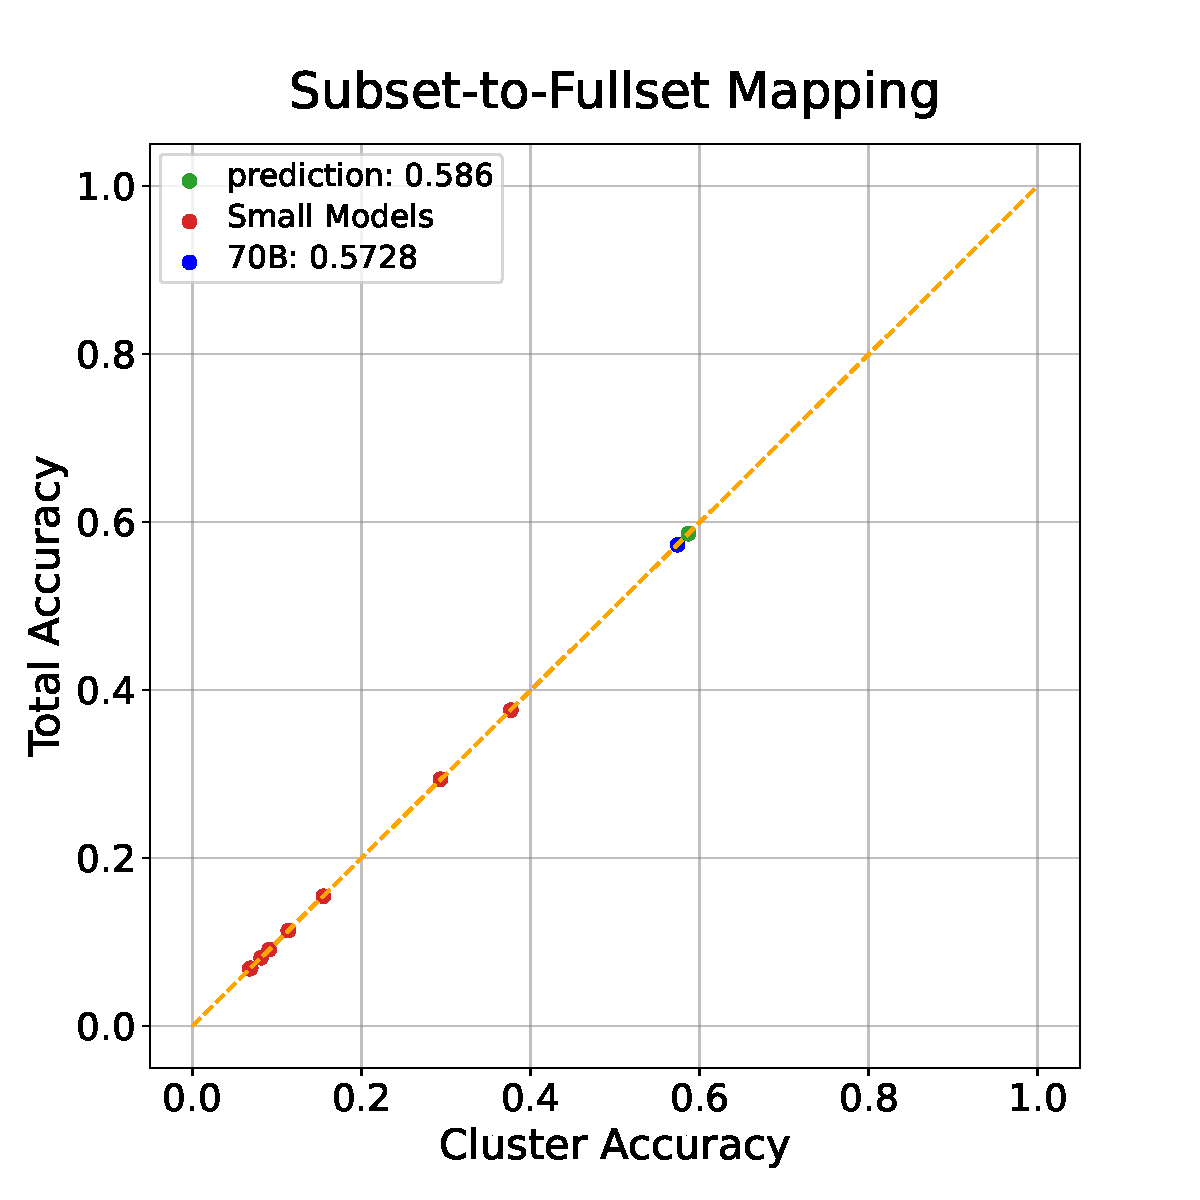
\includegraphics[width=\linewidth]{figures/experiments/mapping/MMLUpro_0.005_None_acc.pdf}
        \caption{\small{MMLUpro w/o anchor}}\label{subfig:bbh_0.01}
    \end{subfigure}%
    \hfill
    \begin{subfigure}[b]{0.24\textwidth}\centering
        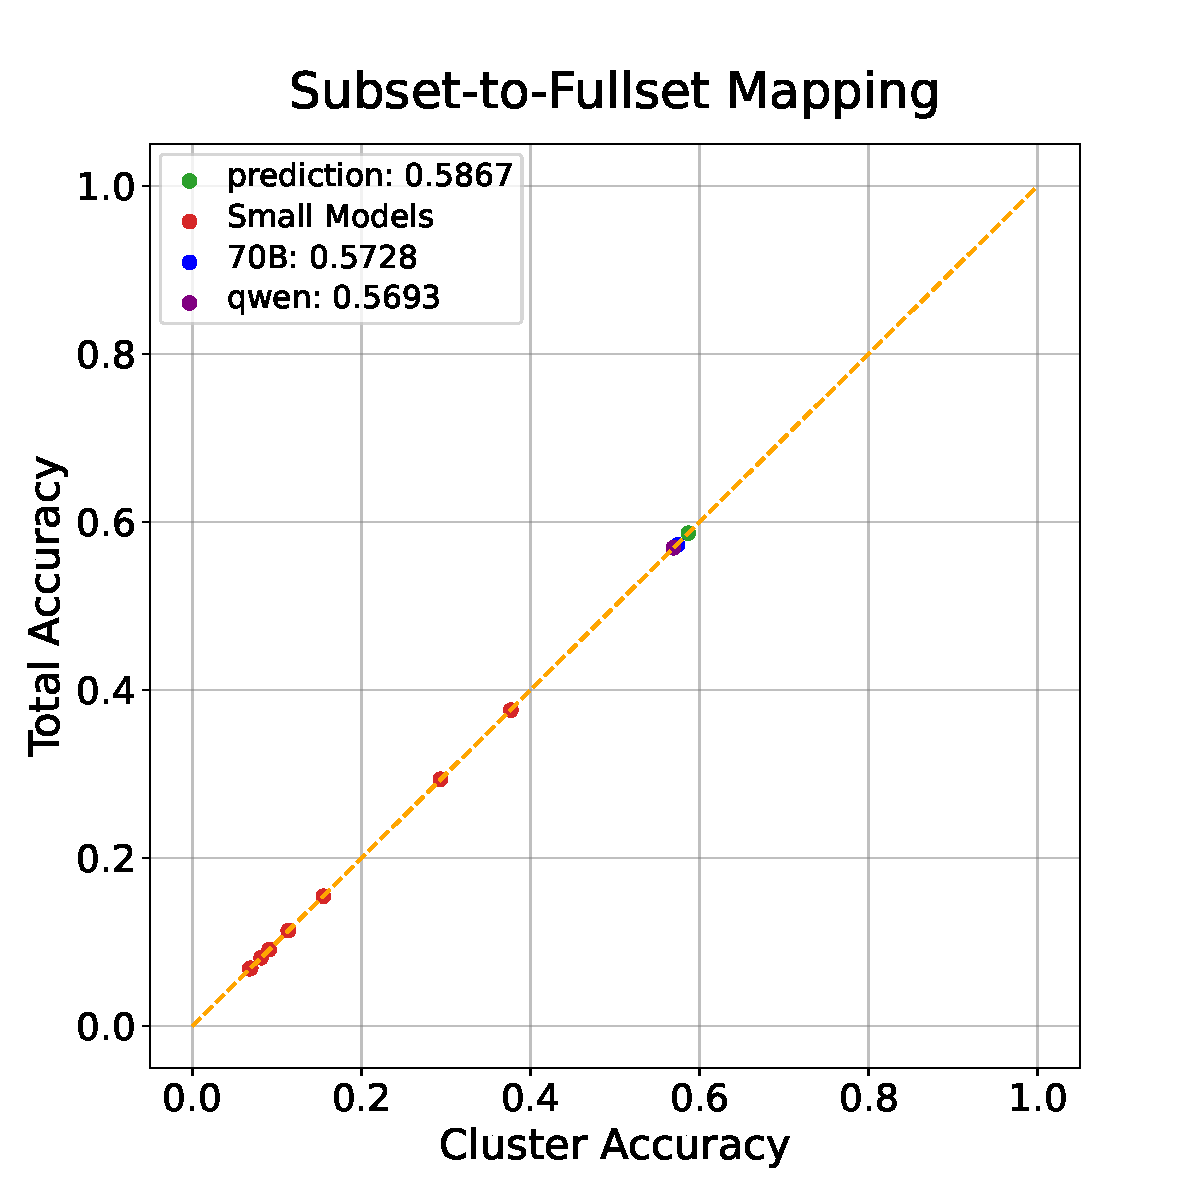
\includegraphics[width=\linewidth]{figures/experiments/mapping/MMLUpro_0.005_qwen_acc.pdf}
        \caption{\small{MMLUpro w/ anchor}}\label{subfig:bbh_0.02}
    \end{subfigure}
    \caption{\camera{Effectiveness of mapping with or without anchor points.}}
    \label{appdix:anchor_points}
\label{fig:anchor_compare}

\end{figure*}

\begin{table*}[]
\centering
\small
\caption{Influence of anchor points in the mapping stage on prediction error (\%). Errors < 2\% are considered accurate (green), while errors > 5\% are considered invalid (red). ↓ indicates lower is better.}
\setlength{\tabcolsep}{2.5pt}
\resizebox{\textwidth}{!}{% 自适应页面宽度
\begin{tabular}{c|c|cc|c*{7}{c}}
\toprule
\multirow{2}{*}{Setting} & \multirow{2}{*}{Method} & \multicolumn{2}{c|}{Overall} & \multicolumn{8}{c}{Individual Task Sets} \\
\cmidrule(lr){3-4} \cmidrule(lr){5-12}
& & Mean$\downarrow$ & Max$\downarrow$ & GSM8k & MATH & BBH & TriviaQA & MBPP & AGIEval & DROP & MMLU-pro \\

% & w. ID anchor & {1.63} & {2.38} & {2.23} & {1.28} & {1.77} & {1.64} & {2.19} & {2.38} & {0.23} & {1.35} \\
\midrule
\multirow{2}{*}{End-to-end(exp)} & w/o anchor & 3.10 & 6.00 & 4.00 & 3.86 & \greenhl{0.64} & \greenhl{0.68} & \greenhl{1.75} & \redhl{6.00} & 4.11 & 3.72 \\
& w/ anchor & 3.08 & 6.42 & \greenhl{0.56} & \redhl{5.75} & \greenhl{0.93} & 2.25 & 2.82 & \redhl{6.42} & \greenhl{1.10} & 4.80 \\
% & w/ ID anchor & 9.55 & 21.85 & 4.76 & 16.05 & 10.56 & 1.89 & 8.24 & 10.63 & 2.41 & 21.85 \\
\midrule
\multirow{2}{*}{End-to-end(BNSL)} & w/o anchor & 5.17 & 13.05 & 4.23 & \redhl{5.88} & \redhl{13.05} & \redhl{5.86} & 2.55 & \greenhl{0.82} & \greenhl{1.53} & \redhl{7.42} \\
& w/ anchor & 3.60 & 6.65 & \greenhl{0.18} & \redhl{5.77} & \greenhl{1.28} & 4.17 & 4.22 & \redhl{6.65} & \greenhl{1.43} & \redhl{5.10} \\
% & w/ ID anchor & 15.34 & 30.49 & 6.32 & 24.04 & 14.25 & 5.72 & 15.86 & 15.99 & 10.06 & 30.49 \\
\midrule
\multirow{2}{*}{COD} & w/o. anchor & 2.65 & 4.98 & 3.10 & 3.99 & \greenhl{0.97} & 2.38 & \greenhl{1.59} & 4.98 & 2.86 & \greenhl{1.32} \\
& w. anchor & \textbf{1.55} & \textbf{2.68} & 2.68 & \greenhl{0.79} & \greenhl{0.47} & \greenhl{1.97} & 2.42 & \greenhl{1.64} & \greenhl{1.05} & \greenhl{1.39} \\
\bottomrule
\end{tabular}}
\label{tab:ablation_study}
% \vspace{-10pt}
\end{table*}

% %我们同样给End-to-end与BNSL等Baseline方法添加anchor point作为对照，添加的OOD与ID anchor都与COD方法相同。在实践中，我们把anchor point直接参与拟合外推公式。
% \cref{tab:ablation_study} shows that COD method incorporating either OOD or ID anchors consistently enhances prediction accuracy. 
% % 然而End-to-end与BNSL等基线方法并没有从添加anchor point中取得提升。
% This suggests a stable correlation between predictable subset and full-set metrics across diverse models, enabling the use of existing model evaluations to improve predictions for new models. 
% % 相对的，End-to-end与BNSL只能把anchor point作为拟合点，仅能让预测目标靠近anchor point的Scaling趋势，但不同训练数据和结构训练的模型Scaling趋势具有显著差异，在不同能力分向上表现差异性大，从而无法获取有效预估。
% Furthermore, since our clustering identifies intrinsic properties of evaluation sets, the derived predictable subsets are applicable to new models. Additional ablations on the interpolation method (\cref{sec:interpolation_ablation}) confirms quartic functions are suitable.

\camera{To facilitate a direct comparison, we also apply the anchor point to baseline methods including End-to-end(exp) and End-to-end(BNSL), using the same anchor as in the COD method. In practice, the anchor points are directly incorporated into the fitting process of the extrapolation formula.}

\camera{\cref{tab:ablation_study} shows that the COD method incorporating anchor consistently enhances prediction accuracy. However, the End-to-end(exp) and End-to-end(BNSL) baselines failed to derive any benefit from the addition of anchor points. 
This suggests a stable correlation between the predictable subset and full-set metrics across diverse models, enabling the use of existing model evaluations to improve predictions for new models. 
In contrast, End-to-end(exp) and End-to-end(BNSL) treat anchor points merely as fitting samples, aligning the prediction target solely with the scaling trend of the anchors. 
Yet, scaling trends differ significantly across models trained on different data and architectures, manifesting as high variance across different capability dimensions; consequently, these methods fail to produce effective estimations. 

Furthermore, since our clustering identifies intrinsic properties of evaluation sets, the derived predictable subsets are applicable to new models.}
% Additional ablations on the interpolation method (\cref{sec:interpolation_ablation}) confirm that quartic functions are suitable.





\section{Experimental Settings and Training Recipe}
\label{append:setting}
\noindent\textbf{Training recipe.}
To establish performance predictions for large language models, we conduct systematic experiments with a suite of smaller-scale models across different parameter counts. All our models are trained from scratch on a corpus of text data. We do not fix the data budget for all models; instead, we maintain a consistent Data-to-CPT (Compute Per Token) ratio for all models, as mentioned in \cref{sec:exp_setups}. We list model configurations in \cref{tab:model_configs_dense}.

We adopt the in-house training data that comprises multilingual text corpora, with increased weighting for domains such as STEM, code, and general knowledge, following Llama3~\citep{grattafiori2024llama}, Deepseek-v2~\citep{liu2024deepseek}, Fineweb-EDU~\citep{lozhkov2024fineweb}, etc. We apply several de-duplication methods and data cleaning mechanisms to each data source to ensure high-quality tokens.

The model architecture is consistent with Llama3.1~\citep{grattafiori2024llama}, incorporating Grouped-Query Attention (GQA)~\citep{ainslie2023gqa}, SwiGLU activation function~\citep{shazeer2020glu}, RMSNorm~\citep{zhang2019root} with Pre-normalization, etc. The models are trained using $BF16$ precision with a sequence length of $8192$ and a RoPE~\cite{su2024roformer} base of $500,000$. We employ the AdamW optimizer with $\beta=(0.9,0.95)$, a weight decay of $0.1$, and a dropout rate of $0.1$.

All models are trained on a constant learning rate scheduler with a few-step warmup stage. To determine the learning rate and batch size, we adopt the hyperparameter scaling laws from \citet{liu2024deepseek}. Specifically, the optimal learning rate $\eta_{\mathrm{opt}}$, and the optimal batch size $B_{\mathrm{opt}}$ are defined as power laws of the compute, measured in FLOPs: $\eta_{opt}=a_1\cdot C^{-b_1}$ and $B_{opt}=a_2\cdot C^{b_2}$, where $a_1$, $b_1$, $a_2$, $b_2$ are parameters to be fitted. We perform a grid search on our small models to identify their optimal learning rates and batch sizes, and then extrapolate these findings to the bigger models.
% \noindent\textbf{Model Specifications}

\begin{table}[!t]
\centering
\small
\caption{Model architecture specifications across different sizes.}
\setlength{\tabcolsep}{2.5pt}
\begin{tabular}{c|ccccccccc}
\toprule
 & 122M & 238M & 411M & 652M & 973M & 1.9B & 7B & 12B & 70B (Target) \\
\midrule
Param. (M) & 122 & 238 & 411 & 652 & 973 & 1,901 & 6,980 & 12,022 & 68,452 \\
Compute Per Token (B) & 1.535 & 2.684 & 4.275 & 6.378 & 9.060 & 16.436 & 54.761 & 91.609 & 475.131 \\
Tokens (B) & 26 & 45 & 72 & 108 & 153 & 277 & 923 & 1,544 & 8,012 \\
Continue-Trained Tokens (B) & 3 & 5 & 8 & 12 & 18 & 33 & 114 & 191 & 1,000 \\
Model Dimension & 1,024 & 1,280 & 1,536 & 1,792 & 2,048 & 2,560 & 4,096 & 4,608 & 8,192 \\
FFN Dimension & 3,584 & 4,480 & 5,376 & 6,272 & 7,168 & 8,960 & 14,336 & 16,128 & 28,672 \\
Heads & 8 & 10 & 12 & 14 & 16 & 20 & 32 & 36 & 64 \\
KV Heads & 8 & 10 & 12 & 14 & 16 & 20 & 8 & 12 & 8 \\
\bottomrule
\end{tabular}
\label{tab:model_configs_dense}
\end{table}

\anno{\noindent\textbf{Training Resources.} The 7B dense model is trained on 923B tokens, consuming 52,800 H800 GPU-hours. The computational resources used for the other models can be estimated proportionally based on their respective compute requirements.}

\anno{\noindent\textbf{Evaluation settings and protocol.}}
We conducted performance scaling estimation experiments across eight major LLM evaluation sets. These evaluation sets span a diverse range of capabilities, including Math, Reasoning, Knowledge, Coding, Reading, and general abilities. All pretrained LLMs were evaluated using a few-shot methodology to obtain the performance metrics. Detailed information is provided in~\cref{tab:evaluation_info}. \anno{Our evaluation methodology aligns with that used for the Llama3~\citep{grattafiori2024llama} pre-trained models. We assess the models' capabilities directly through few-shot text completion tasks without any instruction tuning or Supervised Fine-Tuning (SFT). This evaluation method is chosen because even a small amount of SFT data can significantly influence performance on downstream tasks, thereby not reflecting the inherent capabilities of the pre-trained model itself.}

\anno{\noindent\textbf{Software Framework.}
All models are trained using the Megatron framework. The evaluation code is an in-house implementation designed to be consistent with the Llama3~\citep{grattafiori2024llama} evaluation methodology.}

\label{appix:exp_settings}
\begin{table}
\centering
\small
\caption{Information of evaluation datasets.}
\setlength{\tabcolsep}{3pt}
\begin{tabular}{c|ccc}
\toprule
Dataset & Domain & \#Questions & \#Shots \\
\midrule
GSM8K & Math & 1,319 & 8 \\
MATH & Math & 5,000 & 4 \\
BBH & Reasoning & 6,511 & 3 \\
TriviaQA & Knowledge & 17,944 & 5 \\
MBPP & Coding & 500 & 3 \\
AGIEval& Comprehensive & 8,063 & 5 \\
DROP & Reading & 9,536 & 3 \\
MMLU-pro  & Comprehensive & 12,032 & 5 \\
\bottomrule
\end{tabular}
\label{tab:evaluation_info}
\end{table}

% \renewcommand{\thefigure}{D\arabic{figure}}
% \renewcommand{\thetable}{D\arabic{table}}
% \renewcommand{\theproposition}{D.\arabic{proposition}}
% \setcounter{table}{0} 
% \setcounter{figure}{0} 

% \section{Additional Prediction Results for a Medium-size Model}
% \label{append:12B}
% \anno{The COD method is also effective for predicting the capabilities of medium-size language models. To demonstrate this, we conducted an experiment to predict the performance of a 12B model using source models ranging from 122M to 1.9B parameters. This setup maintains a similar ~6$\times$ parameter-size ratio as our main experiment (predicting 70B from models up to 12B).

% For this experiment, clustering relied exclusively on the passrate@100 data from the 122M to 1.9B source models to prevent data leakage from the target model. The results in~\cref{tab:12B_results} show that COD is more robust and less demanding on the size of source models compared to the baselines. For instance, the baseline methods perform poorly on the BBH benchmark, In contrast, COD accurately captures the trend of accuracy growth as compute increases and yields precise extrapolations. We will include a plot of this curve in the main text to visually demonstrate the clear advantage of COD.

% The prediction errors of all methods for the 12B model are significantly higher than those for the 70B model reported in~\cref{subsec:Prediction_Experiments}. Extrapolation accuracy improves when larger source models are employed for fitting, as a greater number of samples have ``emerged''. If the largest source model is excessively small, numerous samples remain ``unemerged'', resulting in substantial errors when extrapolating to a significantly larger model.}

% \begin{table*}[!t]
% \small
% \setlength{\tabcolsep}{1.8pt} % 保持原列间距设置
% \centering
% \caption{Absolute prediction error (\%) on evaluation sets for predicting the performance of the 12B model. Errors < 2\% are considered accurate (green), while errors > 5\% are considered invalid (red). $\downarrow$ indicates lower is better.}
% \begin{tabular}{c|c|cc|cc|cc|cc} % 列结构：任务/指标 | 真值 | 4组[Prediction|Error]
% \toprule
% \multirow{2}{*}{Task Sets/Metrics} & \multirow{2}{*}{Ground Truth} & \multicolumn{2}{c|}{\textbf{Loss-intermediate}} & \multicolumn{2}{c|}{\textbf{End-to-end}} & \multicolumn{2}{c|}{\textbf{BNSL}} & \multicolumn{2}{c}{\textbf{COD}} \\
% \cmidrule(lr){3-10} % 分隔线覆盖所有方法的Prediction-Error列
% & & Prediction & Error & Prediction & Error & Prediction & Error & Prediction & Error \\
% \toprule
% \multicolumn{10}{c}{\textbf{Overall Metrics}} \\ % 横向标题适配10列
% \midrule
% Mean & - & - & 14.92 & - & 10.52 & - & 17.42 & - & \textbf{4.68} \\
% Max & - & - & 23.82 & - & 24.43 & - & 28.26 & - & \textbf{10.39} \\
% \midrule
% \multicolumn{10}{c}{\textbf{Individual Task Sets}} \\ % 横向标题适配10列
% \midrule
% GSM8k & 70.47 & 60.86 & \redhl{9.61} & 63.66 & \redhl{6.81} & 80.99 & \redhl{10.52} & 60.08 & \redhl{10.39} \\
% MATH & 30.85 & 41.53 & \redhl{10.68} & 34.36 & 3.51 & 49.26 & \redhl{18.41} & 28.48 & 2.37 \\
% BBH & 60.76 & 36.94 & \redhl{23.82} & 36.33 & \redhl{24.43} & 36.10 & \redhl{24.66} & 57.751 & 3.05 \\
% TriviaQA & 58.84 & 68.42 & \redhl{9.57} & 59.88 & \greenhl{1.04} & 87.10 & \redhl{28.26} & 57.92 & \greenhl{0.93} \\
% MBPP & 47.80 & 28.53 & \redhl{19.27} & 36.51 & \redhl{11.29} & 27.95 & \redhl{19.85} & 44.50 & 3.30 \\
% AGIEval & 44.13 & 33.91 & \redhl{10.22} & 35.40 & \redhl{8.74} & 34.12 & \redhl{10.01} & 47.53 & 3.40 \\
% DROP & 54.35 & 35.05 & \redhl{19.30} & 37.19 & \redhl{17.16} & 36.73 & \redhl{17.62} & 63.50 & \redhl{9.14} \\
% MMLU-pro & 37.60 & 20.74 & \redhl{16.86} & 26.41 & \redhl{11.20} & 27.59 & \redhl{10.01} & 42.42 & 4.82 \\
% \bottomrule
% \end{tabular}
% \label{tab:12B_results}
% % \vspace{-10pt}
% \end{table*}


\section{Performance Prediction for Continue-Pretrained LLMs}
\label{sec:ppct}
Leading industry pre-trained LLMs (e.g., Deepseek-v3~\citep{deepseekai2025deepseekv3technicalreport}, Llama3~\citep{grattafiori2024llama}, Qwen-2.5~\citep{qwen2.5}) adopt the Continual Training (CT) strategy of concentrating high-quality data towards the end of the pre-training process. This phase is typically accompanied by learning rate decay, enabling the model to fully absorb this high-quality data. Due to significant changes in data distribution and the learning rate schedule, this approach often yields substantial improvements in metrics. Predicting a large model's final capability based solely on its performance during a ``stable'' phase with consistent data distribution does not reflect its ultimate capability. Therefore, we supplement this by providing metric predictions for the high-quality CT phase.

The relationship between model parameter scale and the volume of CT tokens is listed in~\cref{tab:model_configs_dense}. We conduct the same COD pipeline for CT models. We control the data distribution of the stable and decay phases for various smaller models, as well as their token-to-parameter ratio, to be consistent with the large model targeted for prediction. The last checkpoint is used for evaluation. Based on prior clustering labels, we perform fitting, extrapolation, and mapping to obtain the predicted performance for the large model. 

\begin{table}[!h]
\centering
\caption{Predicted vs. actual metrics for an LLM with 70B parameters after high-quality continued pretraining. Errors < 2\% are considered accurate (green)}
\label{tab:ct_results}
\begin{tabular}{lccc}
\toprule
Evaluation Set & Predicted Metric & Actual Metric & Prediction Error \\
\midrule
GSM8k          &    93.10        & 91.81         &    \greenhl{1.29}        \\
MATH           &    56.35        & 52.68         &    3.67         \\
BBH            &    83.05       &  85.32         &    2.27          \\
TriviaQA       &    79.29        & 84.05         &    4.76          \\
MBPP           &    72.42        & 73.20         &    \greenhl{0.78}          \\
AGIEval        &    63.22        & 64.18         &    \greenhl{0.96}          \\
DROP           &    82.34        & 81.39         &    \greenhl{0.95}          \\
MMLU-pro       &    62.11        & 59.34         &    2.77          \\
\bottomrule
\end{tabular}
\end{table}



% 我们注意到MATH, GSM8k与TriviaQA具有相对较大的预测误差，并认为造成预测不准确的原因可能有两类：
% 1. CT数据与评估集具有明显相关性，例如数学类评估集，少量训练即可带来大量指标提升。此时小模型指标的波动性较大，同时大模型能力上限也更收到训练数据质量约束，导致Scaling规律发生变化。
% 2. CT数据具有偏向性，部分评估集不能从中获得效果提升，例如TriviaQA, 让CT阶段前后的指标为波动关系，降低了小模型指外推的准确性。

Results listed in~\cref{tab:ct_results} show that the proposed COD method achieves an average prediction error of \camera{2.18}\%. We observe that MATH and TriviaQA exhibit relatively large prediction errors. We hypothesize that there are two main categories of reasons for this inaccuracy:

\begin{enumerate}[label=\arabic*.,leftmargin=1.5em]
    \item The CT data and the evaluation sets possess a significant correlation. For example, in math-related evaluation sets, a modest amount of training can yield substantial improvements in performance metrics. In such scenarios, the metrics for smaller models tend to show greater volatility and have inaccurate evaluations.
    \item The CT data exhibits inherent distribution bias, such that certain evaluation sets, such as TriviaQA, do not derive performance gains from it. This leads to potential significant fluctuations in the metrics after the CT phase, thereby diminishing the accuracy of extrapolating to larger models.
\end{enumerate}


\section{Difficulty Distribution of Predictable Subset}
\label{sec:difficulty_distribution}
% 我们观察在不同难度层级上的可预估子集任务占比，我们把不同评估集的可预估子集与全集的难度分布绘制在了~\cref{fig:diff_dist}中。我们采用12B模型的得分做为难度分级的依据。可以看出，在MMLU-pro, GSM8k评估集上，可预估子集占比较大。说明该评估集大部分题目Scaling性质良好。而在Math评估集上，很多得分接近0的困难题目不在可预估子集中，这部分题目的预估则需要Mapping阶段进行修正。同时BBH在各个难度分布上可预估子集的占比接近，这是因为BBH有部分题目随Compute提升的提升收益较小，表现出震荡走势。

% 我们可以通过可预估子集的占比来评估测试集质量。对于可预估子集占比更大的评估集，我们在小模型上进行的实验结论会更加可靠。
% 同时在我们构建评估集时，对不可预估类簇进行筛查或补充。保证每一类难度特征题目的最小数量，以此降低指标波动性。
We analyze the proportion of predictable subset tasks across different difficulty levels. 
The difficulty distributions of predictable subset versus complete sets for different evaluation benchmarks are illustrated in \cref{fig:diff_dist}. 
We use the scores from the 12B model as the basis for difficulty classification. 
The results show that MMLU-pro and GSM8k evaluation sets have larger proportions of predictable subsets, indicating that most questions in these datasets exhibit good performance scaling properties. In contrast, many difficult questions with near-zero scores in the MATH evaluation set fall outside the predictable subset, requiring adjustment during the mapping phase. 
Meanwhile, BBH exhibits consistent proportions of its predictable subset across varying difficulty levels, as some questions display oscillatory patterns with limited improvement, even with increased computational resources.


The proportion of the predictable subset can serve as a metric for assessing evaluation set quality. Evaluation sets with larger predictable subsets yield more reliable experimental conclusions from smaller models. When constructing evaluation sets, we recommend screening or supplementing unpredictable clusters and ensuring a minimum number of questions for each difficulty feature to reduce metric volatility.

\begin{figure}[htbp]
    \centering
    % First row
    \begin{minipage}{0.24\textwidth}
        \centering
        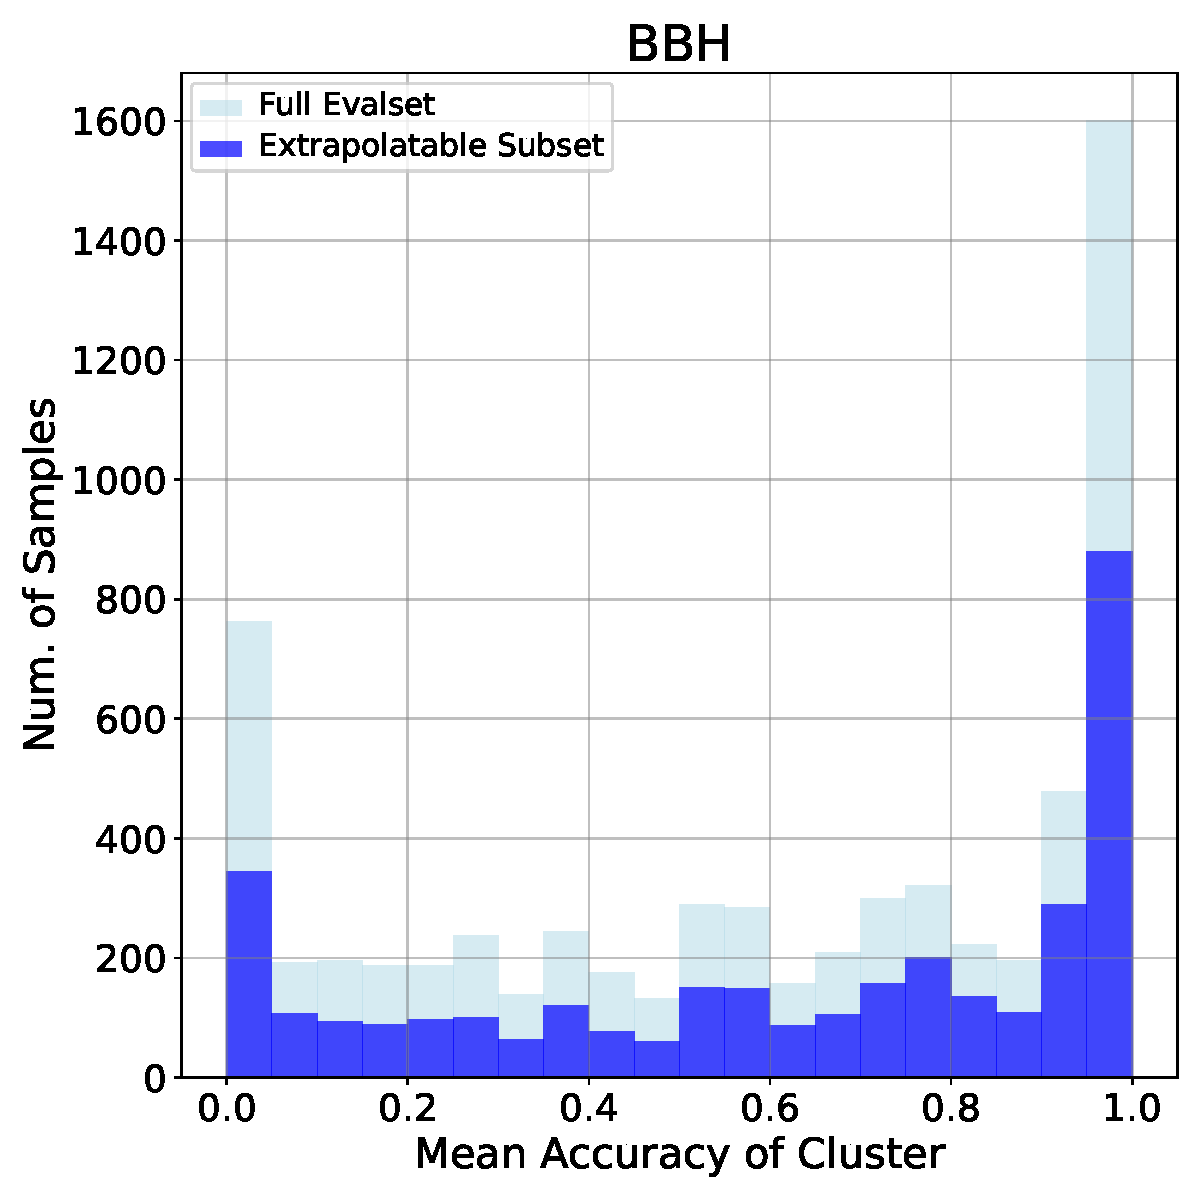
\includegraphics[width=\textwidth]{figures/appendix/difficulty_distributions/bbh.pdf}
        % \caption*{Title 1}
    \end{minipage}
    \begin{minipage}{0.24\textwidth}
        \centering
        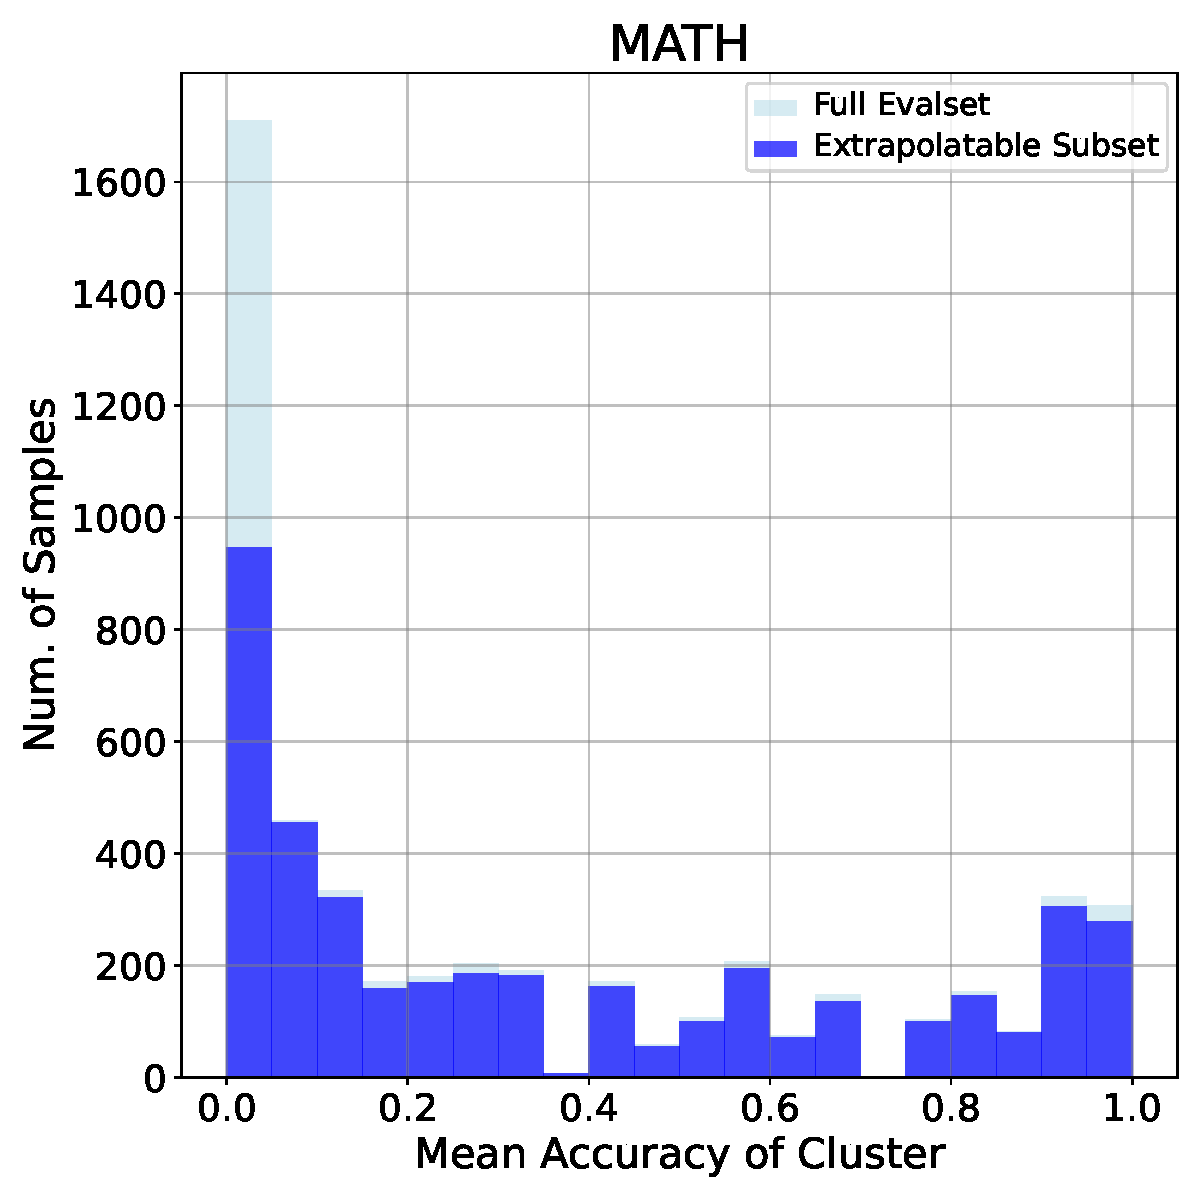
\includegraphics[width=\textwidth]{figures/appendix/difficulty_distributions/math.pdf}
        % \caption*{Title 2}
    \end{minipage}
    \begin{minipage}{0.24\textwidth}
        \centering
        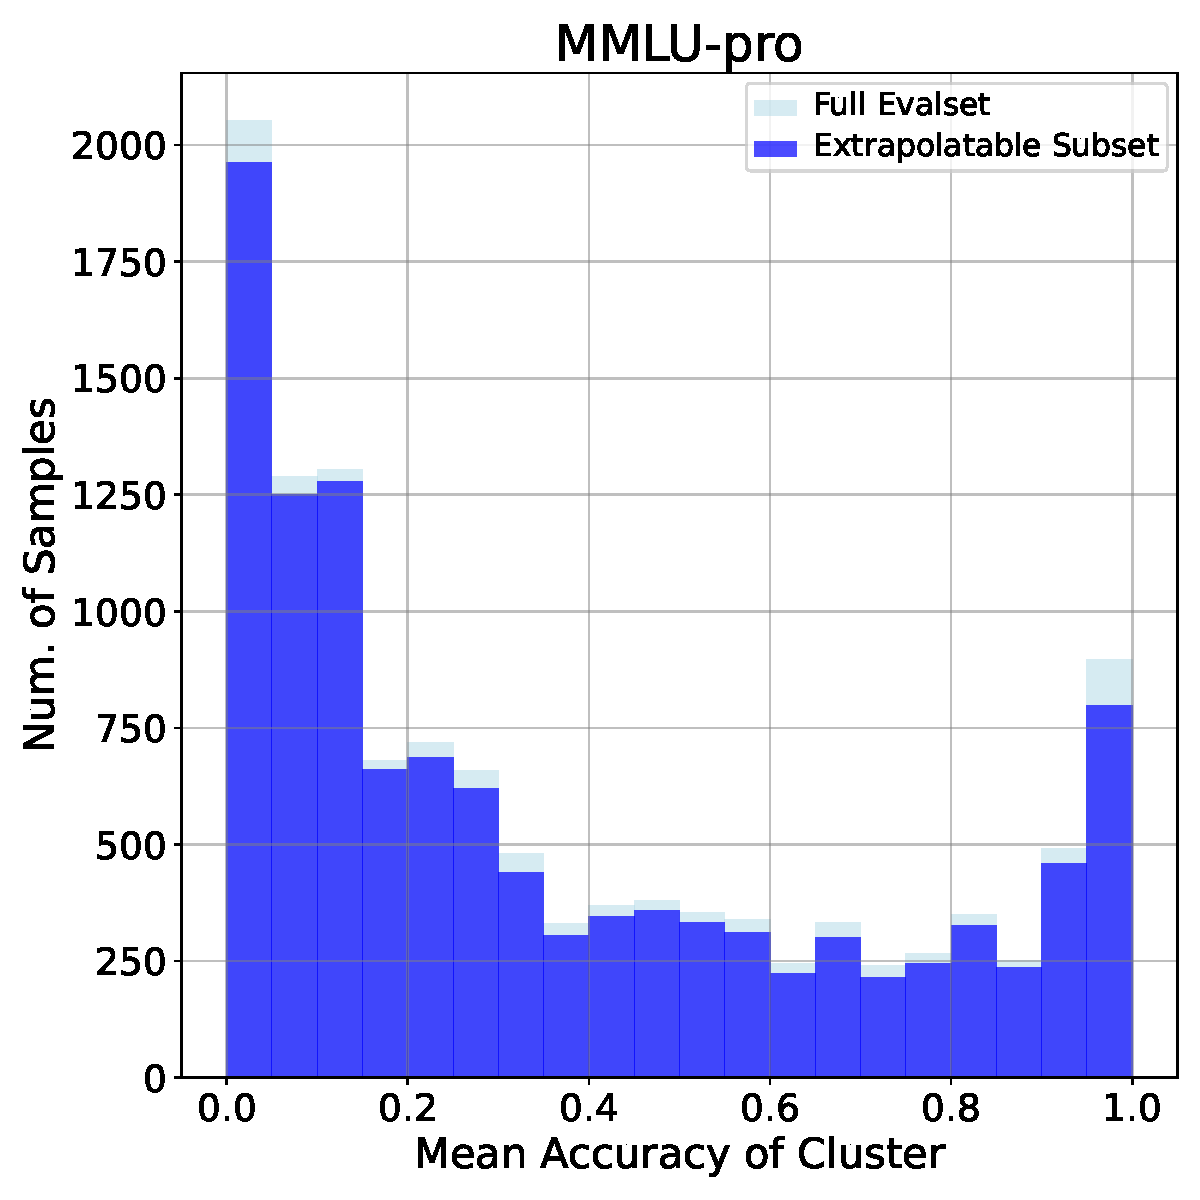
\includegraphics[width=\textwidth]{figures/appendix/difficulty_distributions/mmlu_pro.pdf}
        % \caption*{Title 3}
    \end{minipage}
    \begin{minipage}{0.24\textwidth}
        \centering
        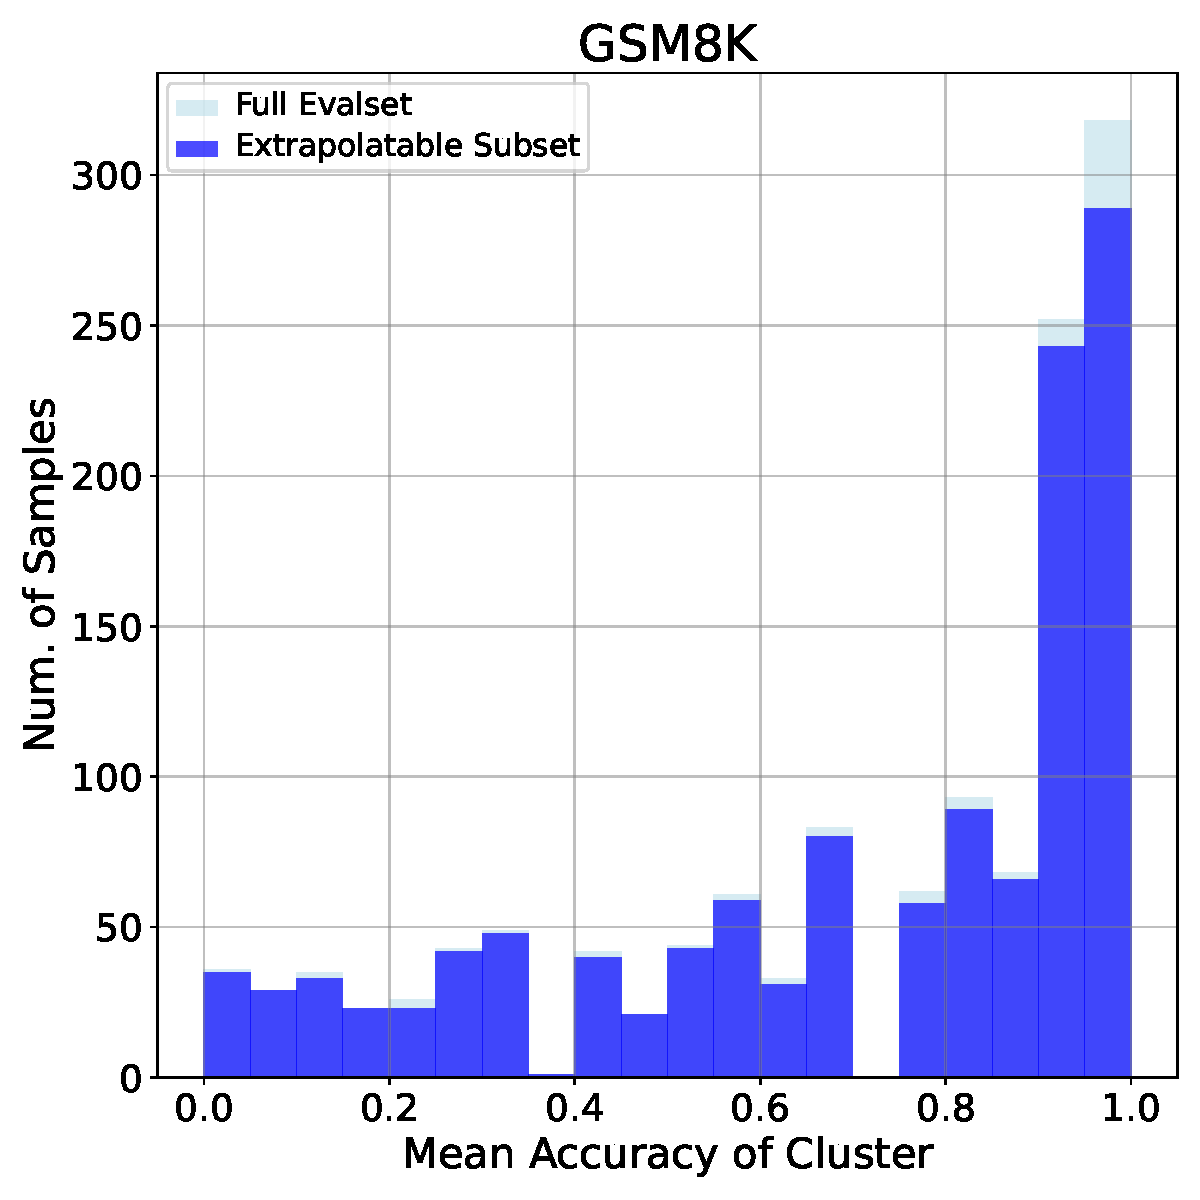
\includegraphics[width=\textwidth]{figures/appendix/difficulty_distributions/gsm8k.pdf}
        % \caption*{Title 4}
    \end{minipage}
    
    \vspace{0.5cm} % Add space between rows
    
    % Second row
    \begin{minipage}{0.24\textwidth}
        \centering
        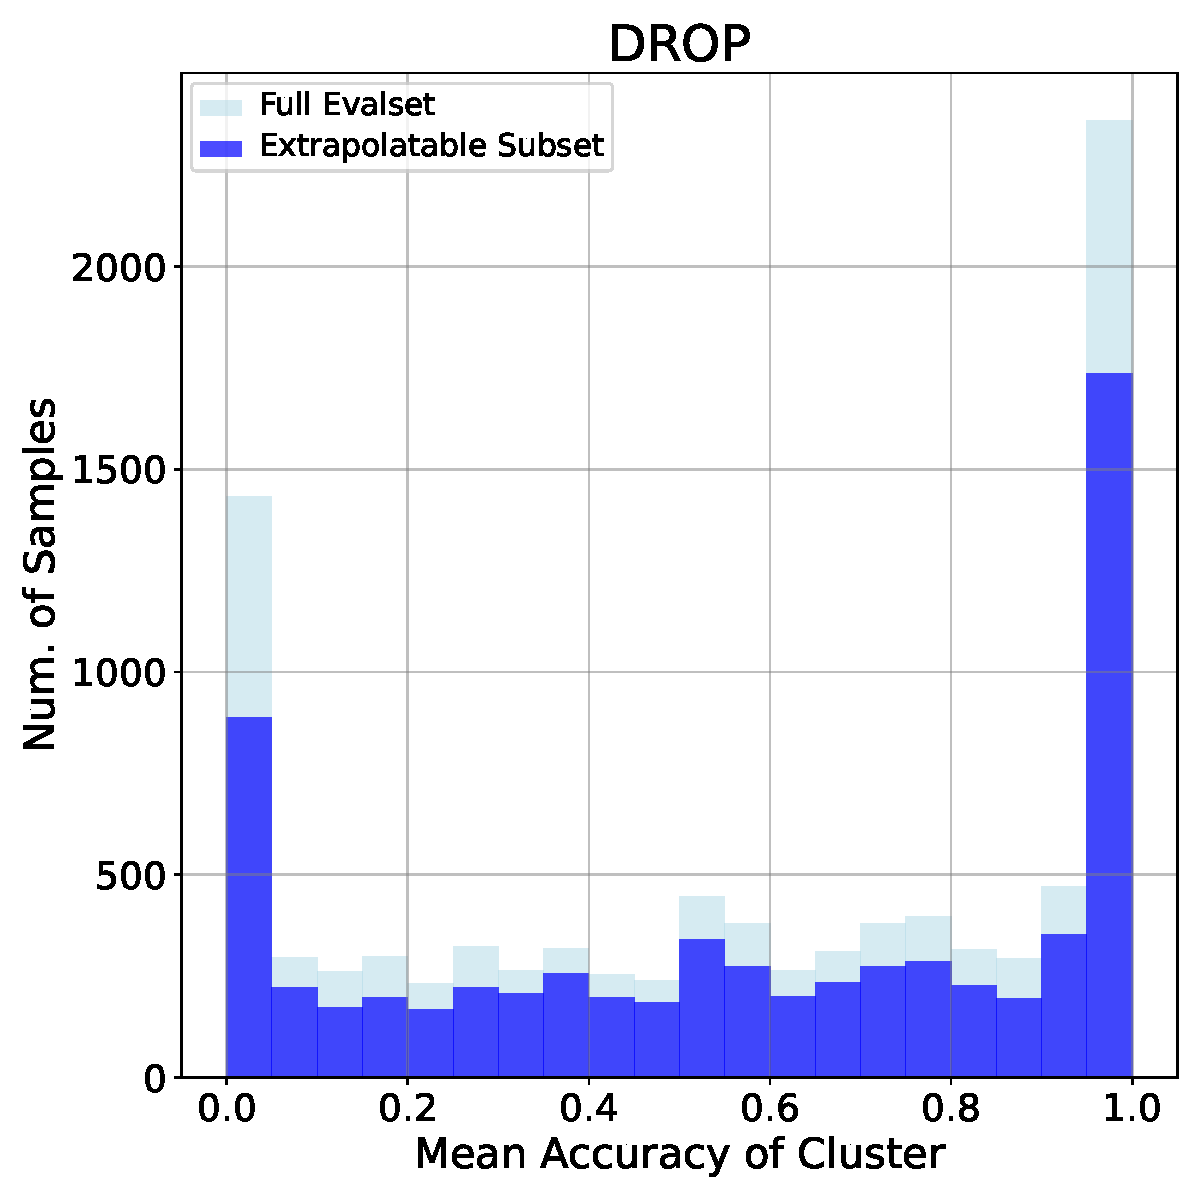
\includegraphics[width=\textwidth]{figures/appendix/difficulty_distributions/drop.pdf}
        % \caption*{Title 5}
    \end{minipage}
    \begin{minipage}{0.24\textwidth}
        \centering
        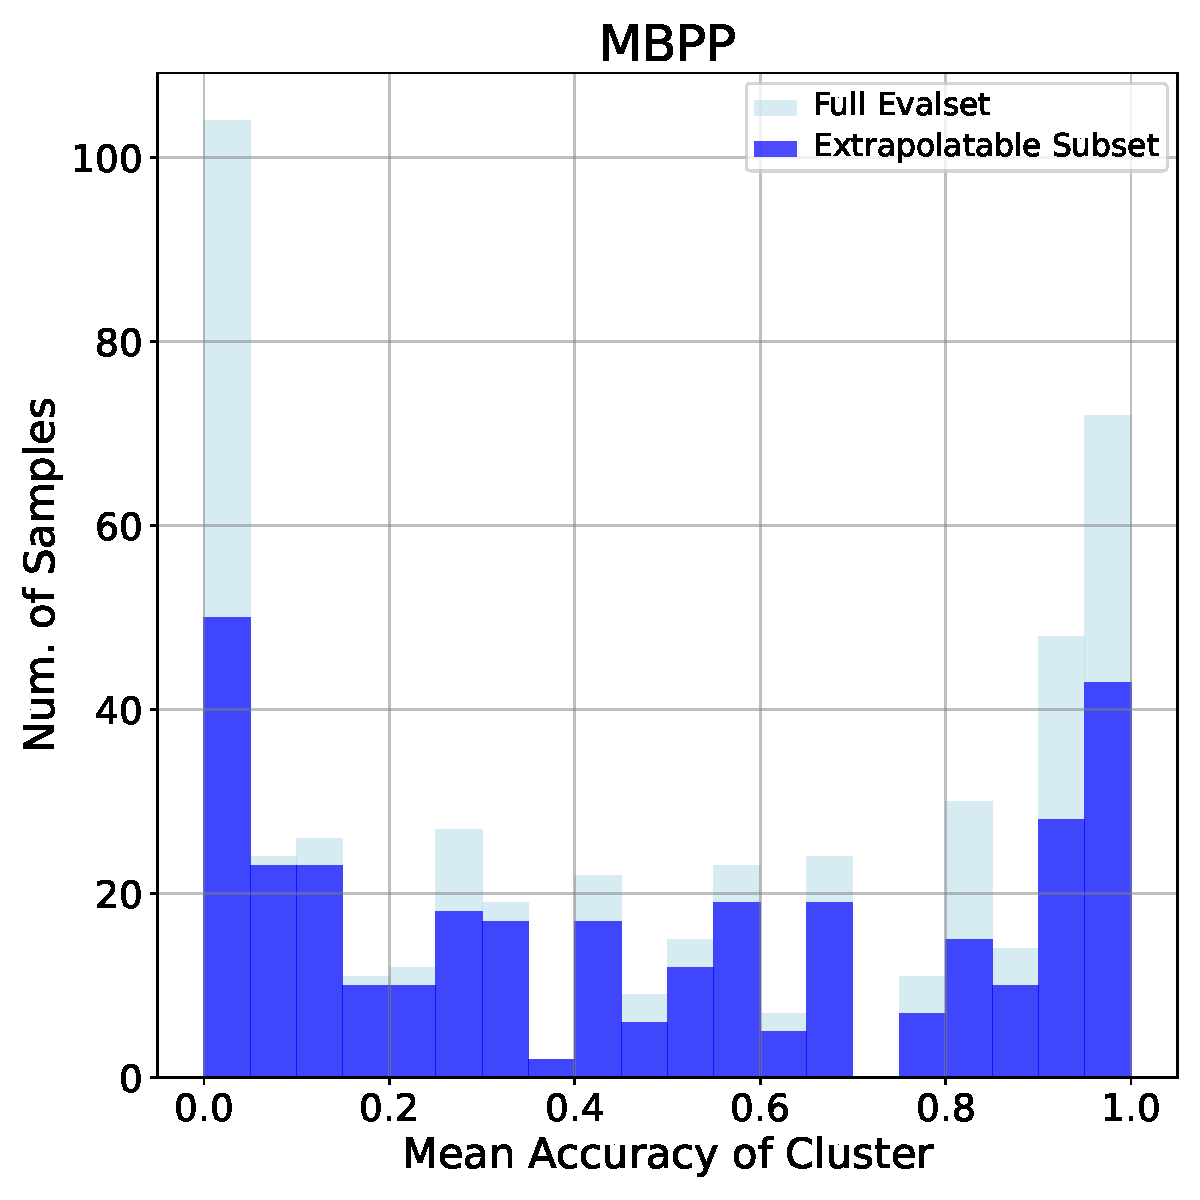
\includegraphics[width=\textwidth]{figures/appendix/difficulty_distributions/mbpp.pdf}
        % \caption*{Title 6}
    \end{minipage}
    \begin{minipage}{0.24\textwidth}
        \centering
        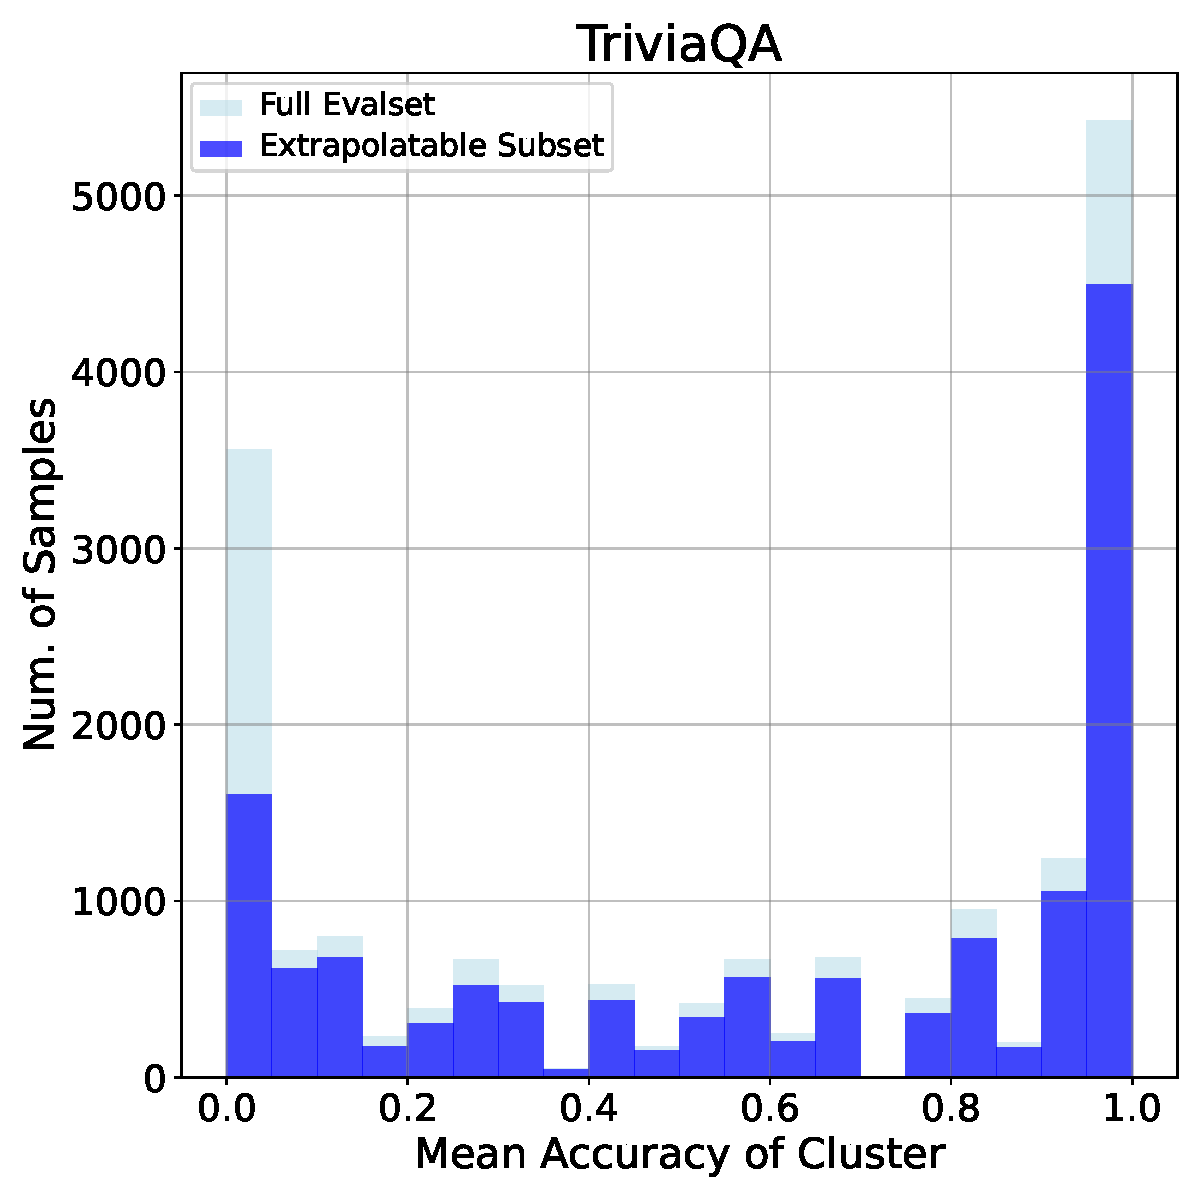
\includegraphics[width=\textwidth]{figures/appendix/difficulty_distributions/triviaqa.pdf}
        % \caption*{Title 7}
    \end{minipage}
    \begin{minipage}{0.24\textwidth}
        \centering
        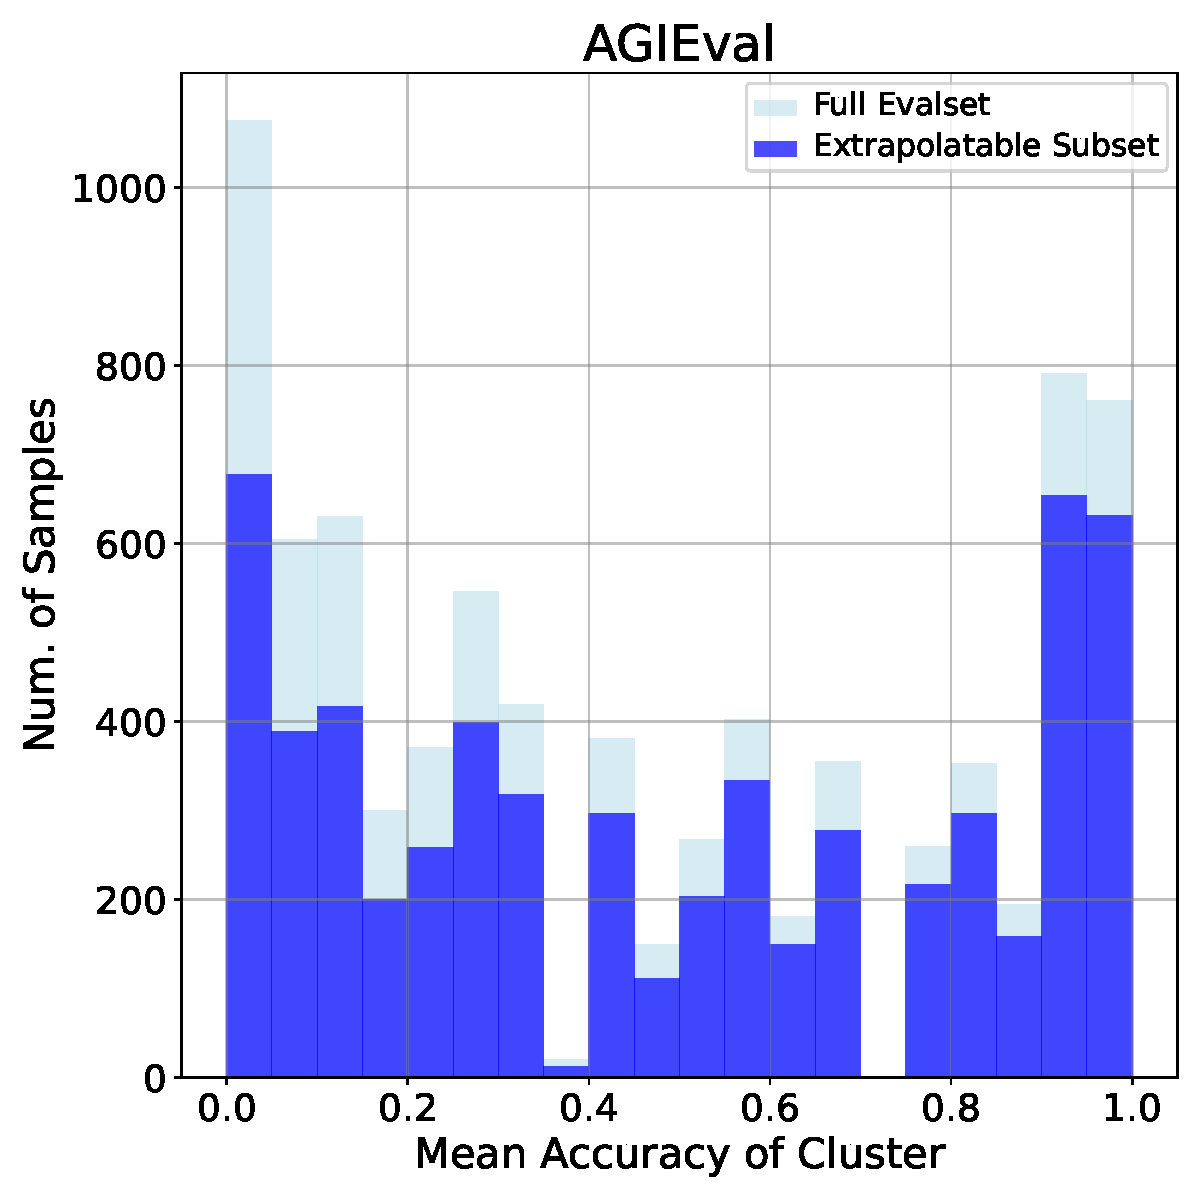
\includegraphics[width=\textwidth]{figures/appendix/difficulty_distributions/agieval.pdf}
        % \caption*{Title 8}
    \end{minipage}
    
    \caption{Difficulty distribution comparison on a 12B model between predictable subset and full evaluation set.}
    \label{fig:diff_dist}
\end{figure}


\renewcommand{\thefigure}{E\arabic{figure}}
\renewcommand{\thetable}{E\arabic{table}}
\renewcommand{\theproposition}{E.\arabic{proposition}}

\section{\anno{Computational Cost}}
\label{append:compute}
\anno{
The extra computational overhead of running COD is not expensive compared to training a series of small models with increasing parameter sizes. The main additional cost comes from performing 100 inference evaluations on the evaluation set for each small model (the cost of clustering algorithm is negligible compared to the inference cost). The computational complexity is $O(TMN)$, where $T$ is the number of evaluation runs, $M$ is the number of tokens for one evaluation, and $N$ is the maximum parameter size of the small models used for prediction. The corresponding token usage is $O(TM)$.

In particular, for an evaluation set requiring $1M$ tokens, a total of $100M$ tokens for small model inference is needed. In our experiments, the training token count for the 12B small model is $1.554T$. Considering that a training token is typically 3 times more costly than an inference token, the additional cost of COD is approximately $\frac{100M}{1.554T * 3} \approx 0.002\%$ of the training cost.
}

% \labubu{Furthermore, the cluster information for an evaluation set characterizes its difficulty distribution (including not only absolute difficulty but also the scaling features of the problems). This information is independent of the specific family of models being evaluated. Therefore, these clusters can be reused when estimating the capabilities of LLMs with new architectures, parameter counts, or training data.}

\section{Limitations}
\label{sec:limiations}

% \noindent\textbf{Influence of model structure.} Mixture-of-Experts (MoE) models excel in training and inference cost, and are widely used in production. In this work, we reveal the performance scaling on dense transformers, while prediction on MoE models is still underexplored.
% % 不过我们认为所提方法不会收到模型结构影响很多，如果我们把完整Pipeline应用在MoE模型上，我们同样预期能获得相似效果。
% However, we believe that the proposed method is not significantly affected by the model architecture. We expect similar results for MoE models.
% 我们只研究了恒定学习率的预训练能力预估，没有覆盖到退火阶段对指标的影响。该阶段通常采用更高质量的数据，可以快速提升模型能力，也因此Performance Prediction具有更大挑战。


\noindent\textbf{\camera{Compromised robustness due to excessive hyperparameter.}}
\camera{The complete pipeline of our proposed COD method incorporates several hyperparameters designed to constrain and refine the outcomes of various stages. These include the minimum intra-cluster sample size $K$, the adaptive bandwidth hyperparameter $Q$, and the maximum intra-cluster distance threshold $U$ for the clustering phase; parameters $a, b,$ and $c$ for filtering extrapolatable subsets during curve fitting; and the RMSE threshold $T$ utilized during the mapping process.

Regarding the clustering-related hyperparameters, they can be omitted if pre-computed cluster assignments are reused; otherwise, we provide empirically validated default values as reliable priors. For the remaining hyperparameters, we present comprehensive ablation studies in the paper, demonstrating that the final predictive performance is robust and relatively insensitive to these settings. Despite these mitigations, the reliance on a multi-parameter configuration may pose challenges to the COD method’s ease of deployment when generalizing to novel prediction scenarios.}
% 我们提出的COD方法的完整pipeline中存在较多的超参数用于约束各个阶段的效果，包括聚类时的最小类内样本数K、自适应带宽超参数Q、类内最大距离值，拟合曲线时用于筛选可外推子集的a、b、c，以及mapping时RMSE的阈值B。对于前三个聚类相关的超参数，如果复用已有聚类结果则可以省略；如果需要重新进行聚类，我们也提供了先验较为合理的参考值。对于后四个超参数，我们在文中给出了充足的超参消融实验验证了鲁棒性，证明最终预测效果对这些超参不敏感。尽管如此，较多的超参数还是使得COD方法在迁移到新预测场景下时的鲁棒性受到挑战。

\noindent\textbf{Category of evaluation sets.}
% 我们提出的Clustering-on-Difficulty Method对测试集题目数量有一点要求，过少的题目导致类簇指标不稳定从而无法有效预估。不过从测试集设计的角度看，一个具有良好预估性质的评估集可以更有效的通过小模型实验结果推广到大模型，对于模型迭代具有更好的指导意义。
%
%此外，针对Multi-choice类型题目，仅需要保证预测出正确选项概率大于其余选项，此时指标与模型真实的Passrate存在差异。考虑到更多的评估集采用Chain-of-Thoughts模式，我们没有覆盖近输出选项的选择题任务。
The proposed Clustering-on-Difficulty method requires a sufficient number of test cases, as too few samples can lead to unstable cluster metrics and ineffective estimation. From an evaluation set design perspective, an evaluation set with good predictive properties enables more effective generalization from small-scale to large-scale models, thus providing better guidance for model iteration.

\revise{Furthermore, we have not included multiple-choice tasks that require comparing the logits of correct options to calculate scores. These tasks creating a discrepancy between the answer loss and the model's true passrate, which violates the assumptions of the proposed Scaling Law for downstream task performance.}

\noindent\textbf{\camera{The prediction accuracy for smaller models is unsatisfactory.}}
\camera{Since our proposed COD (Clustering on Difficulty) method involves modeling the scaling of sample difficulty within the evaluation set, the clustering process requires a certain scale of models to participate in pass rate evaluation. This ensures an accurate estimation of sample difficulty. However, when predicting the performance of relatively smaller target models (e.g., around 10B parameters), the proxy models used for clustering and fitting are typically limited to even smaller scales (e.g., 2B). In such scenarios, a significant portion of samples may exhibit non-emergent or nascent emergent behaviors, making it challenging to accurately model difficulty features that scale with compute. Under these specific constraints, methods that perform sample-wise extrapolation—such as PassUntil~\citep{hu2023predicting}—tend to yield more robust predictive performance. Nonetheless, the primary utility of metric prediction lies in forecasting the downstream performance of significantly larger models. From this perspective, our COD method maintains broad applicability and significant value in mainstream scaling law research.}
% 由于我们提出的COD方法涉及对评估集样本难度scaling的建模，因此在聚类时需要一定规模的模型参与passrate评估，以保障对样本难度的准确估计。在预测smaller model（如10B左右）时，用于聚类、拟合的小模型最大可能也只有2B左右，此时会出现大量的未涌现或刚涌现的样本，无法准确建模随算力scaling的难度特征。在这种场景下，直接利用 passrate 指标 sample-wise外推再聚合的预测效果会更理想，如PassUntil方法。不过从另一个角度说，metric prediction方法更重要的应用还是预测更大的模型的下游指标，因此我们提出的COD方法依然有广泛的使用价值。

\noindent\textbf{Chain-of-thought performance prediction}.
% 我们提出的Scaling Law for Downstream Tasks~\cref{proof:task_scaling_law}假设了测试集评价模型直接给出答案的能力。但实际上越来越多的评测会允许模型进行思考后给出答案。Inference time scaling更进一步表明在数学、推理、代码等任务上，通过训练模型通过更长推理计算来完成任务可以大幅提升下游任务效果。
% 在推理过程或答案不唯一的情况下，模型在一个Task的Answer Loss与其Passrate不一定具有$p_\mathrm{ans}=\exp(-\mathrm{loss}_\mathrm{ans})$的关系。虽然我们的方案在该情况下保持其预估效果，但理论解释是不充分的。因此，我们把根据Chain-of-thought特性改进预估方法与扩充理论依据作为未来工作。
\cref{main:proof:task_scaling_law} assumes that evaluation sets directly assess models' ability to provide answers. However, increasingly more evaluations allow models to think before providing answers. Recent works on inference time scaling~\citep{snell2024scaling, bansal2024smaller} further demonstrate that for tasks involving mathematics, reasoning, and coding, training models to complete tasks through longer inference computation can significantly improve downstream task performance. In cases where the reasoning process or answers are not unique, the relationship between a model's answer loss and passrate on a task may not necessarily follow the exponential relationship between the answer loss and the sample passrate. \camera{Although our COD framework still achieves reasonable prediction performance in such scenarios, its theoretical foundation lacks sufficient explanation for the performance scaling of chain-of-thought based tasks.} Therefore, we consider improving prediction methods based on chain-of-thought characteristics and expanding theoretical foundations as future work.

% \noindent\textbf{\labubu{Complex Procedure.}}
% \labubu{Compared with current mainstream prediction methods (Loss-intermediate or End-to-end methods), the proposed COD requires more preparatory efforts and involves a more complex prediction process, which poses substantial challenges to both the reproduction of this method and its practical application in the prediction of LLMs. In future work, we will attempt to simplify the preparatory efforts and prediction process, or release a robust set of clustering labels for open-source evaluation datasets, thereby reducing the overhead for the academic community to reproduce or apply this method.}

% \section{Use of LLMs}
% \label{sec:llmuse}
% We utilized language models at the writing level, including checking for grammatical errors in the article, modifying expressions, and translating non-English information. The language models had no impact on the article's innovative contributions, experiments, or analytical perspectives.

\end{document}
